% Danger ... original file is in ../Curricula.in/Disciplines/Computing/tex/ this is ONLY a TEMP COPY !!!!!!!!!
\documentclass[a0]{a0poster}
\usepackage[utf8]{inputenc}

\input{current-institution}
\newcommand{\OutcomesVersion}[1]{}
\newcommand{\OutcomesList}[2]{}

\input{\InInstConfigDir/\currentinstitution}
\newcommand{\DocumentVersion}{2016}
\newcommand{\fecha}{\today}
\newcommand{\city}{Arequipa\xspace}
\newcommand{\country}{Peru\xspace}
\newcommand{\dictionary}{Español\xspace}
\newcommand{\SyllabusLangs}{Español,English}
\newcommand{\GraphVersion}{2\xspace}

\newcommand{\CurriculaVersion}{2016\xspace} % CS#-dependencies.tex: Malla 2006: 1, Malla 2010: 2, 
\newcommand{\YYYY}{2018\xspace}             % Plan 2006, 2018: Plan2018, 2021: Plan 2021
\newcommand{\Range}{1-10}                   % Plan 2010 1-8, Plan 2006 7-10   %   

           % Plan 2016 1-8, Plan 2006 7-10
\newcommand{\equivalences}{} %  {2006,2010}
\OutcomesVersion{V2}
\OutcomesList{V1}{a,b,c,d,e,f,g,h,i,j,k,l,m,n,o,p}
\OutcomesList{V2}{1,2,3,4,5,6,7}

\newcommand{\FacultadNameES}{Facultad de Ingeniería y Computación}
\newcommand{\FacultadNameEN}{School of Engineering and Computing}
\newcommand{\FacultadName}{}

\newcommand{\DepartmentNameES}{Ciencia de la Computación\xspace}
\newcommand{\DepartmentNameEN}{Department of Computer Science\xspace}
\newcommand{\DepartmentName}{\DepartmentNameES}

\newcommand{\SchoolShortNameES}{Ciencia de la Computación\xspace}
\newcommand{\SchoolShortNameEN}{Computer Science\xspace}
\newcommand{\SchoolShortName}{\SchoolShortNameES}

\newcommand{\SchoolFullNameES}{Escuela Profesional de Ciencia de la Computación\xspace}
\newcommand{\SchoolFullNameEN}{Undergraduate Program in Computer Science\xspace}
\newcommand{\SchoolFullName}{\SchoolFullNameES}

\newcommand{\SchoolFullNameBreakES}{Escuela Profesional de\\Ciencia de la Computación\xspace}
\newcommand{\SchoolFullNameBreakEN}{Undergraduate Program in\\Computer Science\xspace}
\newcommand{\SchoolFullNameBreak}{\SchoolFullNameBreakES}

\newcommand{\PosterTitle}{}

\newcommand{\SchoolAcro}{PPCS\xspace}
\newcommand{\SchoolURL}{\href{http://cs.ucsp.edu.pe}{http://cs.ucsp.edu.pe}\xspace}
\newcommand{\underlogotext}{}

\newcommand{\AcademicDegreeIssuedES}{Bachiller en Ciencia de la Computación\xspace}
\newcommand{\AcademicDegreeIssuedEN}{Bachelor in Computer Science\xspace}
\newcommand{\AcademicDegreeIssued}{\AcademicDegreeIssuedES}

\newcommand{\TitleIssuedES}{Licenciado en Ciencia de la Computación\xspace}
\newcommand{\TitleIssuedEN}{Professional in Computer Science\xspace}
\newcommand{\TitleIssued}{\TitleIssuedES}

\newcommand{\AcademicDegreeAndTitleES}%
{\begin{description}%
\item [Grado Académico: ] \AcademicDegreeIssued\xspace y% 
\item [Titulo Profesional: ] \TitleIssued%
\end{description}%
}

\newcommand{\AcademicDegreeAndTitleEN}%
{\begin{description}%
\item [Academic degree: ] \AcademicDegreeIssuedEN\xspace y% 
%\item [Titulo Profesional: ] \TitleIssued%
\end{description}%
}
\newcommand{\AcademicDegreeAndTitle}{\AcademicDegreeAndTitleES}

\newcommand{\doctitle}{Plan Curricular \YYYY\xspace del \SchoolFullName\\ \SchoolURL}

\newcommand{\AbstractIntro}{Este documento representa el informe final de la 
malla curricular \YYYY\xspace de la \SchoolFullName~de
la \University~(\textit{\InstitutionURL}) en la ciudad de \city-\country.}

\newcommand{\OtherKeyStones}%
{Un pilar que merece especial consideración en el caso de la \University~es el aspecto de 
valores humanos, básicos y cristianos debido a que forman parte fundamental 
de los lineamientos básicos de la existencia de la institución.\xspace}

\newcommand{\profileES}{%
El perfil profesional puede ser mejor entendido a partir de
\OnlyMainDoc{la Fig.~\ref{fig.cs} (Pág.~\pageref{fig.cs})}\OnlyPoster{las figuras del lado derecho}. 
Este profesional tiene como objetivo principal ser el impulsor del desarrollo de nuevas 
tecnologías computacionales con calidad internacional que puedan ser útiles a nivel local, nacional e internacional.
Nuestro perfil profesional también está orientado a ser generador de puestos de empleo a través de la innovación permanente. 
Nuestra formación profesional tiene 3 pilares fundamentales: 
un contenido computacional de acuerdo a normas internacionales (CS2013), una orientación marcada a la innovación ambos enriquecidos por una sólida
Formación Humana.
}
\newcommand{\profileEN}{%
The professional profile can be better understood from
\OnlyMainDoc{the Fig.~\ref{fig.cs} (Page~\pageref{fig.cs})}\OnlyPoster{the figures on the right side}.
This professional's main objective is to be the promoter of the development of new computational technologies with international quality that can be useful at a local, national and international level.
Our professional profile is also geared towards generating jobs through permanent innovation.
Our professional training has 3 fundamental pillars: a computational content according to international standards (CS2013), a marked orientation to innovation, 
both enriched by a solid Human Education.
}
\newcommand{\profile}{\profileES}

\newcommand{\missionES}{La Universidad Católica San Pablo es una comunidad académica animada por las orientaciones y vida de la Iglesia Católica que, 
a la luz de la fe y con el esfuerzo de la razón, busca la verdad y promueve la formación integral de la persona mediante actividades 
como la investigación, la enseñanza y la extensión, para contribuir con la 
configuración de la cultura conforme a la identidad y despliegue propios del ser humano.\xspace}

\newcommand{\missionEN}{Universidad Católica San Pablo is an academic community animated by the orientations and life of the Catholic Church that, 
in the light of faith and with the effort of reason, 
seeks the truth and promotes the integral formation of the person through activities 
such as research, teaching and extension, to contribute to the 
configuration of culture according to the identity and deployment of the human being.\xspace}
\newcommand{\mission}{\missionES}

\newcommand{\visionEN}{\missionEN}
\newcommand{\visionES}{\missionES}
\newcommand{\vision}{\visionES}

\newcommand{\HTMLFootnote}{{Generado por <A HREF='http://socios.spc.org.pe/ecuadros/'>Ernesto Cuadros-Vargas</A> <ecuadros AT spc.org.pe>, 
                           <A HREF='http://www.spc.org.pe/'>Sociedad Peruana de Computaci&oacute;n-Peru</A>, 
                           basado en el modelo de la Computing Curricula de 
                           <A HREF='http://www.computer.org/'>IEEE-CS</A>/<A HREF='http://www.acm.org/'>ACM</A>}}

\newcommand{\Copyrights}{Generado por Ernesto Cuadros-Vargas (ecuadros AT spc.org.pe), 
                           Sociedad Peruana de Computación (http://www.spc.org.pe/), 
                           %Universidad de Ingenier\'{i}a y Tecnolog\'{i}a (UTEC) (http://www.utec.edu.pe) \country 
                           basado en la {\it Computing Curricula} de 
                           IEEE-CS (http://www.computer.org) y ACM (http://www.acm.org/)}

\usepackage{array}
\usepackage{a0poster}
\usepackage{pst-blur}
\usepackage{paralist}
\usepackage{\InStyAllDir/parallel}
\usepackage[top=0cm,bottom=0cm,left=1cm,right=1cm]{geometry}
\usepackage{lmodern}
\usepackage[T1]{fontenc}

%%%%%%%%%%%%%%%%%%%%%%%%%%%%%%%%%%%%%%%%%%%%%%%%%%%%%%%%%%%%%%
\usepackage[printonlyused]{acronym}
\usepackage[spanish]{babel}
\usepackage[dvips]{hyperref}
\usepackage{amsmath}
\usepackage{amssymb}
\usepackage{graphics}
\usepackage{graphicx}
%\usepackage{./in/sty/hlundef} %If error just comment it, it is to highlight unreferenced citations (?)
\usepackage{ae}
\usepackage{tabularx}
\usepackage{xspace}
\usepackage{pstricks}
\usepackage{pst-tree}
\usepackage{pst-node}
\usepackage{xspace}
\usepackage{lscape}
\usepackage{html}
\hypersetup{  
    pdfauthor = {Ernesto Cuadros-Vargas (ecuadros@spc.org.pe)},
    pdfproducer = {Ernesto Cuadros-Vargas (ecuadros@spc.org.pe)},
    pdfpagemode=FullScreen,
    pdfsubject = {Computing Curricula},
    pdftitle = {Plan Curricular \YYYY},
    pdfkeywords = {Computing Curricula, Peruvian Computing Society, Sociedad Peruana de Computación},
    bookmarksopen=true,
    breaklinks=true,
    raiselinks=true,
}  


\usepackage{multirow}
\usepackage{multicol}
\usepackage{rotating}
%\usepackage{titlesec}
\usepackage{xkeyval}
% \usepackage{color}
\usepackage{colortbl}
\usepackage[most]{tcolorbox}

%%%%%%%%%%%%%%%%%%%%%%%%%%%%%%%%%%%%%%%%%%%%%%%%%%%%%%%%%%%%%%
% \newcommand{\logoheight}{<LOGO_WIDTH>}
\newcommand{\titlesize}{0.70\textwidth}
\newcommand{\posterbackground}{<POSTER_RIGHT_BG>}

%\newcommand{\posterbackground}{0.25,0.41,0.88}
\newcommand{\captionsize}{\footnotesize}
\newcommand{\OnlyMainDoc}[1]{}
\newcommand{\OnlyPoster}[1]{#1\xspace}  
\newcommand{\Cblur}[1]{\psblurbox[framesep=5pt,shadow=false,blur=true,shadowsize=6pt,blurradius=3pt,blursteps=60,framearc=0.05,linecolor=black]{#1} }
\usepackage{poster-macros}
\usepackage{\InStyDir/bok-macros}
\newrgbcolor{antiquewhite}{0.980392156862745 0.92156862745098 0.843137254901961}
\newrgbcolor{antiquewhite1}{1 0.937254901960784 0.858823529411765}
\newrgbcolor{antiquewhite2}{0.933333333333333 0.874509803921569 0.8}
\newrgbcolor{antiquewhite3}{0.803921568627451 0.752941176470588 0.690196078431373}
\newrgbcolor{antiquewhite4}{0.545098039215686 0.513725490196078 0.470588235294118}
\newrgbcolor{aquamarine}{0.498039215686275 1 0.831372549019608}
\newrgbcolor{aquamarine1}{0.498039215686275 1 0.831372549019608}
\newrgbcolor{aquamarine2}{0.462745098039216 0.933333333333333 0.776470588235294}
\newrgbcolor{aquamarine3}{0.4 0.803921568627451 0.666666666666667}
\newrgbcolor{aquamarine4}{0.270588235294118 0.545098039215686 0.454901960784314}
\newrgbcolor{azure}{0.941176470588235 1 1}
\newrgbcolor{azure1}{0.941176470588235 1 1}
\newrgbcolor{azure2}{0.87843137254902 0.933333333333333 0.933333333333333}
\newrgbcolor{azure3}{0.756862745098039 0.803921568627451 0.803921568627451}
\newrgbcolor{azure4}{0.513725490196078 0.545098039215686 0.545098039215686}
\newrgbcolor{beige}{0.96078431372549 0.96078431372549 0.862745098039216}
\newrgbcolor{bisque}{1 0.894117647058824 0.768627450980392}
\newrgbcolor{bisque1}{1 0.894117647058824 0.768627450980392}
\newrgbcolor{bisque2}{0.933333333333333 0.835294117647059 0.717647058823529}
\newrgbcolor{bisque3}{0.803921568627451 0.717647058823529 0.619607843137255}
\newrgbcolor{bisque4}{0.545098039215686 0.490196078431373 0.419607843137255}
\newrgbcolor{black}{0 0 0}
\newrgbcolor{blanchedalmond}{1 0.92156862745098 0.803921568627451}
\newrgbcolor{blue}{0 0 1}
\newrgbcolor{blue1}{0 0 1}
\newrgbcolor{blue2}{0 0 0.933333333333333}
\newrgbcolor{blue3}{0 0 0.803921568627451}
\newrgbcolor{blue4}{0 0 0.545098039215686}
\newrgbcolor{blueviolet}{0.541176470588235 0.168627450980392 0.886274509803922}
\newrgbcolor{brown}{0.647058823529412 0.164705882352941 0.164705882352941}
\newrgbcolor{brown1}{1 0.250980392156863 0.250980392156863}
\newrgbcolor{brown2}{0.933333333333333 0.231372549019608 0.231372549019608}
\newrgbcolor{brown3}{0.803921568627451 0.2 0.2}
\newrgbcolor{brown4}{0.545098039215686 0.137254901960784 0.137254901960784}
\newrgbcolor{burlywood}{0.870588235294118 0.72156862745098 0.529411764705882}
\newrgbcolor{burlywood1}{1 0.827450980392157 0.607843137254902}
\newrgbcolor{burlywood2}{0.933333333333333 0.772549019607843 0.568627450980392}
\newrgbcolor{burlywood3}{0.803921568627451 0.666666666666667 0.490196078431373}
\newrgbcolor{burlywood4}{0.545098039215686 0.450980392156863 0.333333333333333}
\newrgbcolor{cadetblue}{0.372549019607843 0.619607843137255 0.627450980392157}
\newrgbcolor{cadetblue1}{0.596078431372549 0.96078431372549 1}
\newrgbcolor{cadetblue2}{0.556862745098039 0.898039215686275 0.933333333333333}
\newrgbcolor{cadetblue3}{0.47843137254902 0.772549019607843 0.803921568627451}
\newrgbcolor{cadetblue4}{0.325490196078431 0.525490196078431 0.545098039215686}
\newrgbcolor{chartreuse}{0.498039215686275 1 0}
\newrgbcolor{chartreuse1}{0.498039215686275 1 0}
\newrgbcolor{chartreuse2}{0.462745098039216 0.933333333333333 0}
\newrgbcolor{chartreuse3}{0.4 0.803921568627451 0}
\newrgbcolor{chartreuse4}{0.270588235294118 0.545098039215686 0}
\newrgbcolor{chocolate}{0.823529411764706 0.411764705882353 0.117647058823529}
\newrgbcolor{chocolate1}{1 0.498039215686275 0.141176470588235}
\newrgbcolor{chocolate2}{0.933333333333333 0.462745098039216 0.129411764705882}
\newrgbcolor{chocolate3}{0.803921568627451 0.4 0.113725490196078}
\newrgbcolor{chocolate4}{0.545098039215686 0.270588235294118 0.0745098039215686}
\newrgbcolor{coral}{1 0.498039215686275 0.313725490196078}
\newrgbcolor{coral1}{1 0.447058823529412 0.337254901960784}
\newrgbcolor{coral2}{0.933333333333333 0.415686274509804 0.313725490196078}
\newrgbcolor{coral3}{0.803921568627451 0.356862745098039 0.270588235294118}
\newrgbcolor{coral4}{0.545098039215686 0.243137254901961 0.184313725490196}
\newrgbcolor{cornflowerblue}{0.392156862745098 0.584313725490196 0.929411764705882}
\newrgbcolor{cornsilk}{1 0.972549019607843 0.862745098039216}
\newrgbcolor{cornsilk1}{1 0.972549019607843 0.862745098039216}
\newrgbcolor{cornsilk2}{0.933333333333333 0.909803921568627 0.803921568627451}
\newrgbcolor{cornsilk3}{0.803921568627451 0.784313725490196 0.694117647058824}
\newrgbcolor{cornsilk4}{0.545098039215686 0.533333333333333 0.470588235294118}
\newrgbcolor{crimson}{0.862745098039216 0.0784313725490196 0.235294117647059}
\newrgbcolor{cyan}{0 1 1}
\newrgbcolor{cyan1}{0 1 1}
\newrgbcolor{cyan2}{0 0.933333333333333 0.933333333333333}
\newrgbcolor{cyan3}{0 0.803921568627451 0.803921568627451}
\newrgbcolor{cyan4}{0 0.545098039215686 0.545098039215686}
\newrgbcolor{darkgoldenrod}{0.72156862745098 0.525490196078431 0.0431372549019608}
\newrgbcolor{darkgoldenrod1}{1 0.725490196078431 0.0588235294117647}
\newrgbcolor{darkgoldenrod2}{0.933333333333333 0.67843137254902 0.0549019607843137}
\newrgbcolor{darkgoldenrod3}{0.803921568627451 0.584313725490196 0.0470588235294118}
\newrgbcolor{darkgoldenrod4}{0.545098039215686 0.396078431372549 0.0313725490196078}
\newrgbcolor{darkgreen}{0 0.392156862745098 0}
\newrgbcolor{darkkhaki}{0.741176470588235 0.717647058823529 0.419607843137255}
\newrgbcolor{darkolivegreen}{0.333333333333333 0.419607843137255 0.184313725490196}
\newrgbcolor{darkolivegreen1}{0.792156862745098 1 0.43921568627451}
\newrgbcolor{darkolivegreen2}{0.737254901960784 0.933333333333333 0.407843137254902}
\newrgbcolor{darkolivegreen3}{0.635294117647059 0.803921568627451 0.352941176470588}
\newrgbcolor{darkolivegreen4}{0.431372549019608 0.545098039215686 0.23921568627451}
\newrgbcolor{darkorange}{1 0.549019607843137 0}
\newrgbcolor{darkorange1}{1 0.498039215686275 0}
\newrgbcolor{darkorange2}{0.933333333333333 0.462745098039216 0}
\newrgbcolor{darkorange3}{0.803921568627451 0.4 0}
\newrgbcolor{darkorange4}{0.545098039215686 0.270588235294118 0}
\newrgbcolor{darkorchid}{0.6 0.196078431372549 0.8}
\newrgbcolor{darkorchid1}{0.749019607843137 0.243137254901961 1}
\newrgbcolor{darkorchid2}{0.698039215686274 0.227450980392157 0.933333333333333}
\newrgbcolor{darkorchid3}{0.603921568627451 0.196078431372549 0.803921568627451}
\newrgbcolor{darkorchid4}{0.407843137254902 0.133333333333333 0.545098039215686}
\newrgbcolor{darksalmon}{0.913725490196078 0.588235294117647 0.47843137254902}
\newrgbcolor{darkseagreen}{0.56078431372549 0.737254901960784 0.56078431372549}
\newrgbcolor{darkseagreen1}{0.756862745098039 1 0.756862745098039}
\newrgbcolor{darkseagreen2}{0.705882352941177 0.933333333333333 0.705882352941177}
\newrgbcolor{darkseagreen3}{0.607843137254902 0.803921568627451 0.607843137254902}
\newrgbcolor{darkseagreen4}{0.411764705882353 0.545098039215686 0.411764705882353}
\newrgbcolor{darkslateblue}{0.282352941176471 0.23921568627451 0.545098039215686}
\newrgbcolor{darkslategray}{0.184313725490196 0.309803921568627 0.309803921568627}
\newrgbcolor{darkslategray1}{0.592156862745098 1 1}
\newrgbcolor{darkslategray2}{0.552941176470588 0.933333333333333 0.933333333333333}
\newrgbcolor{darkslategray3}{0.474509803921569 0.803921568627451 0.803921568627451}
\newrgbcolor{darkslategray4}{0.32156862745098 0.545098039215686 0.545098039215686}
\newrgbcolor{darkslategrey}{0.184313725490196 0.309803921568627 0.309803921568627}
\newrgbcolor{darkturquoise}{0 0.807843137254902 0.819607843137255}
\newrgbcolor{darkviolet}{0.580392156862745 0 0.827450980392157}
\newrgbcolor{deeppink}{1 0.0784313725490196 0.576470588235294}
\newrgbcolor{deeppink1}{1 0.0784313725490196 0.576470588235294}
\newrgbcolor{deeppink2}{0.933333333333333 0.0705882352941176 0.537254901960784}
\newrgbcolor{deeppink3}{0.803921568627451 0.0627450980392157 0.462745098039216}
\newrgbcolor{deeppink4}{0.545098039215686 0.0392156862745098 0.313725490196078}
\newrgbcolor{deepskyblue}{0 0.749019607843137 1}
\newrgbcolor{deepskyblue1}{0 0.749019607843137 1}
\newrgbcolor{deepskyblue2}{0 0.698039215686274 0.933333333333333}
\newrgbcolor{deepskyblue3}{0 0.603921568627451 0.803921568627451}
\newrgbcolor{deepskyblue4}{0 0.407843137254902 0.545098039215686}
\newrgbcolor{dimgray}{0.411764705882353 0.411764705882353 0.411764705882353}
\newrgbcolor{dimgrey}{0.411764705882353 0.411764705882353 0.411764705882353}
\newrgbcolor{dodgerblue}{0.117647058823529 0.564705882352941 1}
\newrgbcolor{dodgerblue1}{0.117647058823529 0.564705882352941 1}
\newrgbcolor{dodgerblue2}{0.109803921568627 0.525490196078431 0.933333333333333}
\newrgbcolor{dodgerblue3}{0.0941176470588235 0.454901960784314 0.803921568627451}
\newrgbcolor{dodgerblue4}{0.0627450980392157 0.305882352941176 0.545098039215686}
\newrgbcolor{firebrick}{0.698039215686274 0.133333333333333 0.133333333333333}
\newrgbcolor{firebrick1}{1 0.188235294117647 0.188235294117647}
\newrgbcolor{firebrick2}{0.933333333333333 0.172549019607843 0.172549019607843}
\newrgbcolor{firebrick3}{0.803921568627451 0.149019607843137 0.149019607843137}
\newrgbcolor{firebrick4}{0.545098039215686 0.101960784313725 0.101960784313725}
\newrgbcolor{floralwhite}{1 0.980392156862745 0.941176470588235}
\newrgbcolor{forestgreen}{0.133333333333333 0.545098039215686 0.133333333333333}
\newrgbcolor{gainsboro}{0.862745098039216 0.862745098039216 0.862745098039216}
\newrgbcolor{ghostwhite}{0.972549019607843 0.972549019607843 1}
\newrgbcolor{gold}{1 0.843137254901961 0}
\newrgbcolor{gold1}{1 0.843137254901961 0}
\newrgbcolor{gold2}{0.933333333333333 0.788235294117647 0}
\newrgbcolor{gold3}{0.803921568627451 0.67843137254902 0}
\newrgbcolor{gold4}{0.545098039215686 0.458823529411765 0}
\newrgbcolor{goldenrod}{0.854901960784314 0.647058823529412 0.125490196078431}
\newrgbcolor{goldenrod1}{1 0.756862745098039 0.145098039215686}
\newrgbcolor{goldenrod2}{0.933333333333333 0.705882352941177 0.133333333333333}
\newrgbcolor{goldenrod3}{0.803921568627451 0.607843137254902 0.113725490196078}
\newrgbcolor{goldenrod4}{0.545098039215686 0.411764705882353 0.0784313725490196}
\newrgbcolor{gray}{0.752941176470588 0.752941176470588 0.752941176470588}
\newrgbcolor{gray0}{0 0 0}
\newrgbcolor{gray1}{0.0117647058823529 0.0117647058823529 0.0117647058823529}
\newrgbcolor{gray2}{0.0196078431372549 0.0196078431372549 0.0196078431372549}
\newrgbcolor{gray3}{0.0313725490196078 0.0313725490196078 0.0313725490196078}
\newrgbcolor{gray4}{0.0392156862745098 0.0392156862745098 0.0392156862745098}
\newrgbcolor{gray5}{0.0509803921568627 0.0509803921568627 0.0509803921568627}
\newrgbcolor{gray6}{0.0588235294117647 0.0588235294117647 0.0588235294117647}
\newrgbcolor{gray7}{0.0705882352941176 0.0705882352941176 0.0705882352941176}
\newrgbcolor{gray8}{0.0784313725490196 0.0784313725490196 0.0784313725490196}
\newrgbcolor{gray9}{0.0901960784313725 0.0901960784313725 0.0901960784313725}
\newrgbcolor{gray10}{0.101960784313725 0.101960784313725 0.101960784313725}
\newrgbcolor{gray11}{0.109803921568627 0.109803921568627 0.109803921568627}
\newrgbcolor{gray12}{0.12156862745098 0.12156862745098 0.12156862745098}
\newrgbcolor{gray13}{0.129411764705882 0.129411764705882 0.129411764705882}
\newrgbcolor{gray14}{0.141176470588235 0.141176470588235 0.141176470588235}
\newrgbcolor{gray15}{0.149019607843137 0.149019607843137 0.149019607843137}
\newrgbcolor{gray16}{0.16078431372549 0.16078431372549 0.16078431372549}
\newrgbcolor{gray17}{0.168627450980392 0.168627450980392 0.168627450980392}
\newrgbcolor{gray18}{0.180392156862745 0.180392156862745 0.180392156862745}
\newrgbcolor{gray19}{0.188235294117647 0.188235294117647 0.188235294117647}
\newrgbcolor{gray20}{0.2 0.2 0.2}
\newrgbcolor{gray21}{0.211764705882353 0.211764705882353 0.211764705882353}
\newrgbcolor{gray22}{0.219607843137255 0.219607843137255 0.219607843137255}
\newrgbcolor{gray23}{0.231372549019608 0.231372549019608 0.231372549019608}
\newrgbcolor{gray24}{0.23921568627451 0.23921568627451 0.23921568627451}
\newrgbcolor{gray25}{0.250980392156863 0.250980392156863 0.250980392156863}
\newrgbcolor{gray26}{0.258823529411765 0.258823529411765 0.258823529411765}
\newrgbcolor{gray27}{0.270588235294118 0.270588235294118 0.270588235294118}
\newrgbcolor{gray28}{0.27843137254902 0.27843137254902 0.27843137254902}
\newrgbcolor{gray29}{0.290196078431373 0.290196078431373 0.290196078431373}
\newrgbcolor{gray30}{0.301960784313725 0.301960784313725 0.301960784313725}
\newrgbcolor{gray31}{0.309803921568627 0.309803921568627 0.309803921568627}
\newrgbcolor{gray32}{0.32156862745098 0.32156862745098 0.32156862745098}
\newrgbcolor{gray33}{0.329411764705882 0.329411764705882 0.329411764705882}
\newrgbcolor{gray34}{0.341176470588235 0.341176470588235 0.341176470588235}
\newrgbcolor{gray35}{0.349019607843137 0.349019607843137 0.349019607843137}
\newrgbcolor{gray36}{0.36078431372549 0.36078431372549 0.36078431372549}
\newrgbcolor{gray37}{0.368627450980392 0.368627450980392 0.368627450980392}
\newrgbcolor{gray38}{0.380392156862745 0.380392156862745 0.380392156862745}
\newrgbcolor{gray39}{0.388235294117647 0.388235294117647 0.388235294117647}
\newrgbcolor{gray40}{0.4 0.4 0.4}
\newrgbcolor{gray41}{0.411764705882353 0.411764705882353 0.411764705882353}
\newrgbcolor{gray42}{0.419607843137255 0.419607843137255 0.419607843137255}
\newrgbcolor{gray43}{0.431372549019608 0.431372549019608 0.431372549019608}
\newrgbcolor{gray44}{0.43921568627451 0.43921568627451 0.43921568627451}
\newrgbcolor{gray45}{0.450980392156863 0.450980392156863 0.450980392156863}
\newrgbcolor{gray46}{0.458823529411765 0.458823529411765 0.458823529411765}
\newrgbcolor{gray47}{0.470588235294118 0.470588235294118 0.470588235294118}
\newrgbcolor{gray48}{0.47843137254902 0.47843137254902 0.47843137254902}
\newrgbcolor{gray49}{0.490196078431373 0.490196078431373 0.490196078431373}
\newrgbcolor{gray50}{0.498039215686275 0.498039215686275 0.498039215686275}
\newrgbcolor{gray51}{0.509803921568627 0.509803921568627 0.509803921568627}
\newrgbcolor{gray52}{0.52156862745098 0.52156862745098 0.52156862745098}
\newrgbcolor{gray53}{0.529411764705882 0.529411764705882 0.529411764705882}
\newrgbcolor{gray54}{0.541176470588235 0.541176470588235 0.541176470588235}
\newrgbcolor{gray55}{0.549019607843137 0.549019607843137 0.549019607843137}
\newrgbcolor{gray56}{0.56078431372549 0.56078431372549 0.56078431372549}
\newrgbcolor{gray57}{0.568627450980392 0.568627450980392 0.568627450980392}
\newrgbcolor{gray58}{0.580392156862745 0.580392156862745 0.580392156862745}
\newrgbcolor{gray59}{0.588235294117647 0.588235294117647 0.588235294117647}
\newrgbcolor{gray60}{0.6 0.6 0.6}
\newrgbcolor{gray61}{0.611764705882353 0.611764705882353 0.611764705882353}
\newrgbcolor{gray62}{0.619607843137255 0.619607843137255 0.619607843137255}
\newrgbcolor{gray63}{0.631372549019608 0.631372549019608 0.631372549019608}
\newrgbcolor{gray64}{0.63921568627451 0.63921568627451 0.63921568627451}
\newrgbcolor{gray65}{0.650980392156863 0.650980392156863 0.650980392156863}
\newrgbcolor{gray66}{0.658823529411765 0.658823529411765 0.658823529411765}
\newrgbcolor{gray67}{0.670588235294118 0.670588235294118 0.670588235294118}
\newrgbcolor{gray68}{0.67843137254902 0.67843137254902 0.67843137254902}
\newrgbcolor{gray69}{0.690196078431373 0.690196078431373 0.690196078431373}
\newrgbcolor{gray70}{0.701960784313725 0.701960784313725 0.701960784313725}
\newrgbcolor{gray71}{0.709803921568627 0.709803921568627 0.709803921568627}
\newrgbcolor{gray72}{0.72156862745098 0.72156862745098 0.72156862745098}
\newrgbcolor{gray73}{0.729411764705882 0.729411764705882 0.729411764705882}
\newrgbcolor{gray74}{0.741176470588235 0.741176470588235 0.741176470588235}
\newrgbcolor{gray75}{0.749019607843137 0.749019607843137 0.749019607843137}
\newrgbcolor{gray76}{0.76078431372549 0.76078431372549 0.76078431372549}
\newrgbcolor{gray77}{0.768627450980392 0.768627450980392 0.768627450980392}
\newrgbcolor{gray78}{0.780392156862745 0.780392156862745 0.780392156862745}
\newrgbcolor{gray79}{0.788235294117647 0.788235294117647 0.788235294117647}
\newrgbcolor{gray80}{0.8 0.8 0.8}
\newrgbcolor{gray81}{0.811764705882353 0.811764705882353 0.811764705882353}
\newrgbcolor{gray82}{0.819607843137255 0.819607843137255 0.819607843137255}
\newrgbcolor{gray83}{0.831372549019608 0.831372549019608 0.831372549019608}
\newrgbcolor{gray84}{0.83921568627451 0.83921568627451 0.83921568627451}
\newrgbcolor{gray85}{0.850980392156863 0.850980392156863 0.850980392156863}
\newrgbcolor{gray86}{0.858823529411765 0.858823529411765 0.858823529411765}
\newrgbcolor{gray87}{0.870588235294118 0.870588235294118 0.870588235294118}
\newrgbcolor{gray88}{0.87843137254902 0.87843137254902 0.87843137254902}
\newrgbcolor{gray89}{0.890196078431372 0.890196078431372 0.890196078431372}
\newrgbcolor{gray90}{0.898039215686275 0.898039215686275 0.898039215686275}
\newrgbcolor{gray91}{0.909803921568627 0.909803921568627 0.909803921568627}
\newrgbcolor{gray92}{0.92156862745098 0.92156862745098 0.92156862745098}
\newrgbcolor{gray93}{0.929411764705882 0.929411764705882 0.929411764705882}
\newrgbcolor{gray94}{0.941176470588235 0.941176470588235 0.941176470588235}
\newrgbcolor{gray95}{0.949019607843137 0.949019607843137 0.949019607843137}
\newrgbcolor{gray96}{0.96078431372549 0.96078431372549 0.96078431372549}
\newrgbcolor{gray97}{0.968627450980392 0.968627450980392 0.968627450980392}
\newrgbcolor{gray98}{0.980392156862745 0.980392156862745 0.980392156862745}
\newrgbcolor{gray99}{0.988235294117647 0.988235294117647 0.988235294117647}
\newrgbcolor{gray100}{1 1 1}
\newrgbcolor{green}{0 1 0}
\newrgbcolor{green1}{0 1 0}
\newrgbcolor{green2}{0 0.933333333333333 0}
\newrgbcolor{green3}{0 0.803921568627451 0}
\newrgbcolor{green4}{0 0.545098039215686 0}
\newrgbcolor{greenyellow}{0.67843137254902 1 0.184313725490196}
\newrgbcolor{grey}{0.752941176470588 0.752941176470588 0.752941176470588}
\newrgbcolor{grey0}{0 0 0}
\newrgbcolor{grey1}{0.0117647058823529 0.0117647058823529 0.0117647058823529}
\newrgbcolor{grey2}{0.0196078431372549 0.0196078431372549 0.0196078431372549}
\newrgbcolor{grey3}{0.0313725490196078 0.0313725490196078 0.0313725490196078}
\newrgbcolor{grey4}{0.0392156862745098 0.0392156862745098 0.0392156862745098}
\newrgbcolor{grey5}{0.0509803921568627 0.0509803921568627 0.0509803921568627}
\newrgbcolor{grey6}{0.0588235294117647 0.0588235294117647 0.0588235294117647}
\newrgbcolor{grey7}{0.0705882352941176 0.0705882352941176 0.0705882352941176}
\newrgbcolor{grey8}{0.0784313725490196 0.0784313725490196 0.0784313725490196}
\newrgbcolor{grey9}{0.0901960784313725 0.0901960784313725 0.0901960784313725}
\newrgbcolor{grey10}{0.101960784313725 0.101960784313725 0.101960784313725}
\newrgbcolor{grey11}{0.109803921568627 0.109803921568627 0.109803921568627}
\newrgbcolor{grey12}{0.12156862745098 0.12156862745098 0.12156862745098}
\newrgbcolor{grey13}{0.129411764705882 0.129411764705882 0.129411764705882}
\newrgbcolor{grey14}{0.141176470588235 0.141176470588235 0.141176470588235}
\newrgbcolor{grey15}{0.149019607843137 0.149019607843137 0.149019607843137}
\newrgbcolor{grey16}{0.16078431372549 0.16078431372549 0.16078431372549}
\newrgbcolor{grey17}{0.168627450980392 0.168627450980392 0.168627450980392}
\newrgbcolor{grey18}{0.180392156862745 0.180392156862745 0.180392156862745}
\newrgbcolor{grey19}{0.188235294117647 0.188235294117647 0.188235294117647}
\newrgbcolor{grey20}{0.2 0.2 0.2}
\newrgbcolor{grey21}{0.211764705882353 0.211764705882353 0.211764705882353}
\newrgbcolor{grey22}{0.219607843137255 0.219607843137255 0.219607843137255}
\newrgbcolor{grey23}{0.231372549019608 0.231372549019608 0.231372549019608}
\newrgbcolor{grey24}{0.23921568627451 0.23921568627451 0.23921568627451}
\newrgbcolor{grey25}{0.250980392156863 0.250980392156863 0.250980392156863}
\newrgbcolor{grey26}{0.258823529411765 0.258823529411765 0.258823529411765}
\newrgbcolor{grey27}{0.270588235294118 0.270588235294118 0.270588235294118}
\newrgbcolor{grey28}{0.27843137254902 0.27843137254902 0.27843137254902}
\newrgbcolor{grey29}{0.290196078431373 0.290196078431373 0.290196078431373}
\newrgbcolor{grey30}{0.301960784313725 0.301960784313725 0.301960784313725}
\newrgbcolor{grey31}{0.309803921568627 0.309803921568627 0.309803921568627}
\newrgbcolor{grey32}{0.32156862745098 0.32156862745098 0.32156862745098}
\newrgbcolor{grey33}{0.329411764705882 0.329411764705882 0.329411764705882}
\newrgbcolor{grey34}{0.341176470588235 0.341176470588235 0.341176470588235}
\newrgbcolor{grey35}{0.349019607843137 0.349019607843137 0.349019607843137}
\newrgbcolor{grey36}{0.36078431372549 0.36078431372549 0.36078431372549}
\newrgbcolor{grey37}{0.368627450980392 0.368627450980392 0.368627450980392}
\newrgbcolor{grey38}{0.380392156862745 0.380392156862745 0.380392156862745}
\newrgbcolor{grey39}{0.388235294117647 0.388235294117647 0.388235294117647}
\newrgbcolor{grey40}{0.4 0.4 0.4}
\newrgbcolor{grey41}{0.411764705882353 0.411764705882353 0.411764705882353}
\newrgbcolor{grey42}{0.419607843137255 0.419607843137255 0.419607843137255}
\newrgbcolor{grey43}{0.431372549019608 0.431372549019608 0.431372549019608}
\newrgbcolor{grey44}{0.43921568627451 0.43921568627451 0.43921568627451}
\newrgbcolor{grey45}{0.450980392156863 0.450980392156863 0.450980392156863}
\newrgbcolor{grey46}{0.458823529411765 0.458823529411765 0.458823529411765}
\newrgbcolor{grey47}{0.470588235294118 0.470588235294118 0.470588235294118}
\newrgbcolor{grey48}{0.47843137254902 0.47843137254902 0.47843137254902}
\newrgbcolor{grey49}{0.490196078431373 0.490196078431373 0.490196078431373}
\newrgbcolor{grey50}{0.498039215686275 0.498039215686275 0.498039215686275}
\newrgbcolor{grey51}{0.509803921568627 0.509803921568627 0.509803921568627}
\newrgbcolor{grey52}{0.52156862745098 0.52156862745098 0.52156862745098}
\newrgbcolor{grey53}{0.529411764705882 0.529411764705882 0.529411764705882}
\newrgbcolor{grey54}{0.541176470588235 0.541176470588235 0.541176470588235}
\newrgbcolor{grey55}{0.549019607843137 0.549019607843137 0.549019607843137}
\newrgbcolor{grey56}{0.56078431372549 0.56078431372549 0.56078431372549}
\newrgbcolor{grey57}{0.568627450980392 0.568627450980392 0.568627450980392}
\newrgbcolor{grey58}{0.580392156862745 0.580392156862745 0.580392156862745}
\newrgbcolor{grey59}{0.588235294117647 0.588235294117647 0.588235294117647}
\newrgbcolor{grey60}{0.6 0.6 0.6}
\newrgbcolor{grey61}{0.611764705882353 0.611764705882353 0.611764705882353}
\newrgbcolor{grey62}{0.619607843137255 0.619607843137255 0.619607843137255}
\newrgbcolor{grey63}{0.631372549019608 0.631372549019608 0.631372549019608}
\newrgbcolor{grey64}{0.63921568627451 0.63921568627451 0.63921568627451}
\newrgbcolor{grey65}{0.650980392156863 0.650980392156863 0.650980392156863}
\newrgbcolor{grey66}{0.658823529411765 0.658823529411765 0.658823529411765}
\newrgbcolor{grey67}{0.670588235294118 0.670588235294118 0.670588235294118}
\newrgbcolor{grey68}{0.67843137254902 0.67843137254902 0.67843137254902}
\newrgbcolor{grey69}{0.690196078431373 0.690196078431373 0.690196078431373}
\newrgbcolor{grey70}{0.701960784313725 0.701960784313725 0.701960784313725}
\newrgbcolor{grey71}{0.709803921568627 0.709803921568627 0.709803921568627}
\newrgbcolor{grey72}{0.72156862745098 0.72156862745098 0.72156862745098}
\newrgbcolor{grey73}{0.729411764705882 0.729411764705882 0.729411764705882}
\newrgbcolor{grey74}{0.741176470588235 0.741176470588235 0.741176470588235}
\newrgbcolor{grey75}{0.749019607843137 0.749019607843137 0.749019607843137}
\newrgbcolor{grey76}{0.76078431372549 0.76078431372549 0.76078431372549}
\newrgbcolor{grey77}{0.768627450980392 0.768627450980392 0.768627450980392}
\newrgbcolor{grey78}{0.780392156862745 0.780392156862745 0.780392156862745}
\newrgbcolor{grey79}{0.788235294117647 0.788235294117647 0.788235294117647}
\newrgbcolor{grey80}{0.8 0.8 0.8}
\newrgbcolor{grey81}{0.811764705882353 0.811764705882353 0.811764705882353}
\newrgbcolor{grey82}{0.819607843137255 0.819607843137255 0.819607843137255}
\newrgbcolor{grey83}{0.831372549019608 0.831372549019608 0.831372549019608}
\newrgbcolor{grey84}{0.83921568627451 0.83921568627451 0.83921568627451}
\newrgbcolor{grey85}{0.850980392156863 0.850980392156863 0.850980392156863}
\newrgbcolor{grey86}{0.858823529411765 0.858823529411765 0.858823529411765}
\newrgbcolor{grey87}{0.870588235294118 0.870588235294118 0.870588235294118}
\newrgbcolor{grey88}{0.87843137254902 0.87843137254902 0.87843137254902}
\newrgbcolor{grey89}{0.890196078431372 0.890196078431372 0.890196078431372}
\newrgbcolor{grey90}{0.898039215686275 0.898039215686275 0.898039215686275}
\newrgbcolor{grey91}{0.909803921568627 0.909803921568627 0.909803921568627}
\newrgbcolor{grey92}{0.92156862745098 0.92156862745098 0.92156862745098}
\newrgbcolor{grey93}{0.929411764705882 0.929411764705882 0.929411764705882}
\newrgbcolor{grey94}{0.941176470588235 0.941176470588235 0.941176470588235}
\newrgbcolor{grey95}{0.949019607843137 0.949019607843137 0.949019607843137}
\newrgbcolor{grey96}{0.96078431372549 0.96078431372549 0.96078431372549}
\newrgbcolor{grey97}{0.968627450980392 0.968627450980392 0.968627450980392}
\newrgbcolor{grey98}{0.980392156862745 0.980392156862745 0.980392156862745}
\newrgbcolor{grey99}{0.988235294117647 0.988235294117647 0.988235294117647}
\newrgbcolor{grey100}{1 1 1}
\newrgbcolor{honeydew}{0.941176470588235 1 0.941176470588235}
\newrgbcolor{honeydew1}{0.941176470588235 1 0.941176470588235}
\newrgbcolor{honeydew2}{0.87843137254902 0.933333333333333 0.87843137254902}
\newrgbcolor{honeydew3}{0.756862745098039 0.803921568627451 0.756862745098039}
\newrgbcolor{honeydew4}{0.513725490196078 0.545098039215686 0.513725490196078}
\newrgbcolor{hotpink}{1 0.411764705882353 0.705882352941177}
\newrgbcolor{hotpink1}{1 0.431372549019608 0.705882352941177}
\newrgbcolor{hotpink2}{0.933333333333333 0.415686274509804 0.654901960784314}
\newrgbcolor{hotpink3}{0.803921568627451 0.376470588235294 0.564705882352941}
\newrgbcolor{hotpink4}{0.545098039215686 0.227450980392157 0.384313725490196}
\newrgbcolor{indianred}{0.803921568627451 0.36078431372549 0.36078431372549}
\newrgbcolor{indianred1}{1 0.415686274509804 0.415686274509804}
\newrgbcolor{indianred2}{0.933333333333333 0.388235294117647 0.388235294117647}
\newrgbcolor{indianred3}{0.803921568627451 0.333333333333333 0.333333333333333}
\newrgbcolor{indianred4}{0.545098039215686 0.227450980392157 0.227450980392157}
\newrgbcolor{indigo}{0.294117647058824 0 0.509803921568627}
\newrgbcolor{ivory}{1 1 0.941176470588235}
\newrgbcolor{ivory1}{1 1 0.941176470588235}
\newrgbcolor{ivory2}{0.933333333333333 0.933333333333333 0.87843137254902}
\newrgbcolor{ivory3}{0.803921568627451 0.803921568627451 0.756862745098039}
\newrgbcolor{ivory4}{0.545098039215686 0.545098039215686 0.513725490196078}
\newrgbcolor{khaki}{0.941176470588235 0.901960784313726 0.549019607843137}
\newrgbcolor{khaki1}{1 0.964705882352941 0.56078431372549}
\newrgbcolor{khaki2}{0.933333333333333 0.901960784313726 0.52156862745098}
\newrgbcolor{khaki3}{0.803921568627451 0.776470588235294 0.450980392156863}
\newrgbcolor{khaki4}{0.545098039215686 0.525490196078431 0.305882352941176}
\newrgbcolor{lavender}{0.901960784313726 0.901960784313726 0.980392156862745}
\newrgbcolor{lavenderblush}{1 0.941176470588235 0.96078431372549}
\newrgbcolor{lavenderblush1}{1 0.941176470588235 0.96078431372549}
\newrgbcolor{lavenderblush2}{0.933333333333333 0.87843137254902 0.898039215686275}
\newrgbcolor{lavenderblush3}{0.803921568627451 0.756862745098039 0.772549019607843}
\newrgbcolor{lavenderblush4}{0.545098039215686 0.513725490196078 0.525490196078431}
\newrgbcolor{lawngreen}{0.486274509803922 0.988235294117647 0}
\newrgbcolor{lemonchiffon}{1 0.980392156862745 0.803921568627451}
\newrgbcolor{lemonchiffon1}{1 0.980392156862745 0.803921568627451}
\newrgbcolor{lemonchiffon2}{0.933333333333333 0.913725490196078 0.749019607843137}
\newrgbcolor{lemonchiffon3}{0.803921568627451 0.788235294117647 0.647058823529412}
\newrgbcolor{lemonchiffon4}{0.545098039215686 0.537254901960784 0.43921568627451}
\newrgbcolor{lightblue}{0.67843137254902 0.847058823529412 0.901960784313726}
\newrgbcolor{lightblue1}{0.749019607843137 0.937254901960784 1}
\newrgbcolor{lightblue2}{0.698039215686274 0.874509803921569 0.933333333333333}
\newrgbcolor{lightblue3}{0.603921568627451 0.752941176470588 0.803921568627451}
\newrgbcolor{lightblue4}{0.407843137254902 0.513725490196078 0.545098039215686}
\newrgbcolor{lightcoral}{0.941176470588235 0.501960784313725 0.501960784313725}
\newrgbcolor{lightcyan}{0.87843137254902 1 1}
\newrgbcolor{lightcyan1}{0.87843137254902 1 1}
\newrgbcolor{lightcyan2}{0.819607843137255 0.933333333333333 0.933333333333333}
\newrgbcolor{lightcyan3}{0.705882352941177 0.803921568627451 0.803921568627451}
\newrgbcolor{lightcyan4}{0.47843137254902 0.545098039215686 0.545098039215686}
\newrgbcolor{lightgoldenrod}{0.933333333333333 0.866666666666667 0.509803921568627}
\newrgbcolor{lightgoldenrod1}{1 0.925490196078431 0.545098039215686}
\newrgbcolor{lightgoldenrod2}{0.933333333333333 0.862745098039216 0.509803921568627}
\newrgbcolor{lightgoldenrod3}{0.803921568627451 0.745098039215686 0.43921568627451}
\newrgbcolor{lightgoldenrod4}{0.545098039215686 0.505882352941176 0.298039215686275}
\newrgbcolor{lightgoldenrodyellow}{0.980392156862745 0.980392156862745 0.823529411764706}
\newrgbcolor{lightgray}{0.827450980392157 0.827450980392157 0.827450980392157}
\newrgbcolor{lightgrey}{0.827450980392157 0.827450980392157 0.827450980392157}
\newrgbcolor{lightpink}{1 0.713725490196078 0.756862745098039}
\newrgbcolor{lightpink1}{1 0.682352941176471 0.725490196078431}
\newrgbcolor{lightpink2}{0.933333333333333 0.635294117647059 0.67843137254902}
\newrgbcolor{lightpink3}{0.803921568627451 0.549019607843137 0.584313725490196}
\newrgbcolor{lightpink4}{0.545098039215686 0.372549019607843 0.396078431372549}
\newrgbcolor{lightsalmon}{1 0.627450980392157 0.47843137254902}
\newrgbcolor{lightsalmon1}{1 0.627450980392157 0.47843137254902}
\newrgbcolor{lightsalmon2}{0.933333333333333 0.584313725490196 0.447058823529412}
\newrgbcolor{lightsalmon3}{0.803921568627451 0.505882352941176 0.384313725490196}
\newrgbcolor{lightsalmon4}{0.545098039215686 0.341176470588235 0.258823529411765}
\newrgbcolor{lightseagreen}{0.125490196078431 0.698039215686274 0.666666666666667}
\newrgbcolor{lightskyblue}{0.529411764705882 0.807843137254902 0.980392156862745}
\newrgbcolor{lightskyblue1}{0.690196078431373 0.886274509803922 1}
\newrgbcolor{lightskyblue2}{0.643137254901961 0.827450980392157 0.933333333333333}
\newrgbcolor{lightskyblue3}{0.552941176470588 0.713725490196078 0.803921568627451}
\newrgbcolor{lightskyblue4}{0.376470588235294 0.482352941176471 0.545098039215686}
\newrgbcolor{lightslateblue}{0.517647058823529 0.43921568627451 1}
\newrgbcolor{lightslategray}{0.466666666666667 0.533333333333333 0.6}
\newrgbcolor{lightslategrey}{0.466666666666667 0.533333333333333 0.6}
\newrgbcolor{lightsteelblue}{0.690196078431373 0.768627450980392 0.870588235294118}
\newrgbcolor{lightsteelblue1}{0.792156862745098 0.882352941176471 1}
\newrgbcolor{lightsteelblue2}{0.737254901960784 0.823529411764706 0.933333333333333}
\newrgbcolor{lightsteelblue3}{0.635294117647059 0.709803921568627 0.803921568627451}
\newrgbcolor{lightsteelblue4}{0.431372549019608 0.482352941176471 0.545098039215686}
\newrgbcolor{lightyellow}{1 1 0.87843137254902}
\newrgbcolor{lightyellow1}{1 1 0.87843137254902}
\newrgbcolor{lightyellow2}{0.933333333333333 0.933333333333333 0.819607843137255}
\newrgbcolor{lightyellow3}{0.803921568627451 0.803921568627451 0.705882352941177}
\newrgbcolor{lightyellow4}{0.545098039215686 0.545098039215686 0.47843137254902}
\newrgbcolor{limegreen}{0.196078431372549 0.803921568627451 0.196078431372549}
\newrgbcolor{linen}{0.980392156862745 0.941176470588235 0.901960784313726}
\newrgbcolor{magenta}{1 0 1}
\newrgbcolor{magenta1}{1 0 1}
\newrgbcolor{magenta2}{0.933333333333333 0 0.933333333333333}
\newrgbcolor{magenta3}{0.803921568627451 0 0.803921568627451}
\newrgbcolor{magenta4}{0.545098039215686 0 0.545098039215686}
\newrgbcolor{maroon}{0.690196078431373 0.188235294117647 0.376470588235294}
\newrgbcolor{maroon1}{1 0.203921568627451 0.701960784313725}
\newrgbcolor{maroon2}{0.933333333333333 0.188235294117647 0.654901960784314}
\newrgbcolor{maroon3}{0.803921568627451 0.16078431372549 0.564705882352941}
\newrgbcolor{maroon4}{0.545098039215686 0.109803921568627 0.384313725490196}
\newrgbcolor{mediumaquamarine}{0.4 0.803921568627451 0.666666666666667}
\newrgbcolor{mediumblue}{0 0 0.803921568627451}
\newrgbcolor{mediumorchid}{0.729411764705882 0.333333333333333 0.827450980392157}
\newrgbcolor{mediumorchid1}{0.87843137254902 0.4 1}
\newrgbcolor{mediumorchid2}{0.819607843137255 0.372549019607843 0.933333333333333}
\newrgbcolor{mediumorchid3}{0.705882352941177 0.32156862745098 0.803921568627451}
\newrgbcolor{mediumorchid4}{0.47843137254902 0.215686274509804 0.545098039215686}
\newrgbcolor{mediumpurple}{0.576470588235294 0.43921568627451 0.858823529411765}
\newrgbcolor{mediumpurple1}{0.670588235294118 0.509803921568627 1}
\newrgbcolor{mediumpurple2}{0.623529411764706 0.474509803921569 0.933333333333333}
\newrgbcolor{mediumpurple3}{0.537254901960784 0.407843137254902 0.803921568627451}
\newrgbcolor{mediumpurple4}{0.364705882352941 0.27843137254902 0.545098039215686}
\newrgbcolor{mediumseagreen}{0.235294117647059 0.701960784313725 0.443137254901961}
\newrgbcolor{mediumslateblue}{0.482352941176471 0.407843137254902 0.933333333333333}
\newrgbcolor{mediumspringgreen}{0 0.980392156862745 0.603921568627451}
\newrgbcolor{mediumturquoise}{0.282352941176471 0.819607843137255 0.8}
\newrgbcolor{mediumvioletred}{0.780392156862745 0.0823529411764706 0.52156862745098}
\newrgbcolor{midnightblue}{0.0980392156862745 0.0980392156862745 0.43921568627451}
\newrgbcolor{mintcream}{0.96078431372549 1 0.980392156862745}
\newrgbcolor{mistyrose}{1 0.894117647058824 0.882352941176471}
\newrgbcolor{mistyrose1}{1 0.894117647058824 0.882352941176471}
\newrgbcolor{mistyrose2}{0.933333333333333 0.835294117647059 0.823529411764706}
\newrgbcolor{mistyrose3}{0.803921568627451 0.717647058823529 0.709803921568627}
\newrgbcolor{mistyrose4}{0.545098039215686 0.490196078431373 0.482352941176471}
\newrgbcolor{moccasin}{1 0.894117647058824 0.709803921568627}
\newrgbcolor{navajowhite}{1 0.870588235294118 0.67843137254902}
\newrgbcolor{navajowhite1}{1 0.870588235294118 0.67843137254902}
\newrgbcolor{navajowhite2}{0.933333333333333 0.811764705882353 0.631372549019608}
\newrgbcolor{navajowhite3}{0.803921568627451 0.701960784313725 0.545098039215686}
\newrgbcolor{navajowhite4}{0.545098039215686 0.474509803921569 0.368627450980392}
\newrgbcolor{navy}{0 0 0.501960784313725}
\newrgbcolor{navyblue}{0 0 0.501960784313725}
\newrgbcolor{oldlace}{0.992156862745098 0.96078431372549 0.901960784313726}
\newrgbcolor{olivedrab}{0.419607843137255 0.556862745098039 0.137254901960784}
\newrgbcolor{olivedrab1}{0.752941176470588 1 0.243137254901961}
\newrgbcolor{olivedrab2}{0.701960784313725 0.933333333333333 0.227450980392157}
\newrgbcolor{olivedrab3}{0.603921568627451 0.803921568627451 0.196078431372549}
\newrgbcolor{olivedrab4}{0.411764705882353 0.545098039215686 0.133333333333333}
\newrgbcolor{orange}{1 0.647058823529412 0}
\newrgbcolor{orange1}{1 0.647058823529412 0}
\newrgbcolor{orange2}{0.933333333333333 0.603921568627451 0}
\newrgbcolor{orange3}{0.803921568627451 0.52156862745098 0}
\newrgbcolor{orange4}{0.545098039215686 0.352941176470588 0}
\newrgbcolor{orangered}{1 0.270588235294118 0}
\newrgbcolor{orangered1}{1 0.270588235294118 0}
\newrgbcolor{orangered2}{0.933333333333333 0.250980392156863 0}
\newrgbcolor{orangered3}{0.803921568627451 0.215686274509804 0}
\newrgbcolor{orangered4}{0.545098039215686 0.145098039215686 0}
\newrgbcolor{orchid}{0.854901960784314 0.43921568627451 0.83921568627451}
\newrgbcolor{orchid1}{1 0.513725490196078 0.980392156862745}
\newrgbcolor{orchid2}{0.933333333333333 0.47843137254902 0.913725490196078}
\newrgbcolor{orchid3}{0.803921568627451 0.411764705882353 0.788235294117647}
\newrgbcolor{orchid4}{0.545098039215686 0.27843137254902 0.537254901960784}
\newrgbcolor{palegoldenrod}{0.933333333333333 0.909803921568627 0.666666666666667}
\newrgbcolor{palegreen}{0.596078431372549 0.984313725490196 0.596078431372549}
\newrgbcolor{palegreen1}{0.603921568627451 1 0.603921568627451}
\newrgbcolor{palegreen2}{0.564705882352941 0.933333333333333 0.564705882352941}
\newrgbcolor{palegreen3}{0.486274509803922 0.803921568627451 0.486274509803922}
\newrgbcolor{palegreen4}{0.329411764705882 0.545098039215686 0.329411764705882}
\newrgbcolor{paleturquoise}{0.686274509803922 0.933333333333333 0.933333333333333}
\newrgbcolor{paleturquoise1}{0.733333333333333 1 1}
\newrgbcolor{paleturquoise2}{0.682352941176471 0.933333333333333 0.933333333333333}
\newrgbcolor{paleturquoise3}{0.588235294117647 0.803921568627451 0.803921568627451}
\newrgbcolor{paleturquoise4}{0.4 0.545098039215686 0.545098039215686}
\newrgbcolor{palevioletred}{0.858823529411765 0.43921568627451 0.576470588235294}
\newrgbcolor{palevioletred1}{1 0.509803921568627 0.670588235294118}
\newrgbcolor{palevioletred2}{0.933333333333333 0.474509803921569 0.623529411764706}
\newrgbcolor{palevioletred3}{0.803921568627451 0.407843137254902 0.537254901960784}
\newrgbcolor{palevioletred4}{0.545098039215686 0.27843137254902 0.364705882352941}
\newrgbcolor{papayawhip}{1 0.937254901960784 0.835294117647059}
\newrgbcolor{peachpuff}{1 0.854901960784314 0.725490196078431}
\newrgbcolor{peachpuff1}{1 0.854901960784314 0.725490196078431}
\newrgbcolor{peachpuff2}{0.933333333333333 0.796078431372549 0.67843137254902}
\newrgbcolor{peachpuff3}{0.803921568627451 0.686274509803922 0.584313725490196}
\newrgbcolor{peachpuff4}{0.545098039215686 0.466666666666667 0.396078431372549}
\newrgbcolor{peru}{0.803921568627451 0.52156862745098 0.247058823529412}
\newrgbcolor{pink}{1 0.752941176470588 0.796078431372549}
\newrgbcolor{pink1}{1 0.709803921568627 0.772549019607843}
\newrgbcolor{pink2}{0.933333333333333 0.662745098039216 0.72156862745098}
\newrgbcolor{pink3}{0.803921568627451 0.568627450980392 0.619607843137255}
\newrgbcolor{pink4}{0.545098039215686 0.388235294117647 0.423529411764706}
\newrgbcolor{plum}{0.866666666666667 0.627450980392157 0.866666666666667}
\newrgbcolor{plum1}{1 0.733333333333333 1}
\newrgbcolor{plum2}{0.933333333333333 0.682352941176471 0.933333333333333}
\newrgbcolor{plum3}{0.803921568627451 0.588235294117647 0.803921568627451}
\newrgbcolor{plum4}{0.545098039215686 0.4 0.545098039215686}
\newrgbcolor{powderblue}{0.690196078431373 0.87843137254902 0.901960784313726}
\newrgbcolor{purple}{0.627450980392157 0.125490196078431 0.941176470588235}
\newrgbcolor{purple1}{0.607843137254902 0.188235294117647 1}
\newrgbcolor{purple2}{0.568627450980392 0.172549019607843 0.933333333333333}
\newrgbcolor{purple3}{0.490196078431373 0.149019607843137 0.803921568627451}
\newrgbcolor{purple4}{0.333333333333333 0.101960784313725 0.545098039215686}
\newrgbcolor{red}{1 0 0}
\newrgbcolor{red1}{1 0 0}
\newrgbcolor{red2}{0.933333333333333 0 0}
\newrgbcolor{red3}{0.803921568627451 0 0}
\newrgbcolor{red4}{0.545098039215686 0 0}
\newrgbcolor{rosybrown}{0.737254901960784 0.56078431372549 0.56078431372549}
\newrgbcolor{rosybrown1}{1 0.756862745098039 0.756862745098039}
\newrgbcolor{rosybrown2}{0.933333333333333 0.705882352941177 0.705882352941177}
\newrgbcolor{rosybrown3}{0.803921568627451 0.607843137254902 0.607843137254902}
\newrgbcolor{rosybrown4}{0.545098039215686 0.411764705882353 0.411764705882353}
\newrgbcolor{royalblue}{0.254901960784314 0.411764705882353 0.882352941176471}
\newrgbcolor{royalblue1}{0.282352941176471 0.462745098039216 1}
\newrgbcolor{royalblue2}{0.262745098039216 0.431372549019608 0.933333333333333}
\newrgbcolor{royalblue3}{0.227450980392157 0.372549019607843 0.803921568627451}
\newrgbcolor{royalblue4}{0.152941176470588 0.250980392156863 0.545098039215686}
\newrgbcolor{saddlebrown}{0.545098039215686 0.270588235294118 0.0745098039215686}
\newrgbcolor{salmon}{0.980392156862745 0.501960784313725 0.447058823529412}
\newrgbcolor{salmon1}{1 0.549019607843137 0.411764705882353}
\newrgbcolor{salmon2}{0.933333333333333 0.509803921568627 0.384313725490196}
\newrgbcolor{salmon3}{0.803921568627451 0.43921568627451 0.329411764705882}
\newrgbcolor{salmon4}{0.545098039215686 0.298039215686275 0.223529411764706}
\newrgbcolor{sandybrown}{0.956862745098039 0.643137254901961 0.376470588235294}
\newrgbcolor{seagreen}{0.180392156862745 0.545098039215686 0.341176470588235}
\newrgbcolor{seagreen1}{0.329411764705882 1 0.623529411764706}
\newrgbcolor{seagreen2}{0.305882352941176 0.933333333333333 0.580392156862745}
\newrgbcolor{seagreen3}{0.262745098039216 0.803921568627451 0.501960784313725}
\newrgbcolor{seagreen4}{0.180392156862745 0.545098039215686 0.341176470588235}
\newrgbcolor{seashell}{1 0.96078431372549 0.933333333333333}
\newrgbcolor{seashell1}{1 0.96078431372549 0.933333333333333}
\newrgbcolor{seashell2}{0.933333333333333 0.898039215686275 0.870588235294118}
\newrgbcolor{seashell3}{0.803921568627451 0.772549019607843 0.749019607843137}
\newrgbcolor{seashell4}{0.545098039215686 0.525490196078431 0.509803921568627}
\newrgbcolor{sienna}{0.627450980392157 0.32156862745098 0.176470588235294}
\newrgbcolor{sienna1}{1 0.509803921568627 0.27843137254902}
\newrgbcolor{sienna2}{0.933333333333333 0.474509803921569 0.258823529411765}
\newrgbcolor{sienna3}{0.803921568627451 0.407843137254902 0.223529411764706}
\newrgbcolor{sienna4}{0.545098039215686 0.27843137254902 0.149019607843137}
\newrgbcolor{skyblue}{0.529411764705882 0.807843137254902 0.92156862745098}
\newrgbcolor{skyblue1}{0.529411764705882 0.807843137254902 1}
\newrgbcolor{skyblue2}{0.494117647058824 0.752941176470588 0.933333333333333}
\newrgbcolor{skyblue3}{0.423529411764706 0.650980392156863 0.803921568627451}
\newrgbcolor{skyblue4}{0.290196078431373 0.43921568627451 0.545098039215686}
\newrgbcolor{slateblue}{0.415686274509804 0.352941176470588 0.803921568627451}
\newrgbcolor{slateblue1}{0.513725490196078 0.435294117647059 1}
\newrgbcolor{slateblue2}{0.47843137254902 0.403921568627451 0.933333333333333}
\newrgbcolor{slateblue3}{0.411764705882353 0.349019607843137 0.803921568627451}
\newrgbcolor{slateblue4}{0.27843137254902 0.235294117647059 0.545098039215686}
\newrgbcolor{slategray}{0.43921568627451 0.501960784313725 0.564705882352941}
\newrgbcolor{slategray1}{0.776470588235294 0.886274509803922 1}
\newrgbcolor{slategray2}{0.725490196078431 0.827450980392157 0.933333333333333}
\newrgbcolor{slategray3}{0.623529411764706 0.713725490196078 0.803921568627451}
\newrgbcolor{slategray4}{0.423529411764706 0.482352941176471 0.545098039215686}
\newrgbcolor{slategrey}{0.43921568627451 0.501960784313725 0.564705882352941}
\newrgbcolor{snow}{1 0.980392156862745 0.980392156862745}
\newrgbcolor{snow1}{1 0.980392156862745 0.980392156862745}
\newrgbcolor{snow2}{0.933333333333333 0.913725490196078 0.913725490196078}
\newrgbcolor{snow3}{0.803921568627451 0.788235294117647 0.788235294117647}
\newrgbcolor{snow4}{0.545098039215686 0.537254901960784 0.537254901960784}
\newrgbcolor{springgreen}{0 1 0.498039215686275}
\newrgbcolor{springgreen1}{0 1 0.498039215686275}
\newrgbcolor{springgreen2}{0 0.933333333333333 0.462745098039216}
\newrgbcolor{springgreen3}{0 0.803921568627451 0.4}
\newrgbcolor{springgreen4}{0 0.545098039215686 0.270588235294118}
\newrgbcolor{steelblue}{0.274509803921569 0.509803921568627 0.705882352941177}
\newrgbcolor{steelblue1}{0.388235294117647 0.72156862745098 1}
\newrgbcolor{steelblue2}{0.36078431372549 0.674509803921569 0.933333333333333}
\newrgbcolor{steelblue3}{0.309803921568627 0.580392156862745 0.803921568627451}
\newrgbcolor{steelblue4}{0.211764705882353 0.392156862745098 0.545098039215686}
\newrgbcolor{tan}{0.823529411764706 0.705882352941177 0.549019607843137}
\newrgbcolor{tan1}{1 0.647058823529412 0.309803921568627}
\newrgbcolor{tan2}{0.933333333333333 0.603921568627451 0.286274509803922}
\newrgbcolor{tan3}{0.803921568627451 0.52156862745098 0.247058823529412}
\newrgbcolor{tan4}{0.545098039215686 0.352941176470588 0.168627450980392}
\newrgbcolor{thistle}{0.847058823529412 0.749019607843137 0.847058823529412}
\newrgbcolor{thistle1}{1 0.882352941176471 1}
\newrgbcolor{thistle4}{0.545098039215686 0.482352941176471 0.545098039215686}
\newrgbcolor{tomato}{1 0.388235294117647 0.27843137254902}
\newrgbcolor{tomato1}{1 0.388235294117647 0.27843137254902}
\newrgbcolor{tomato2}{0.933333333333333 0.36078431372549 0.258823529411765}
\newrgbcolor{tomato3}{0.803921568627451 0.309803921568627 0.223529411764706}
\newrgbcolor{tomato4}{0.545098039215686 0.211764705882353 0.149019607843137}
\newrgbcolor{transparent}{1 1 0.996078431372549}
\newrgbcolor{turquoise}{0.250980392156863 0.87843137254902 0.815686274509804}
\newrgbcolor{turquoise1}{0 0.96078431372549 1}
\newrgbcolor{turquoise2}{0 0.898039215686275 0.933333333333333}
\newrgbcolor{turquoise3}{0 0.772549019607843 0.803921568627451}
\newrgbcolor{turquoise4}{0 0.525490196078431 0.545098039215686}
\newrgbcolor{violet}{0.933333333333333 0.509803921568627 0.933333333333333}
\newrgbcolor{violetred}{0.815686274509804 0.125490196078431 0.564705882352941}
\newrgbcolor{violetred1}{1 0.243137254901961 0.588235294117647}
\newrgbcolor{violetred2}{0.933333333333333 0.227450980392157 0.549019607843137}
\newrgbcolor{violetred3}{0.803921568627451 0.196078431372549 0.470588235294118}
\newrgbcolor{violetred4}{0.545098039215686 0.133333333333333 0.32156862745098}
\newrgbcolor{wheat}{0.96078431372549 0.870588235294118 0.701960784313725}
\newrgbcolor{wheat1}{1 0.905882352941176 0.729411764705882}
\newrgbcolor{wheat2}{0.933333333333333 0.847058823529412 0.682352941176471}
\newrgbcolor{wheat3}{0.803921568627451 0.729411764705882 0.588235294117647}
\newrgbcolor{wheat4}{0.545098039215686 0.494117647058824 0.4}
\newrgbcolor{white}{1 1 1}
\newrgbcolor{whitesmoke}{0.96078431372549 0.96078431372549 0.96078431372549}
\newrgbcolor{yellow}{1 1 0}
\newrgbcolor{yellow1}{1 1 0}
\newrgbcolor{yellow2}{0.933333333333333 0.933333333333333 0}
\newrgbcolor{yellow3}{0.803921568627451 0.803921568627451 0}
\newrgbcolor{yellow4}{0.545098039215686 0.545098039215686 0}
\newrgbcolor{yellowgreen}{0.603921568627451 0.803921568627451 0.196078431372549}
% https://www.graphviz.org/doc/info/colors.html

\definecolor{chartreuse1}{rgb}{0.498039215686275,1,0}
\definecolor{chartreuse2}{rgb}{0.462745098039216,0.933333333333333,0}
\definecolor{chartreuse3}{rgb}{0.4,0.803921568627451,0}
\definecolor{chartreuse4}{rgb}{0.270588235294118,0.545098039215686,0}
\definecolor{chocolate}{rgb}{0.823529411764706,0.411764705882353,0.117647058823529}
\definecolor{chocolate1}{rgb}{1,0.498039215686275,0.141176470588235}
\definecolor{chocolate2}{rgb}{0.933333333333333,0.462745098039216,0.129411764705882}
\definecolor{chocolate3}{rgb}{0.803921568627451,0.4,0.113725490196078}
\definecolor{chocolate4}{rgb}{0.545098039215686,0.270588235294118,0.0745098039215686}
\definecolor{coral}{rgb}{1,0.498039215686275,0.313725490196078}
\definecolor{coral1}{rgb}{1,0.447058823529412,0.337254901960784}
\definecolor{coral2}{rgb}{0.933333333333333,0.415686274509804,0.313725490196078}
\definecolor{coral3}{rgb}{0.803921568627451,0.356862745098039,0.270588235294118}
\definecolor{coral4}{rgb}{0.545098039215686,0.243137254901961,0.184313725490196}
\definecolor{cornflowerblue}{rgb}{0.392156862745098,0.584313725490196,0.929411764705882}
\definecolor{cornsilk}{rgb}{1,0.972549019607843,0.862745098039216}
\definecolor{cornsilk1}{rgb}{1,0.972549019607843,0.862745098039216}
\definecolor{cornsilk2}{rgb}{0.933333333333333,0.909803921568627,0.803921568627451}
\definecolor{cornsilk3}{rgb}{0.803921568627451,0.784313725490196,0.694117647058824}
\definecolor{cornsilk4}{rgb}{0.545098039215686,0.533333333333333,0.470588235294118}
\definecolor{crimson}{rgb}{0.862745098039216,0.0784313725490196,0.235294117647059}
\definecolor{cyan}{rgb}{0,1,1}
\definecolor{cyan1}{rgb}{0,1,1}
\definecolor{cyan2}{rgb}{0,0.933333333333333,0.933333333333333}
\definecolor{cyan3}{rgb}{0,0.803921568627451,0.803921568627451}
\definecolor{cyan4}{rgb}{0,0.545098039215686,0.545098039215686}
\definecolor{darkgoldenrod}{rgb}{0.72156862745098,0.525490196078431,0.0431372549019608}
\definecolor{darkgoldenrod1}{rgb}{1,0.725490196078431,0.0588235294117647}
\definecolor{darkgoldenrod2}{rgb}{0.933333333333333,0.67843137254902,0.0549019607843137}
\definecolor{darkgoldenrod3}{rgb}{0.803921568627451,0.584313725490196,0.0470588235294118}
\definecolor{darkgoldenrod4}{rgb}{0.545098039215686,0.396078431372549,0.0313725490196078}
\definecolor{darkgreen}{rgb}{0,0.392156862745098,0}
\definecolor{darkkhaki}{rgb}{0.741176470588235,0.717647058823529,0.419607843137255}
\definecolor{darkolivegreen}{rgb}{0.333333333333333,0.419607843137255,0.184313725490196}
\definecolor{darkolivegreen1}{rgb}{0.792156862745098,1,0.43921568627451}
\definecolor{darkolivegreen2}{rgb}{0.737254901960784,0.933333333333333,0.407843137254902}
\definecolor{darkolivegreen3}{rgb}{0.635294117647059,0.803921568627451,0.352941176470588}
\definecolor{darkolivegreen4}{rgb}{0.431372549019608,0.545098039215686,0.23921568627451}
\definecolor{darkorange}{rgb}{1,0.549019607843137,0}
\definecolor{darkorange1}{rgb}{1,0.498039215686275,0}
\definecolor{darkorange2}{rgb}{0.933333333333333,0.462745098039216,0}
\definecolor{darkorange3}{rgb}{0.803921568627451,0.4,0}
\definecolor{darkorange4}{rgb}{0.545098039215686,0.270588235294118,0}
\definecolor{darkorchid}{rgb}{0.6,0.196078431372549,0.8}
\definecolor{darkorchid1}{rgb}{0.749019607843137,0.243137254901961,1}
\definecolor{darkorchid2}{rgb}{0.698039215686274,0.227450980392157,0.933333333333333}
\definecolor{darkorchid3}{rgb}{0.603921568627451,0.196078431372549,0.803921568627451}
\definecolor{darkorchid4}{rgb}{0.407843137254902,0.133333333333333,0.545098039215686}
\definecolor{darksalmon}{rgb}{0.913725490196078,0.588235294117647,0.47843137254902}
\definecolor{darkseagreen}{rgb}{0.56078431372549,0.737254901960784,0.56078431372549}
\definecolor{darkseagreen1}{rgb}{0.756862745098039,1,0.756862745098039}
\definecolor{darkseagreen2}{rgb}{0.705882352941177,0.933333333333333,0.705882352941177}
\definecolor{darkseagreen3}{rgb}{0.607843137254902,0.803921568627451,0.607843137254902}
\definecolor{darkseagreen4}{rgb}{0.411764705882353,0.545098039215686,0.411764705882353}
\definecolor{darkslateblue}{rgb}{0.282352941176471,0.23921568627451,0.545098039215686}
\definecolor{darkslategray}{rgb}{0.184313725490196,0.309803921568627,0.309803921568627}
\definecolor{darkslategray1}{rgb}{0.592156862745098,1,1}
\definecolor{darkslategray2}{rgb}{0.552941176470588,0.933333333333333,0.933333333333333}
\definecolor{darkslategray3}{rgb}{0.474509803921569,0.803921568627451,0.803921568627451}
\definecolor{darkslategray4}{rgb}{0.32156862745098,0.545098039215686,0.545098039215686}
\definecolor{darkslategrey}{rgb}{0.184313725490196,0.309803921568627,0.309803921568627}
\definecolor{darkturquoise}{rgb}{0,0.807843137254902,0.819607843137255}
\definecolor{darkviolet}{rgb}{0.580392156862745,0,0.827450980392157}
\definecolor{deeppink}{rgb}{1,0.0784313725490196,0.576470588235294}
\definecolor{deeppink1}{rgb}{1,0.0784313725490196,0.576470588235294}
\definecolor{deeppink2}{rgb}{0.933333333333333,0.0705882352941176,0.537254901960784}
\definecolor{deeppink3}{rgb}{0.803921568627451,0.0627450980392157,0.462745098039216}
\definecolor{deeppink4}{rgb}{0.545098039215686,0.0392156862745098,0.313725490196078}
\definecolor{deepskyblue}{rgb}{0,0.749019607843137,1}
\definecolor{deepskyblue1}{rgb}{0,0.749019607843137,1}
\definecolor{deepskyblue2}{rgb}{0,0.698039215686274,0.933333333333333}
\definecolor{deepskyblue3}{rgb}{0,0.603921568627451,0.803921568627451}
\definecolor{deepskyblue4}{rgb}{0,0.407843137254902,0.545098039215686}
\definecolor{dimgray}{rgb}{0.411764705882353,0.411764705882353,0.411764705882353}
\definecolor{dimgrey}{rgb}{0.411764705882353,0.411764705882353,0.411764705882353}
\definecolor{dodgerblue}{rgb}{0.117647058823529,0.564705882352941,1}
\definecolor{dodgerblue1}{rgb}{0.117647058823529,0.564705882352941,1}
\definecolor{dodgerblue2}{rgb}{0.109803921568627,0.525490196078431,0.933333333333333}
\definecolor{dodgerblue3}{rgb}{0.0941176470588235,0.454901960784314,0.803921568627451}
\definecolor{dodgerblue4}{rgb}{0.0627450980392157,0.305882352941176,0.545098039215686}
\definecolor{firebrick}{rgb}{0.698039215686274,0.133333333333333,0.133333333333333}
\definecolor{firebrick1}{rgb}{1,0.188235294117647,0.188235294117647}
\definecolor{firebrick2}{rgb}{0.933333333333333,0.172549019607843,0.172549019607843}
\definecolor{firebrick3}{rgb}{0.803921568627451,0.149019607843137,0.149019607843137}
\definecolor{firebrick4}{rgb}{0.545098039215686,0.101960784313725,0.101960784313725}
\definecolor{floralwhite}{rgb}{1,0.980392156862745,0.941176470588235}
\definecolor{forestgreen}{rgb}{0.133333333333333,0.545098039215686,0.133333333333333}
\definecolor{gainsboro}{rgb}{0.862745098039216,0.862745098039216,0.862745098039216}
\definecolor{ghostwhite}{rgb}{0.972549019607843,0.972549019607843,1}
\definecolor{gold}{rgb}{1,0.843137254901961,0}
\definecolor{gold1}{rgb}{1,0.843137254901961,0}
\definecolor{gold2}{rgb}{0.933333333333333,0.788235294117647,0}
\definecolor{gold3}{rgb}{0.803921568627451,0.67843137254902,0}
\definecolor{gold4}{rgb}{0.545098039215686,0.458823529411765,0}
\definecolor{goldenrod}{rgb}{0.854901960784314,0.647058823529412,0.125490196078431}
\definecolor{goldenrod1}{rgb}{1,0.756862745098039,0.145098039215686}
\definecolor{goldenrod2}{rgb}{0.933333333333333,0.705882352941177,0.133333333333333}
\definecolor{goldenrod3}{rgb}{0.803921568627451,0.607843137254902,0.113725490196078}
\definecolor{goldenrod4}{rgb}{0.545098039215686,0.411764705882353,0.0784313725490196}
\definecolor{gray}{rgb}{0.752941176470588,0.752941176470588,0.752941176470588}
\definecolor{gray0}{rgb}{0,0,0}
\definecolor{gray1}{rgb}{0.0117647058823529,0.0117647058823529,0.0117647058823529}
\definecolor{gray2}{rgb}{0.0196078431372549,0.0196078431372549,0.0196078431372549}
\definecolor{gray3}{rgb}{0.0313725490196078,0.0313725490196078,0.0313725490196078}
\definecolor{gray4}{rgb}{0.0392156862745098,0.0392156862745098,0.0392156862745098}
\definecolor{gray5}{rgb}{0.0509803921568627,0.0509803921568627,0.0509803921568627}
\definecolor{gray6}{rgb}{0.0588235294117647,0.0588235294117647,0.0588235294117647}
\definecolor{gray7}{rgb}{0.0705882352941176,0.0705882352941176,0.0705882352941176}
\definecolor{gray8}{rgb}{0.0784313725490196,0.0784313725490196,0.0784313725490196}
\definecolor{gray9}{rgb}{0.0901960784313725,0.0901960784313725,0.0901960784313725}
\definecolor{gray10}{rgb}{0.101960784313725,0.101960784313725,0.101960784313725}
\definecolor{gray11}{rgb}{0.109803921568627,0.109803921568627,0.109803921568627}
\definecolor{gray12}{rgb}{0.12156862745098,0.12156862745098,0.12156862745098}
\definecolor{gray13}{rgb}{0.129411764705882,0.129411764705882,0.129411764705882}
\definecolor{gray14}{rgb}{0.141176470588235,0.141176470588235,0.141176470588235}
\definecolor{gray15}{rgb}{0.149019607843137,0.149019607843137,0.149019607843137}
\definecolor{gray16}{rgb}{0.16078431372549,0.16078431372549,0.16078431372549}
\definecolor{gray17}{rgb}{0.168627450980392,0.168627450980392,0.168627450980392}
\definecolor{gray18}{rgb}{0.180392156862745,0.180392156862745,0.180392156862745}
\definecolor{gray19}{rgb}{0.188235294117647,0.188235294117647,0.188235294117647}
\definecolor{gray20}{rgb}{0.2,0.2,0.2}
\definecolor{gray21}{rgb}{0.211764705882353,0.211764705882353,0.211764705882353}
\definecolor{gray22}{rgb}{0.219607843137255,0.219607843137255,0.219607843137255}
\definecolor{gray23}{rgb}{0.231372549019608,0.231372549019608,0.231372549019608}
\definecolor{gray24}{rgb}{0.23921568627451,0.23921568627451,0.23921568627451}
\definecolor{gray25}{rgb}{0.250980392156863,0.250980392156863,0.250980392156863}
\definecolor{gray26}{rgb}{0.258823529411765,0.258823529411765,0.258823529411765}
\definecolor{gray27}{rgb}{0.270588235294118,0.270588235294118,0.270588235294118}
\definecolor{gray28}{rgb}{0.27843137254902,0.27843137254902,0.27843137254902}
\definecolor{gray29}{rgb}{0.290196078431373,0.290196078431373,0.290196078431373}
\definecolor{gray30}{rgb}{0.301960784313725,0.301960784313725,0.301960784313725}
\definecolor{gray31}{rgb}{0.309803921568627,0.309803921568627,0.309803921568627}
\definecolor{gray32}{rgb}{0.32156862745098,0.32156862745098,0.32156862745098}
\definecolor{gray33}{rgb}{0.329411764705882,0.329411764705882,0.329411764705882}
\definecolor{gray34}{rgb}{0.341176470588235,0.341176470588235,0.341176470588235}
\definecolor{gray35}{rgb}{0.349019607843137,0.349019607843137,0.349019607843137}
\definecolor{gray36}{rgb}{0.36078431372549,0.36078431372549,0.36078431372549}
\definecolor{gray37}{rgb}{0.368627450980392,0.368627450980392,0.368627450980392}
\definecolor{gray38}{rgb}{0.380392156862745,0.380392156862745,0.380392156862745}
\definecolor{gray39}{rgb}{0.388235294117647,0.388235294117647,0.388235294117647}
\definecolor{gray40}{rgb}{0.4,0.4,0.4}
\definecolor{gray41}{rgb}{0.411764705882353,0.411764705882353,0.411764705882353}
\definecolor{gray42}{rgb}{0.419607843137255,0.419607843137255,0.419607843137255}
\definecolor{gray43}{rgb}{0.431372549019608,0.431372549019608,0.431372549019608}
\definecolor{gray44}{rgb}{0.43921568627451,0.43921568627451,0.43921568627451}
\definecolor{gray45}{rgb}{0.450980392156863,0.450980392156863,0.450980392156863}
\definecolor{gray46}{rgb}{0.458823529411765,0.458823529411765,0.458823529411765}
\definecolor{gray47}{rgb}{0.470588235294118,0.470588235294118,0.470588235294118}
\definecolor{gray48}{rgb}{0.47843137254902,0.47843137254902,0.47843137254902}
\definecolor{gray49}{rgb}{0.490196078431373,0.490196078431373,0.490196078431373}
\definecolor{gray50}{rgb}{0.498039215686275,0.498039215686275,0.498039215686275}
\definecolor{gray51}{rgb}{0.509803921568627,0.509803921568627,0.509803921568627}
\definecolor{gray52}{rgb}{0.52156862745098,0.52156862745098,0.52156862745098}
\definecolor{gray53}{rgb}{0.529411764705882,0.529411764705882,0.529411764705882}
\definecolor{gray54}{rgb}{0.541176470588235,0.541176470588235,0.541176470588235}
\definecolor{gray55}{rgb}{0.549019607843137,0.549019607843137,0.549019607843137}
\definecolor{gray56}{rgb}{0.56078431372549,0.56078431372549,0.56078431372549}
\definecolor{gray57}{rgb}{0.568627450980392,0.568627450980392,0.568627450980392}
\definecolor{gray58}{rgb}{0.580392156862745,0.580392156862745,0.580392156862745}
\definecolor{gray59}{rgb}{0.588235294117647,0.588235294117647,0.588235294117647}
\definecolor{gray60}{rgb}{0.6,0.6,0.6}
\definecolor{gray61}{rgb}{0.611764705882353,0.611764705882353,0.611764705882353}
\definecolor{gray62}{rgb}{0.619607843137255,0.619607843137255,0.619607843137255}
\definecolor{gray63}{rgb}{0.631372549019608,0.631372549019608,0.631372549019608}
\definecolor{gray64}{rgb}{0.63921568627451,0.63921568627451,0.63921568627451}
\definecolor{gray65}{rgb}{0.650980392156863,0.650980392156863,0.650980392156863}
\definecolor{gray66}{rgb}{0.658823529411765,0.658823529411765,0.658823529411765}
\definecolor{gray67}{rgb}{0.670588235294118,0.670588235294118,0.670588235294118}
\definecolor{gray68}{rgb}{0.67843137254902,0.67843137254902,0.67843137254902}
\definecolor{gray69}{rgb}{0.690196078431373,0.690196078431373,0.690196078431373}
\definecolor{gray70}{rgb}{0.701960784313725,0.701960784313725,0.701960784313725}
\definecolor{gray71}{rgb}{0.709803921568627,0.709803921568627,0.709803921568627}
\definecolor{gray72}{rgb}{0.72156862745098,0.72156862745098,0.72156862745098}
\definecolor{gray73}{rgb}{0.729411764705882,0.729411764705882,0.729411764705882}
\definecolor{gray74}{rgb}{0.741176470588235,0.741176470588235,0.741176470588235}
\definecolor{gray75}{rgb}{0.749019607843137,0.749019607843137,0.749019607843137}
\definecolor{gray76}{rgb}{0.76078431372549,0.76078431372549,0.76078431372549}
\definecolor{gray77}{rgb}{0.768627450980392,0.768627450980392,0.768627450980392}
\definecolor{gray78}{rgb}{0.780392156862745,0.780392156862745,0.780392156862745}
\definecolor{gray79}{rgb}{0.788235294117647,0.788235294117647,0.788235294117647}
\definecolor{gray80}{rgb}{0.8,0.8,0.8}
\definecolor{gray81}{rgb}{0.811764705882353,0.811764705882353,0.811764705882353}
\definecolor{gray82}{rgb}{0.819607843137255,0.819607843137255,0.819607843137255}
\definecolor{gray83}{rgb}{0.831372549019608,0.831372549019608,0.831372549019608}
\definecolor{gray84}{rgb}{0.83921568627451,0.83921568627451,0.83921568627451}
\definecolor{gray85}{rgb}{0.850980392156863,0.850980392156863,0.850980392156863}
\definecolor{gray86}{rgb}{0.858823529411765,0.858823529411765,0.858823529411765}
\definecolor{gray87}{rgb}{0.870588235294118,0.870588235294118,0.870588235294118}
\definecolor{gray88}{rgb}{0.87843137254902,0.87843137254902,0.87843137254902}
\definecolor{gray89}{rgb}{0.890196078431372,0.890196078431372,0.890196078431372}
\definecolor{gray90}{rgb}{0.898039215686275,0.898039215686275,0.898039215686275}
\definecolor{gray91}{rgb}{0.909803921568627,0.909803921568627,0.909803921568627}
\definecolor{gray92}{rgb}{0.92156862745098,0.92156862745098,0.92156862745098}
\definecolor{gray93}{rgb}{0.929411764705882,0.929411764705882,0.929411764705882}
\definecolor{gray94}{rgb}{0.941176470588235,0.941176470588235,0.941176470588235}
\definecolor{gray95}{rgb}{0.949019607843137,0.949019607843137,0.949019607843137}
\definecolor{gray96}{rgb}{0.96078431372549,0.96078431372549,0.96078431372549}
\definecolor{gray97}{rgb}{0.968627450980392,0.968627450980392,0.968627450980392}
\definecolor{gray98}{rgb}{0.980392156862745,0.980392156862745,0.980392156862745}
\definecolor{gray99}{rgb}{0.988235294117647,0.988235294117647,0.988235294117647}
\definecolor{gray100}{rgb}{1,1,1}
\definecolor{green}{rgb}{0,1,0}
\definecolor{green1}{rgb}{0,1,0}
\definecolor{green2}{rgb}{0,0.933333333333333,0}
\definecolor{green3}{rgb}{0,0.803921568627451,0}
\definecolor{green4}{rgb}{0,0.545098039215686,0}
\definecolor{greenyellow}{rgb}{0.67843137254902,1,0.184313725490196}
\definecolor{grey}{rgb}{0.752941176470588,0.752941176470588,0.752941176470588}
\definecolor{grey0}{rgb}{0,0,0}
\definecolor{grey1}{rgb}{0.0117647058823529,0.0117647058823529,0.0117647058823529}
\definecolor{grey2}{rgb}{0.0196078431372549,0.0196078431372549,0.0196078431372549}
\definecolor{grey3}{rgb}{0.0313725490196078,0.0313725490196078,0.0313725490196078}
\definecolor{grey4}{rgb}{0.0392156862745098,0.0392156862745098,0.0392156862745098}
\definecolor{grey5}{rgb}{0.0509803921568627,0.0509803921568627,0.0509803921568627}
\definecolor{grey6}{rgb}{0.0588235294117647,0.0588235294117647,0.0588235294117647}
\definecolor{grey7}{rgb}{0.0705882352941176,0.0705882352941176,0.0705882352941176}
\definecolor{grey8}{rgb}{0.0784313725490196,0.0784313725490196,0.0784313725490196}
\definecolor{grey9}{rgb}{0.0901960784313725,0.0901960784313725,0.0901960784313725}
\definecolor{grey10}{rgb}{0.101960784313725,0.101960784313725,0.101960784313725}
\definecolor{grey11}{rgb}{0.109803921568627,0.109803921568627,0.109803921568627}
\definecolor{grey12}{rgb}{0.12156862745098,0.12156862745098,0.12156862745098}
\definecolor{grey13}{rgb}{0.129411764705882,0.129411764705882,0.129411764705882}
\definecolor{grey14}{rgb}{0.141176470588235,0.141176470588235,0.141176470588235}
\definecolor{grey15}{rgb}{0.149019607843137,0.149019607843137,0.149019607843137}
\definecolor{grey16}{rgb}{0.16078431372549,0.16078431372549,0.16078431372549}
\definecolor{grey17}{rgb}{0.168627450980392,0.168627450980392,0.168627450980392}
\definecolor{grey18}{rgb}{0.180392156862745,0.180392156862745,0.180392156862745}
\definecolor{grey19}{rgb}{0.188235294117647,0.188235294117647,0.188235294117647}
\definecolor{grey20}{rgb}{0.2,0.2,0.2}
\definecolor{grey21}{rgb}{0.211764705882353,0.211764705882353,0.211764705882353}
\definecolor{grey22}{rgb}{0.219607843137255,0.219607843137255,0.219607843137255}
\definecolor{grey23}{rgb}{0.231372549019608,0.231372549019608,0.231372549019608}
\definecolor{grey24}{rgb}{0.23921568627451,0.23921568627451,0.23921568627451}
\definecolor{grey25}{rgb}{0.250980392156863,0.250980392156863,0.250980392156863}
\definecolor{grey26}{rgb}{0.258823529411765,0.258823529411765,0.258823529411765}
\definecolor{grey27}{rgb}{0.270588235294118,0.270588235294118,0.270588235294118}
\definecolor{grey28}{rgb}{0.27843137254902,0.27843137254902,0.27843137254902}
\definecolor{grey29}{rgb}{0.290196078431373,0.290196078431373,0.290196078431373}
\definecolor{grey30}{rgb}{0.301960784313725,0.301960784313725,0.301960784313725}
\definecolor{grey31}{rgb}{0.309803921568627,0.309803921568627,0.309803921568627}
\definecolor{grey32}{rgb}{0.32156862745098,0.32156862745098,0.32156862745098}
\definecolor{grey33}{rgb}{0.329411764705882,0.329411764705882,0.329411764705882}
\definecolor{grey34}{rgb}{0.341176470588235,0.341176470588235,0.341176470588235}
\definecolor{grey35}{rgb}{0.349019607843137,0.349019607843137,0.349019607843137}
\definecolor{grey36}{rgb}{0.36078431372549,0.36078431372549,0.36078431372549}
\definecolor{grey37}{rgb}{0.368627450980392,0.368627450980392,0.368627450980392}
\definecolor{grey38}{rgb}{0.380392156862745,0.380392156862745,0.380392156862745}
\definecolor{grey39}{rgb}{0.388235294117647,0.388235294117647,0.388235294117647}
\definecolor{grey40}{rgb}{0.4,0.4,0.4}
\definecolor{grey41}{rgb}{0.411764705882353,0.411764705882353,0.411764705882353}
\definecolor{grey42}{rgb}{0.419607843137255,0.419607843137255,0.419607843137255}
\definecolor{grey43}{rgb}{0.431372549019608,0.431372549019608,0.431372549019608}
\definecolor{grey44}{rgb}{0.43921568627451,0.43921568627451,0.43921568627451}
\definecolor{grey45}{rgb}{0.450980392156863,0.450980392156863,0.450980392156863}
\definecolor{grey46}{rgb}{0.458823529411765,0.458823529411765,0.458823529411765}
\definecolor{grey47}{rgb}{0.470588235294118,0.470588235294118,0.470588235294118}
\definecolor{grey48}{rgb}{0.47843137254902,0.47843137254902,0.47843137254902}
\definecolor{grey49}{rgb}{0.490196078431373,0.490196078431373,0.490196078431373}
\definecolor{grey50}{rgb}{0.498039215686275,0.498039215686275,0.498039215686275}
\definecolor{grey51}{rgb}{0.509803921568627,0.509803921568627,0.509803921568627}
\definecolor{grey52}{rgb}{0.52156862745098,0.52156862745098,0.52156862745098}
\definecolor{grey53}{rgb}{0.529411764705882,0.529411764705882,0.529411764705882}
\definecolor{grey54}{rgb}{0.541176470588235,0.541176470588235,0.541176470588235}
\definecolor{grey55}{rgb}{0.549019607843137,0.549019607843137,0.549019607843137}
\definecolor{grey56}{rgb}{0.56078431372549,0.56078431372549,0.56078431372549}
\definecolor{grey57}{rgb}{0.568627450980392,0.568627450980392,0.568627450980392}
\definecolor{grey58}{rgb}{0.580392156862745,0.580392156862745,0.580392156862745}
\definecolor{grey59}{rgb}{0.588235294117647,0.588235294117647,0.588235294117647}
\definecolor{grey60}{rgb}{0.6,0.6,0.6}
\definecolor{grey61}{rgb}{0.611764705882353,0.611764705882353,0.611764705882353}
\definecolor{grey62}{rgb}{0.619607843137255,0.619607843137255,0.619607843137255}
\definecolor{grey63}{rgb}{0.631372549019608,0.631372549019608,0.631372549019608}
\definecolor{grey64}{rgb}{0.63921568627451,0.63921568627451,0.63921568627451}
\definecolor{grey65}{rgb}{0.650980392156863,0.650980392156863,0.650980392156863}
\definecolor{grey66}{rgb}{0.658823529411765,0.658823529411765,0.658823529411765}
\definecolor{grey67}{rgb}{0.670588235294118,0.670588235294118,0.670588235294118}
\definecolor{grey68}{rgb}{0.67843137254902,0.67843137254902,0.67843137254902}
\definecolor{grey69}{rgb}{0.690196078431373,0.690196078431373,0.690196078431373}
\definecolor{grey70}{rgb}{0.701960784313725,0.701960784313725,0.701960784313725}
\definecolor{grey71}{rgb}{0.709803921568627,0.709803921568627,0.709803921568627}
\definecolor{grey72}{rgb}{0.72156862745098,0.72156862745098,0.72156862745098}
\definecolor{grey73}{rgb}{0.729411764705882,0.729411764705882,0.729411764705882}
\definecolor{grey74}{rgb}{0.741176470588235,0.741176470588235,0.741176470588235}
\definecolor{grey75}{rgb}{0.749019607843137,0.749019607843137,0.749019607843137}
\definecolor{grey76}{rgb}{0.76078431372549,0.76078431372549,0.76078431372549}
\definecolor{grey77}{rgb}{0.768627450980392,0.768627450980392,0.768627450980392}
\definecolor{grey78}{rgb}{0.780392156862745,0.780392156862745,0.780392156862745}
\definecolor{grey79}{rgb}{0.788235294117647,0.788235294117647,0.788235294117647}
\definecolor{grey80}{rgb}{0.8,0.8,0.8}
\definecolor{grey81}{rgb}{0.811764705882353,0.811764705882353,0.811764705882353}
\definecolor{grey82}{rgb}{0.819607843137255,0.819607843137255,0.819607843137255}
\definecolor{grey83}{rgb}{0.831372549019608,0.831372549019608,0.831372549019608}
\definecolor{grey84}{rgb}{0.83921568627451,0.83921568627451,0.83921568627451}
\definecolor{grey85}{rgb}{0.850980392156863,0.850980392156863,0.850980392156863}
\definecolor{grey86}{rgb}{0.858823529411765,0.858823529411765,0.858823529411765}
\definecolor{grey87}{rgb}{0.870588235294118,0.870588235294118,0.870588235294118}
\definecolor{grey88}{rgb}{0.87843137254902,0.87843137254902,0.87843137254902}
\definecolor{grey89}{rgb}{0.890196078431372,0.890196078431372,0.890196078431372}
\definecolor{grey90}{rgb}{0.898039215686275,0.898039215686275,0.898039215686275}
\definecolor{grey91}{rgb}{0.909803921568627,0.909803921568627,0.909803921568627}
\definecolor{grey92}{rgb}{0.92156862745098,0.92156862745098,0.92156862745098}
\definecolor{grey93}{rgb}{0.929411764705882,0.929411764705882,0.929411764705882}
\definecolor{grey94}{rgb}{0.941176470588235,0.941176470588235,0.941176470588235}
\definecolor{grey95}{rgb}{0.949019607843137,0.949019607843137,0.949019607843137}
\definecolor{grey96}{rgb}{0.96078431372549,0.96078431372549,0.96078431372549}
\definecolor{grey97}{rgb}{0.968627450980392,0.968627450980392,0.968627450980392}
\definecolor{grey98}{rgb}{0.980392156862745,0.980392156862745,0.980392156862745}
\definecolor{grey99}{rgb}{0.988235294117647,0.988235294117647,0.988235294117647}
\definecolor{grey100}{rgb}{1,1,1}
\definecolor{honeydew}{rgb}{0.941176470588235,1,0.941176470588235}
\definecolor{honeydew1}{rgb}{0.941176470588235,1,0.941176470588235}
\definecolor{honeydew2}{rgb}{0.87843137254902,0.933333333333333,0.87843137254902}
\definecolor{honeydew3}{rgb}{0.756862745098039,0.803921568627451,0.756862745098039}
\definecolor{honeydew4}{rgb}{0.513725490196078,0.545098039215686,0.513725490196078}
\definecolor{hotpink}{rgb}{1,0.411764705882353,0.705882352941177}
\definecolor{hotpink1}{rgb}{1,0.431372549019608,0.705882352941177}
\definecolor{hotpink2}{rgb}{0.933333333333333,0.415686274509804,0.654901960784314}
\definecolor{hotpink3}{rgb}{0.803921568627451,0.376470588235294,0.564705882352941}
\definecolor{hotpink4}{rgb}{0.545098039215686,0.227450980392157,0.384313725490196}
\definecolor{indianred}{rgb}{0.803921568627451,0.36078431372549,0.36078431372549}
\definecolor{indianred1}{rgb}{1,0.415686274509804,0.415686274509804}
\definecolor{indianred2}{rgb}{0.933333333333333,0.388235294117647,0.388235294117647}
\definecolor{indianred3}{rgb}{0.803921568627451,0.333333333333333,0.333333333333333}
\definecolor{indianred4}{rgb}{0.545098039215686,0.227450980392157,0.227450980392157}
\definecolor{indigo}{rgb}{0.294117647058824,0,0.509803921568627}
\definecolor{ivory}{rgb}{1,1,0.941176470588235}
\definecolor{ivory1}{rgb}{1,1,0.941176470588235}
\definecolor{ivory2}{rgb}{0.933333333333333,0.933333333333333,0.87843137254902}
\definecolor{ivory3}{rgb}{0.803921568627451,0.803921568627451,0.756862745098039}
\definecolor{ivory4}{rgb}{0.545098039215686,0.545098039215686,0.513725490196078}
\definecolor{khaki}{rgb}{0.941176470588235,0.901960784313726,0.549019607843137}
\definecolor{khaki1}{rgb}{1,0.964705882352941,0.56078431372549}
\definecolor{khaki2}{rgb}{0.933333333333333,0.901960784313726,0.52156862745098}
\definecolor{khaki3}{rgb}{0.803921568627451,0.776470588235294,0.450980392156863}
\definecolor{khaki4}{rgb}{0.545098039215686,0.525490196078431,0.305882352941176}
\definecolor{lavender}{rgb}{0.901960784313726,0.901960784313726,0.980392156862745}
\definecolor{lavenderblush}{rgb}{1,0.941176470588235,0.96078431372549}
\definecolor{lavenderblush1}{rgb}{1,0.941176470588235,0.96078431372549}
\definecolor{lavenderblush2}{rgb}{0.933333333333333,0.87843137254902,0.898039215686275}
\definecolor{lavenderblush3}{rgb}{0.803921568627451,0.756862745098039,0.772549019607843}
\definecolor{lavenderblush4}{rgb}{0.545098039215686,0.513725490196078,0.525490196078431}
\definecolor{lawngreen}{rgb}{0.486274509803922,0.988235294117647,0}
\definecolor{lemonchiffon}{rgb}{1,0.980392156862745,0.803921568627451}
\definecolor{lemonchiffon1}{rgb}{1,0.980392156862745,0.803921568627451}
\definecolor{lemonchiffon2}{rgb}{0.933333333333333,0.913725490196078,0.749019607843137}
\definecolor{lemonchiffon3}{rgb}{0.803921568627451,0.788235294117647,0.647058823529412}
\definecolor{lemonchiffon4}{rgb}{0.545098039215686,0.537254901960784,0.43921568627451}
\definecolor{lightblue}{rgb}{0.67843137254902,0.847058823529412,0.901960784313726}
\definecolor{lightblue1}{rgb}{0.749019607843137,0.937254901960784,1}
\definecolor{lightblue2}{rgb}{0.698039215686274,0.874509803921569,0.933333333333333}
\definecolor{lightblue3}{rgb}{0.603921568627451,0.752941176470588,0.803921568627451}
\definecolor{lightblue4}{rgb}{0.407843137254902,0.513725490196078,0.545098039215686}
\definecolor{lightcoral}{rgb}{0.941176470588235,0.501960784313725,0.501960784313725}
\definecolor{lightcyan}{rgb}{0.87843137254902,1,1}
\definecolor{lightcyan1}{rgb}{0.87843137254902,1,1}
\definecolor{lightcyan2}{rgb}{0.819607843137255,0.933333333333333,0.933333333333333}
\definecolor{lightcyan3}{rgb}{0.705882352941177,0.803921568627451,0.803921568627451}
\definecolor{lightcyan4}{rgb}{0.47843137254902,0.545098039215686,0.545098039215686}
\definecolor{lightgoldenrod}{rgb}{0.933333333333333,0.866666666666667,0.509803921568627}
\definecolor{lightgoldenrod1}{rgb}{1,0.925490196078431,0.545098039215686}
\definecolor{lightgoldenrod2}{rgb}{0.933333333333333,0.862745098039216,0.509803921568627}
\definecolor{lightgoldenrod3}{rgb}{0.803921568627451,0.745098039215686,0.43921568627451}
\definecolor{lightgoldenrod4}{rgb}{0.545098039215686,0.505882352941176,0.298039215686275}
\definecolor{lightgoldenrodyellow}{rgb}{0.980392156862745,0.980392156862745,0.823529411764706}
\definecolor{lightgray}{rgb}{0.827450980392157,0.827450980392157,0.827450980392157}
\definecolor{lightgrey}{rgb}{0.827450980392157,0.827450980392157,0.827450980392157}
\definecolor{lightpink}{rgb}{1,0.713725490196078,0.756862745098039}
\definecolor{lightpink1}{rgb}{1,0.682352941176471,0.725490196078431}
\definecolor{lightpink2}{rgb}{0.933333333333333,0.635294117647059,0.67843137254902}
\definecolor{lightpink3}{rgb}{0.803921568627451,0.549019607843137,0.584313725490196}
\definecolor{lightpink4}{rgb}{0.545098039215686,0.372549019607843,0.396078431372549}
\definecolor{lightsalmon}{rgb}{1,0.627450980392157,0.47843137254902}
\definecolor{lightsalmon1}{rgb}{1,0.627450980392157,0.47843137254902}
\definecolor{lightsalmon2}{rgb}{0.933333333333333,0.584313725490196,0.447058823529412}
\definecolor{lightsalmon3}{rgb}{0.803921568627451,0.505882352941176,0.384313725490196}
\definecolor{lightsalmon4}{rgb}{0.545098039215686,0.341176470588235,0.258823529411765}
\definecolor{lightseagreen}{rgb}{0.125490196078431,0.698039215686274,0.666666666666667}
\definecolor{lightskyblue}{rgb}{0.529411764705882,0.807843137254902,0.980392156862745}
\definecolor{lightskyblue1}{rgb}{0.690196078431373,0.886274509803922,1}
\definecolor{lightskyblue2}{rgb}{0.643137254901961,0.827450980392157,0.933333333333333}
\definecolor{lightskyblue3}{rgb}{0.552941176470588,0.713725490196078,0.803921568627451}
\definecolor{lightskyblue4}{rgb}{0.376470588235294,0.482352941176471,0.545098039215686}
\definecolor{lightslateblue}{rgb}{0.517647058823529,0.43921568627451,1}
\definecolor{lightslategray}{rgb}{0.466666666666667,0.533333333333333,0.6}
\definecolor{lightslategrey}{rgb}{0.466666666666667,0.533333333333333,0.6}
\definecolor{lightsteelblue}{rgb}{0.690196078431373,0.768627450980392,0.870588235294118}
\definecolor{lightsteelblue1}{rgb}{0.792156862745098,0.882352941176471,1}
\definecolor{lightsteelblue2}{rgb}{0.737254901960784,0.823529411764706,0.933333333333333}
\definecolor{lightsteelblue3}{rgb}{0.635294117647059,0.709803921568627,0.803921568627451}
\definecolor{lightsteelblue4}{rgb}{0.431372549019608,0.482352941176471,0.545098039215686}
\definecolor{lightyellow}{rgb}{1,1,0.87843137254902}
\definecolor{lightyellow1}{rgb}{1,1,0.87843137254902}
\definecolor{lightyellow2}{rgb}{0.933333333333333,0.933333333333333,0.819607843137255}
\definecolor{lightyellow3}{rgb}{0.803921568627451,0.803921568627451,0.705882352941177}
\definecolor{lightyellow4}{rgb}{0.545098039215686,0.545098039215686,0.47843137254902}
\definecolor{limegreen}{rgb}{0.196078431372549,0.803921568627451,0.196078431372549}
\definecolor{linen}{rgb}{0.980392156862745,0.941176470588235,0.901960784313726}
\definecolor{magenta}{rgb}{1,0,1}
\definecolor{magenta1}{rgb}{1,0,1}
\definecolor{magenta2}{rgb}{0.933333333333333,0,0.933333333333333}
\definecolor{magenta3}{rgb}{0.803921568627451,0,0.803921568627451}
\definecolor{magenta4}{rgb}{0.545098039215686,0,0.545098039215686}
\definecolor{maroon}{rgb}{0.690196078431373,0.188235294117647,0.376470588235294}
\definecolor{maroon1}{rgb}{1,0.203921568627451,0.701960784313725}
\definecolor{maroon2}{rgb}{0.933333333333333,0.188235294117647,0.654901960784314}
\definecolor{maroon3}{rgb}{0.803921568627451,0.16078431372549,0.564705882352941}
\definecolor{maroon4}{rgb}{0.545098039215686,0.109803921568627,0.384313725490196}
\definecolor{mediumaquamarine}{rgb}{0.4,0.803921568627451,0.666666666666667}
\definecolor{mediumblue}{rgb}{0,0,0.803921568627451}
\definecolor{mediumorchid}{rgb}{0.729411764705882,0.333333333333333,0.827450980392157}
\definecolor{mediumorchid1}{rgb}{0.87843137254902,0.4,1}
\definecolor{mediumorchid2}{rgb}{0.819607843137255,0.372549019607843,0.933333333333333}
\definecolor{mediumorchid3}{rgb}{0.705882352941177,0.32156862745098,0.803921568627451}
\definecolor{mediumorchid4}{rgb}{0.47843137254902,0.215686274509804,0.545098039215686}
\definecolor{mediumpurple}{rgb}{0.576470588235294,0.43921568627451,0.858823529411765}
\definecolor{mediumpurple1}{rgb}{0.670588235294118,0.509803921568627,1}
\definecolor{mediumpurple2}{rgb}{0.623529411764706,0.474509803921569,0.933333333333333}
\definecolor{mediumpurple3}{rgb}{0.537254901960784,0.407843137254902,0.803921568627451}
\definecolor{mediumpurple4}{rgb}{0.364705882352941,0.27843137254902,0.545098039215686}
\definecolor{mediumseagreen}{rgb}{0.235294117647059,0.701960784313725,0.443137254901961}
\definecolor{mediumslateblue}{rgb}{0.482352941176471,0.407843137254902,0.933333333333333}
\definecolor{mediumspringgreen}{rgb}{0,0.980392156862745,0.603921568627451}
\definecolor{mediumturquoise}{rgb}{0.282352941176471,0.819607843137255,0.8}
\definecolor{mediumvioletred}{rgb}{0.780392156862745,0.0823529411764706,0.52156862745098}
\definecolor{midnightblue}{rgb}{0.0980392156862745,0.0980392156862745,0.43921568627451}
\definecolor{mintcream}{rgb}{0.96078431372549,1,0.980392156862745}
\definecolor{mistyrose}{rgb}{1,0.894117647058824,0.882352941176471}
\definecolor{mistyrose1}{rgb}{1,0.894117647058824,0.882352941176471}
\definecolor{mistyrose2}{rgb}{0.933333333333333,0.835294117647059,0.823529411764706}
\definecolor{mistyrose3}{rgb}{0.803921568627451,0.717647058823529,0.709803921568627}
\definecolor{mistyrose4}{rgb}{0.545098039215686,0.490196078431373,0.482352941176471}
\definecolor{moccasin}{rgb}{1,0.894117647058824,0.709803921568627}
\definecolor{navajowhite}{rgb}{1,0.870588235294118,0.67843137254902}
\definecolor{navajowhite1}{rgb}{1,0.870588235294118,0.67843137254902}
\definecolor{navajowhite2}{rgb}{0.933333333333333,0.811764705882353,0.631372549019608}
\definecolor{navajowhite3}{rgb}{0.803921568627451,0.701960784313725,0.545098039215686}
\definecolor{navajowhite4}{rgb}{0.545098039215686,0.474509803921569,0.368627450980392}
\definecolor{navy}{rgb}{0,0,0.501960784313725}
\definecolor{navyblue}{rgb}{0,0,0.501960784313725}
\definecolor{oldlace}{rgb}{0.992156862745098,0.96078431372549,0.901960784313726}
\definecolor{olivedrab}{rgb}{0.419607843137255,0.556862745098039,0.137254901960784}
\definecolor{olivedrab1}{rgb}{0.752941176470588,1,0.243137254901961}
\definecolor{olivedrab2}{rgb}{0.701960784313725,0.933333333333333,0.227450980392157}
\definecolor{olivedrab3}{rgb}{0.603921568627451,0.803921568627451,0.196078431372549}
\definecolor{olivedrab4}{rgb}{0.411764705882353,0.545098039215686,0.133333333333333}
\definecolor{orange}{rgb}{1,0.647058823529412,0}
\definecolor{orange1}{rgb}{1,0.647058823529412,0}
\definecolor{orange2}{rgb}{0.933333333333333,0.603921568627451,0}
\definecolor{orange3}{rgb}{0.803921568627451,0.52156862745098,0}
\definecolor{orange4}{rgb}{0.545098039215686,0.352941176470588,0}
\definecolor{orangered}{rgb}{1,0.270588235294118,0}
\definecolor{orangered1}{rgb}{1,0.270588235294118,0}
\definecolor{orangered2}{rgb}{0.933333333333333,0.250980392156863,0}
\definecolor{orangered3}{rgb}{0.803921568627451,0.215686274509804,0}
\definecolor{orangered4}{rgb}{0.545098039215686,0.145098039215686,0}
\definecolor{orchid}{rgb}{0.854901960784314,0.43921568627451,0.83921568627451}
\definecolor{orchid1}{rgb}{1,0.513725490196078,0.980392156862745}
\definecolor{orchid2}{rgb}{0.933333333333333,0.47843137254902,0.913725490196078}
\definecolor{orchid3}{rgb}{0.803921568627451,0.411764705882353,0.788235294117647}
\definecolor{orchid4}{rgb}{0.545098039215686,0.27843137254902,0.537254901960784}
\definecolor{palegoldenrod}{rgb}{0.933333333333333,0.909803921568627,0.666666666666667}
\definecolor{palegreen}{rgb}{0.596078431372549,0.984313725490196,0.596078431372549}
\definecolor{palegreen1}{rgb}{0.603921568627451,1,0.603921568627451}
\definecolor{palegreen2}{rgb}{0.564705882352941,0.933333333333333,0.564705882352941}
\definecolor{palegreen3}{rgb}{0.486274509803922,0.803921568627451,0.486274509803922}
\definecolor{palegreen4}{rgb}{0.329411764705882,0.545098039215686,0.329411764705882}
\definecolor{paleturquoise}{rgb}{0.686274509803922,0.933333333333333,0.933333333333333}
\definecolor{paleturquoise1}{rgb}{0.733333333333333,1,1}
\definecolor{paleturquoise2}{rgb}{0.682352941176471,0.933333333333333,0.933333333333333}
\definecolor{paleturquoise3}{rgb}{0.588235294117647,0.803921568627451,0.803921568627451}
\definecolor{paleturquoise4}{rgb}{0.4,0.545098039215686,0.545098039215686}
\definecolor{palevioletred}{rgb}{0.858823529411765,0.43921568627451,0.576470588235294}
\definecolor{palevioletred1}{rgb}{1,0.509803921568627,0.670588235294118}
\definecolor{palevioletred2}{rgb}{0.933333333333333,0.474509803921569,0.623529411764706}
\definecolor{palevioletred3}{rgb}{0.803921568627451,0.407843137254902,0.537254901960784}
\definecolor{palevioletred4}{rgb}{0.545098039215686,0.27843137254902,0.364705882352941}
\definecolor{papayawhip}{rgb}{1,0.937254901960784,0.835294117647059}
\definecolor{peachpuff}{rgb}{1,0.854901960784314,0.725490196078431}
\definecolor{peachpuff1}{rgb}{1,0.854901960784314,0.725490196078431}
\definecolor{peachpuff2}{rgb}{0.933333333333333,0.796078431372549,0.67843137254902}
\definecolor{peachpuff3}{rgb}{0.803921568627451,0.686274509803922,0.584313725490196}
\definecolor{peachpuff4}{rgb}{0.545098039215686,0.466666666666667,0.396078431372549}
\definecolor{peru}{rgb}{0.803921568627451,0.52156862745098,0.247058823529412}
\definecolor{pink}{rgb}{1,0.752941176470588,0.796078431372549}
\definecolor{pink1}{rgb}{1,0.709803921568627,0.772549019607843}
\definecolor{pink2}{rgb}{0.933333333333333,0.662745098039216,0.72156862745098}
\definecolor{pink3}{rgb}{0.803921568627451,0.568627450980392,0.619607843137255}
\definecolor{pink4}{rgb}{0.545098039215686,0.388235294117647,0.423529411764706}
\definecolor{plum}{rgb}{0.866666666666667,0.627450980392157,0.866666666666667}
\definecolor{plum1}{rgb}{1,0.733333333333333,1}
\definecolor{plum2}{rgb}{0.933333333333333,0.682352941176471,0.933333333333333}
\definecolor{plum3}{rgb}{0.803921568627451,0.588235294117647,0.803921568627451}
\definecolor{plum4}{rgb}{0.545098039215686,0.4,0.545098039215686}
\definecolor{powderblue}{rgb}{0.690196078431373,0.87843137254902,0.901960784313726}
\definecolor{purple}{rgb}{0.627450980392157,0.125490196078431,0.941176470588235}
\definecolor{purple1}{rgb}{0.607843137254902,0.188235294117647,1}
\definecolor{purple2}{rgb}{0.568627450980392,0.172549019607843,0.933333333333333}
\definecolor{purple3}{rgb}{0.490196078431373,0.149019607843137,0.803921568627451}
\definecolor{purple4}{rgb}{0.333333333333333,0.101960784313725,0.545098039215686}
\definecolor{red}{rgb}{1,0,0}
\definecolor{red1}{rgb}{1,0,0}
\definecolor{red2}{rgb}{0.933333333333333,0,0}
\definecolor{red3}{rgb}{0.803921568627451,0,0}
\definecolor{red4}{rgb}{0.545098039215686,0,0}
\definecolor{rosybrown}{rgb}{0.737254901960784,0.56078431372549,0.56078431372549}
\definecolor{rosybrown1}{rgb}{1,0.756862745098039,0.756862745098039}
\definecolor{rosybrown2}{rgb}{0.933333333333333,0.705882352941177,0.705882352941177}
\definecolor{rosybrown3}{rgb}{0.803921568627451,0.607843137254902,0.607843137254902}
\definecolor{rosybrown4}{rgb}{0.545098039215686,0.411764705882353,0.411764705882353}
\definecolor{royalblue}{rgb}{0.254901960784314,0.411764705882353,0.882352941176471}
\definecolor{royalblue1}{rgb}{0.282352941176471,0.462745098039216,1}
\definecolor{royalblue2}{rgb}{0.262745098039216,0.431372549019608,0.933333333333333}
\definecolor{royalblue3}{rgb}{0.227450980392157,0.372549019607843,0.803921568627451}
\definecolor{royalblue4}{rgb}{0.152941176470588,0.250980392156863,0.545098039215686}
\definecolor{saddlebrown}{rgb}{0.545098039215686,0.270588235294118,0.0745098039215686}
\definecolor{salmon}{rgb}{0.980392156862745,0.501960784313725,0.447058823529412}
\definecolor{salmon1}{rgb}{1,0.549019607843137,0.411764705882353}
\definecolor{salmon2}{rgb}{0.933333333333333,0.509803921568627,0.384313725490196}
\definecolor{salmon3}{rgb}{0.803921568627451,0.43921568627451,0.329411764705882}
\definecolor{salmon4}{rgb}{0.545098039215686,0.298039215686275,0.223529411764706}
\definecolor{sandybrown}{rgb}{0.956862745098039,0.643137254901961,0.376470588235294}
\definecolor{seagreen}{rgb}{0.180392156862745,0.545098039215686,0.341176470588235}
\definecolor{seagreen1}{rgb}{0.329411764705882,1,0.623529411764706}
\definecolor{seagreen2}{rgb}{0.305882352941176,0.933333333333333,0.580392156862745}
\definecolor{seagreen3}{rgb}{0.262745098039216,0.803921568627451,0.501960784313725}
\definecolor{seagreen4}{rgb}{0.180392156862745,0.545098039215686,0.341176470588235}
\definecolor{seashell}{rgb}{1,0.96078431372549,0.933333333333333}
\definecolor{seashell1}{rgb}{1,0.96078431372549,0.933333333333333}
\definecolor{seashell2}{rgb}{0.933333333333333,0.898039215686275,0.870588235294118}
\definecolor{seashell3}{rgb}{0.803921568627451,0.772549019607843,0.749019607843137}
\definecolor{seashell4}{rgb}{0.545098039215686,0.525490196078431,0.509803921568627}
\definecolor{sienna}{rgb}{0.627450980392157,0.32156862745098,0.176470588235294}
\definecolor{sienna1}{rgb}{1,0.509803921568627,0.27843137254902}
\definecolor{sienna2}{rgb}{0.933333333333333,0.474509803921569,0.258823529411765}
\definecolor{sienna3}{rgb}{0.803921568627451,0.407843137254902,0.223529411764706}
\definecolor{sienna4}{rgb}{0.545098039215686,0.27843137254902,0.149019607843137}
\definecolor{skyblue}{rgb}{0.529411764705882,0.807843137254902,0.92156862745098}
\definecolor{skyblue1}{rgb}{0.529411764705882,0.807843137254902,1}
\definecolor{skyblue2}{rgb}{0.494117647058824,0.752941176470588,0.933333333333333}
\definecolor{skyblue3}{rgb}{0.423529411764706,0.650980392156863,0.803921568627451}
\definecolor{skyblue4}{rgb}{0.290196078431373,0.43921568627451,0.545098039215686}
\definecolor{slateblue}{rgb}{0.415686274509804,0.352941176470588,0.803921568627451}
\definecolor{slateblue1}{rgb}{0.513725490196078,0.435294117647059,1}
\definecolor{slateblue2}{rgb}{0.47843137254902,0.403921568627451,0.933333333333333}
\definecolor{slateblue3}{rgb}{0.411764705882353,0.349019607843137,0.803921568627451}
\definecolor{slateblue4}{rgb}{0.27843137254902,0.235294117647059,0.545098039215686}
\definecolor{slategray}{rgb}{0.43921568627451,0.501960784313725,0.564705882352941}
\definecolor{slategray1}{rgb}{0.776470588235294,0.886274509803922,1}
\definecolor{slategray2}{rgb}{0.725490196078431,0.827450980392157,0.933333333333333}
\definecolor{slategray3}{rgb}{0.623529411764706,0.713725490196078,0.803921568627451}
\definecolor{slategray4}{rgb}{0.423529411764706,0.482352941176471,0.545098039215686}
\definecolor{slategrey}{rgb}{0.43921568627451,0.501960784313725,0.564705882352941}
\definecolor{snow}{rgb}{1,0.980392156862745,0.980392156862745}
\definecolor{snow1}{rgb}{1,0.980392156862745,0.980392156862745}
\definecolor{snow2}{rgb}{0.933333333333333,0.913725490196078,0.913725490196078}
\definecolor{snow3}{rgb}{0.803921568627451,0.788235294117647,0.788235294117647}
\definecolor{snow4}{rgb}{0.545098039215686,0.537254901960784,0.537254901960784}
\definecolor{springgreen}{rgb}{0,1,0.498039215686275}
\definecolor{springgreen1}{rgb}{0,1,0.498039215686275}
\definecolor{springgreen2}{rgb}{0,0.933333333333333,0.462745098039216}
\definecolor{springgreen3}{rgb}{0,0.803921568627451,0.4}
\definecolor{springgreen4}{rgb}{0,0.545098039215686,0.270588235294118}
\definecolor{steelblue}{rgb}{0.274509803921569,0.509803921568627,0.705882352941177}
\definecolor{steelblue1}{rgb}{0.388235294117647,0.72156862745098,1}
\definecolor{steelblue2}{rgb}{0.36078431372549,0.674509803921569,0.933333333333333}
\definecolor{steelblue3}{rgb}{0.309803921568627,0.580392156862745,0.803921568627451}
\definecolor{steelblue4}{rgb}{0.211764705882353,0.392156862745098,0.545098039215686}
\definecolor{tan}{rgb}{0.823529411764706,0.705882352941177,0.549019607843137}
\definecolor{tan1}{rgb}{1,0.647058823529412,0.309803921568627}
\definecolor{tan2}{rgb}{0.933333333333333,0.603921568627451,0.286274509803922}
\definecolor{tan3}{rgb}{0.803921568627451,0.52156862745098,0.247058823529412}
\definecolor{tan4}{rgb}{0.545098039215686,0.352941176470588,0.168627450980392}
\definecolor{thistle}{rgb}{0.847058823529412,0.749019607843137,0.847058823529412}
\definecolor{thistle1}{rgb}{1,0.882352941176471,1}
\definecolor{thistle4}{rgb}{0.545098039215686,0.482352941176471,0.545098039215686}
\definecolor{tomato}{rgb}{1,0.388235294117647,0.27843137254902}
\definecolor{tomato1}{rgb}{1,0.388235294117647,0.27843137254902}
\definecolor{tomato2}{rgb}{0.933333333333333,0.36078431372549,0.258823529411765}
\definecolor{tomato3}{rgb}{0.803921568627451,0.309803921568627,0.223529411764706}
\definecolor{tomato4}{rgb}{0.545098039215686,0.211764705882353,0.149019607843137}
\definecolor{transparent}{rgb}{1,1,0.996078431372549}
\definecolor{turquoise}{rgb}{0.250980392156863,0.87843137254902,0.815686274509804}
\definecolor{turquoise1}{rgb}{0,0.96078431372549,1}
\definecolor{turquoise2}{rgb}{0,0.898039215686275,0.933333333333333}
\definecolor{turquoise3}{rgb}{0,0.772549019607843,0.803921568627451}
\definecolor{turquoise4}{rgb}{0,0.525490196078431,0.545098039215686}
\definecolor{violet}{rgb}{0.933333333333333,0.509803921568627,0.933333333333333}
\definecolor{violetred}{rgb}{0.815686274509804,0.125490196078431,0.564705882352941}
\definecolor{violetred1}{rgb}{1,0.243137254901961,0.588235294117647}
\definecolor{violetred2}{rgb}{0.933333333333333,0.227450980392157,0.549019607843137}
\definecolor{violetred3}{rgb}{0.803921568627451,0.196078431372549,0.470588235294118}
\definecolor{violetred4}{rgb}{0.545098039215686,0.133333333333333,0.32156862745098}
\definecolor{wheat}{rgb}{0.96078431372549,0.870588235294118,0.701960784313725}
\definecolor{wheat1}{rgb}{1,0.905882352941176,0.729411764705882}
\definecolor{wheat2}{rgb}{0.933333333333333,0.847058823529412,0.682352941176471}
\definecolor{wheat3}{rgb}{0.803921568627451,0.729411764705882,0.588235294117647}
\definecolor{wheat4}{rgb}{0.545098039215686,0.494117647058824,0.4}
\definecolor{white}{rgb}{1,1,1}
\definecolor{whitesmoke}{rgb}{0.96078431372549,0.96078431372549,0.96078431372549}
\definecolor{yellow}{rgb}{1,1,0}
\definecolor{yellow1}{rgb}{1,1,0}
\definecolor{yellow2}{rgb}{0.933333333333333,0.933333333333333,0}
\definecolor{yellow3}{rgb}{0.803921568627451,0.803921568627451,0}
\definecolor{yellow4}{rgb}{0.545098039215686,0.545098039215686,0}
\definecolor{yellowgreen}{rgb}{0.603921568627451,0.803921568627451,0.196078431372549}

\begin{document}
\newcommand{\DefineOutcome}[2]           { \expandafter\def\csname Outcome#1\endcsname{#2} }
\newcommand{\ShowOutcome}[2]             { \textbf{#1)} \csname Outcome#1\endcsname (\textbf{\ShowCompetenceLevel{#2}}) }
\newcommand{\ShowShortOutcomeLetter}[1]  { \textbf{#1)} \csname Outcome#1Short\endcsname }
\newcommand{\ShowOutcomeText}[1]         { \csname Outcome#1\endcsname }

\newcommand{\ShowShortOutcome}[1]        { \csname Outcome#1Short\endcsname }

\newcommand{\DefineSpecificOutcome}[4]      {   \expandafter\def\csname SpecificOutcomeLabel#1#2\endcsname{#3}%
                                                \expandafter\def\csname SpecificOutcome#1#2\endcsname{#4}% 
                                            }%
\newcommand{\DefineSpecificCompetence}[4]   {   \expandafter\def\csname SpecificOutcomeLabel#1#2\endcsname{#3}%
    \expandafter\def\csname SpecificOutcome#1#2\endcsname{#4}% 
}%

\newcommand{\ShowSpecificOutcome}[3]        { \textbf{\csname SpecificOutcomeLabel#1#2\endcsname)} \csname SpecificOutcome#1#2\endcsname }
\newcommand{\ShowSpecificOutcomeLetter}[2]  { \textbf{\csname SpecificOutcomeLabel#1#2\endcsname)} }
\newcommand{\ShowSpecificOutcomeText}[2]    { \csname SpecificOutcome#1#2\endcsname }

\newcommand{\DefineCompetence}[2]{ \expandafter\def\csname #1\endcsname{#2} }

\newcommand{\Competence}[1]{ \csname #1\endcsname\label{Competence:#1} }
\newcommand{\ShowCompetence}[2]{ \textbf{#1.} \csname #1\endcsname \textbf{$\Rightarrow$ Outcome #2} }

\newcommand{\DefineCompetenceLevel}[2]{ \expandafter\def\csname CompetenceLevel#1\endcsname{#2} }
\newcommand{\ShowCompetenceLevel}[1]{\csname CompetenceLevel#1\endcsname}

\newcommand{\ContribInitMsg}{Esta disciplina contribuye al logro de los siguientes resultados de la carrera\xspace}
\newcommand{\CompetencesInitMsg}{Esta disciplina contribuye a la formación de las siguientes competencias del área de computación (IEEE)\xspace}

\DefineOutcome{a}{Aplicar conocimientos de computación y de matemáticas apropiadas para la disciplina.\xspace}
\DefineOutcome{aShort}{Aplicar conocimientos de computación y de matemáticas.\xspace}
\DefineSpecificOutcome{a}{1}{a1}{Aplicar técnicas de demostraciones método directo, contrapositiva, inducción y contradicción para demostrar propiedades en estructuras discretas y algoritmos.\xspace}
\DefineSpecificOutcome{a}{2}{a2}{Usar de manera ordenada proposiciones lógicas.\xspace}
\DefineSpecificOutcome{a}{3}{a3}{Aplicar técnicas de conteo en resolución de problemas computacionales.\xspace}
\DefineSpecificOutcome{a}{4}{a4}{Aplicar técnicas eficientes de resolución de problemas computacionales.\xspace}
%                                            knowing what          knowing how                                                 knowing why
%                                    Verbo     What (knowledge)    What for  
%DefineSpecificCompetence{a}{4}{a4}{Aplicar}{estructuras de datos}{para}{la resolución eficiente de problemas computacionales}{D-11}{buscando ir mas allá de soluciones simples}

\DefineSpecificOutcome{a}{5}{a5}{Aplicar técnicas eficientes de resolución de problemas computacionales en ambientes paralelos y distribuidos.\xspace}
\DefineSpecificOutcome{a}{6}{a6}{Analizar y comparar aplicaciones secuenciales y paralelas.\xspace}
\DefineSpecificOutcome{a}{7}{a7}{Transformar, cuando la situación lo amerite, aplicaciones secuenciales a paralelas de forma eficiente.\xspace}

\DefineSpecificOutcome{a}{8}{a8}{Aplicar técnicas de máquinas de estado finito y autómatas en la resolución de problemas computacionales.\xspace}
\DefineSpecificOutcome{a}{9}{a9}{Aplicar técnicas y conocimiento de arquitectura de computadores para la generación y optimización de código.\xspace}
\DefineSpecificOutcome{a}{10}{a10}{Hacer un análisis computacional que permita calcular el tiempo de ejecución de un determinado algoritmo.\xspace}
\DefineSpecificOutcome{a}{11}{a11}{Utilizar técnicas matemáticas que permitan acotar sumatorias y resolver recurrencias que reflejan los costos computacionales de un algoritmo.\xspace}
\DefineSpecificOutcome{a}{12}{a12}{Aplicar pensamiento computacional para resolver problemas cotidianos.\xspace}
\DefineSpecificOutcome{a}{13}{a13}{Utilizar de forma eficiente estructuras de control condicionales, repetitivas, funciones, recursividad, ordenamiento y búsqueda.\xspace}
\DefineSpecificOutcome{a}{14}{a14}{Utilizar de forma apropiada archivos para el almacenamiento y recuperación de información.\xspace}
\DefineSpecificOutcome{a}{15}{a15}{Utilizar definiciones de teoría de conteo para resolver problemas de ordenamiento o selección en un conjunto de elementos únicos y repetidos.\xspace}
\DefineSpecificOutcome{a}{16}{a16}{Resolver problemas de conteo usando funciones generatrices.\xspace}
\DefineSpecificOutcome{a}{17}{a17}{Definir funciones reconociendo variables dependientes e independientes reconociendo funciones como parámetros.\xspace}
\DefineSpecificOutcome{a}{18}{a18}{Construir y modelar funciones a partir de un contexto dado.\xspace}
\DefineSpecificOutcome{a}{19}{a19}{Reconocer el comportamiento de las funciones por medio de las tasas de variación.\xspace}
\DefineSpecificOutcome{a}{20}{a20}{Analizar los valores extremos de una función.\xspace}
\DefineSpecificOutcome{a}{21}{a21}{Reconoce el uso de las integrales definidas como acumulación de diferenciales.\xspace}
\DefineSpecificOutcome{a}{22}{a22}{Aplicar operaciones sobre matrices para construcción de algoritmos.\xspace}
\DefineSpecificOutcome{a}{23}{a23}{Aplicar teoría de la probabilidad y teorema de Bayes para la construcción de modelos de grafos probabilísticos (\textit{Probabilistic graphical models}).\xspace}
\DefineSpecificOutcome{a}{24}{a24}{Aplicar técnicas de muestreo y validación cruzada.\xspace}
\DefineSpecificOutcome{a}{25}{a25}{Aplicar técnicas computacionales de búsqueda informada y no informada.\xspace}
\DefineSpecificOutcome{a}{26}{a26}{Aplicar técnicas de visión computacional.\xspace}
\DefineSpecificOutcome{a}{27}{a27}{aplicar técnicas de procesamiento de lenguaje natural.\xspace}
\DefineSpecificOutcome{a}{28}{a28}{Aplicar técnicas de aprendizaje de máquina.\xspace}
\DefineSpecificOutcome{a}{29}{a29}{Demostrar dominio de matemáticas y computacionales en un proyecto final integrado.\xspace}
\DefineSpecificOutcome{a}{30}{a30}{Aplicar conceptos básicos de teoría de conjuntos, relaciones y funciones.\xspace}
\DefineSpecificOutcome{a}{31}{a31}{Aplicar el concepto computacional de no-determinismo en la resolución de problemas.\xspace}
\DefineSpecificOutcome{a}{32}{a32}{Aplicar transformacion es lineales para resolver problemas de computación gráfica, inteligencia artificial, gerenciamiento de información, simulación.\xspace}
\DefineSpecificOutcome{a}{33}{a33}{Analizar y aplicar el costo computacional en un espacio mêtrico.\xspace}
\DefineSpecificOutcome{a}{34}{a34}{Analizar y aplicar métodos de acceso multimensional en problemas de consultas georeferenciadas.\xspace}
\DefineSpecificOutcome{a}{35}{a35}{Analizar y aplicar métodos de acceso multimensional con variación temporal.\xspace}
\DefineSpecificOutcome{a}{36}{a36}{Analizar el problema de altas dimensiones en la eficiencia de una consulta.\xspace}
\DefineSpecificOutcome{a}{37}{a37}{Calcular descriptores de posición (promedio, mediana, moda) y dispersión (desviación estándar, rango, rango inter cuartil) de observacioes de una variable aleatoria.\xspace}
\DefineSpecificOutcome{a}{38}{a38}{Utilizar descriptores de posición (promedio, mediana, moda) y dispersión (desviación estándar, rango, rango inter cuartil) para la toma de decisiones en problemas reales como determinar la ganancia promedio o periodi de garantía de un producto.\xspace}
\DefineSpecificOutcome{a}{39}{a39}{Visualizar (histogramas, gráficos de caja \textit{boxplot} y diagramas de dispersión \textit{scatter plot}) de un conjunto de observaciones de una variable aleatoria para entender su comportamiento.\xspace}
\DefineSpecificOutcome{a}{40}{a40}{Aplicar conocimiento de programación en GPU.\xspace}
\DefineSpecificOutcome{a}{41}{a41}{Implementar tensores en GPU.\xspace}
\DefineSpecificOutcome{a}{42}{a42}{Demostrar dominio y aplicación de modelos de redes neurales en problemas reales.\xspace}
\DefineSpecificOutcome{a}{43}{a43}{Demostrar dominio y aplicación de algoritmos evolutivos en problemas reales.\xspace}
\DefineSpecificOutcome{a}{44}{a44}{Demostrar dominio y aplicación de lógica difusa en problemas reales.\xspace}
\DefineSpecificOutcome{a}{45}{a45}{Aplicar librerías modernas para gráficos en 3D.\xspace}
\DefineSpecificOutcome{a}{46}{a46}{Producir interfaces de usuario gráficas útiles.\xspace}
\DefineSpecificOutcome{a}{47}{a47}{Manipular objetos en 3D en ambientes virtuales.\xspace}
\DefineSpecificOutcome{a}{48}{a48}{Aplicar visualización de datos y/o visión computacional y/o programacion en GPU y/o realidad aumentada y/o realidad virtual para la solución de problemas de nuestro entorno.\xspace}
\DefineSpecificOutcome{a}{49}{a49}{Aplicar métodos y conceptos matemáticos en un proceso de encriptación para proteger información.\xspace}
\DefineSpecificOutcome{a}{50}{a50}{Aplicar la matematica en distintos tipos de encriptación: simétrica, asimétrica y hashing.\xspace}
\DefineSpecificOutcome{a}{51}{a51}{Aplicar la matemática en proyectos de robótica.\xspace}
\DefineSpecificOutcome{a}{52}{a52}{Aplicar álgebra lineal para entender e implementar algoritmos de \textit{deep learning}.\xspace}
\DefineSpecificOutcome{a}{53}{a53}{Calcular y aplicar el proceso de caída de objetos considerando distintas fuerzas de oposición al movimiento.\xspace}
\DefineSpecificOutcome{a}{54}{a54}{Utilizar la relación entre rapidez, frecuencia y longitud de onda para una onda 	periódica.  \xspace}
\DefineSpecificOutcome{a}{55}{a55}{Interpretar y utilizar la expresión matemática para una onda periódica senoidal.\xspace}
\DefineSpecificOutcome{a}{56}{a56}{Calcular la rapidez de las ondas en una cuerda.\xspace}
\DefineSpecificOutcome{a}{57}{a57}{Describir la rotación de un cuerpo rígido en términos de coordenada angular, velocidad angular y aceleración angular.\xspace}
\DefineSpecificOutcome{a}{58}{a58}{Aplicar estructuras de datos y algoritmos para tratar problemas biológicos desde la perspectiva computacional.\xspace}

\DefineOutcome{b}{Analizar problemas e identificar y definir los requerimientos computacionales apropiados para su solución.\xspace}
\DefineOutcome{bShort}{Analizar problemas e identificar y definir los requerimientos computacionales.\xspace}
%b1
\DefineSpecificOutcome{b}{1}{b1}{Resuelve problemas desde un pensamiento computacional usando abstracción, descomposición, reconocimiento de patrones y algorítmicos en la solución de problemas cotidianos.\xspace}
\DefineSpecificOutcome{b}{2}{b2}{Evaluar diferentes propuestas de pensamiento computacional para un mismo problema.\xspace}
\DefineSpecificOutcome{b}{3}{b3}{Modelar soluciones basadas en pensamiento computacional utilizando la robótica como medio.\xspace}
\DefineSpecificOutcome{b}{4}{b4}{Identificar y aplicar de forma eficiente diversas estrategias algorítmicas y estructuras de datos para la solución de un problema dadas ciertas restricciones de espacio y tiempo.\xspace}
% b5
\DefineSpecificOutcome{b}{5}{b5}{Aplicar de forma eficiente diversas estrategias algorítmicas y estructuras de datos para la solución de un problema en ambientes paralelos y distribuidos.\xspace}
\DefineSpecificOutcome{b}{6}{b6}{Implementar soluciones distribuídas utilizando MapReduce.\xspace}
\DefineSpecificOutcome{b}{7}{b7}{Implementar soluciones distribuídas utilizando bases de datos NoSql.\xspace}
\DefineSpecificOutcome{b}{8}{b8}{Aplicar técnicas de aprendizaje de máquina sobre grandes volumenes de datos.\xspace}
\DefineSpecificOutcome{b}{9}{b9}{Aplicar técnicas de aprendizaje de máquina para el procesamiento y análisis de grandes volumenes obtenidos en tiempo real.\xspace}
\DefineSpecificOutcome{b}{10}{b10}{Implementar soluciones distribuidas usando bases de datos de grafos.\xspace}
\DefineSpecificOutcome{b}{11}{b11}{Entender la diferencia entre un problema NP-difícil y uno que tiene solución polinomial.\xspace}
\DefineSpecificOutcome{b}{12}{b12}{Dado un problema con solución polinomial, identificar si es posible resolverlo mediante una estrategia voraz, mediante una estrategia de programación dinámica o una de división y conquista tomando en cuenta el tamaño de la entrada.\xspace}
\DefineSpecificOutcome{b}{13}{b13}{Modelar base de datos a traves de modelos ER, MR, optimización, transacciones y recuperación de la información.\xspace}
\DefineSpecificOutcome{b}{14}{b14}{Identificar los componentes de infraestructura y plataformas de servicios de comunicaciones y telecomunicaciones en la arquitectura considerando la escalabilidad, tolerancia a fallas, disponibilidad, seguridad y optimización de recursos.\xspace}
% b15
\DefineSpecificOutcome{b}{15}{b15}{Aplicar técnicas y mecanismos para realizar cómputo eficiente en hardware.\xspace}
\DefineSpecificOutcome{b}{16}{b16}{Entender la implementación de un Sistema Operativo para realizar un uso eficiente del hardware disponible en un sistema.\xspace}
\DefineSpecificOutcome{b}{17}{b17}{Estudiar y aplicar diversas técnicas de control eficiente de recursos para lograr el procesamiento de información.\xspace}
\DefineSpecificOutcome{b}{18}{b18}{Definir requerimientos en un proyecto final integrado.\xspace}
\DefineSpecificOutcome{b}{19}{b19}{Entender la diferencia entre un problema sin solución (problema indecidible) y un problema que sí posee solución.\xspace}
\DefineSpecificOutcome{b}{20}{b20}{Resolver un problema mediante teoría de autómatas reconociendo el tipo de automata más simple que resuelve el problema.\xspace}
\DefineSpecificOutcome{b}{21}{b21}{Realizar el presupuesto requerido para ejecutar una solución basada en software.\xspace}
\DefineSpecificOutcome{b}{22}{b22}{Escribir programas a partir de una especificación práctica y producir gráficos realísticos.\xspace}
\DefineSpecificOutcome{b}{23}{b23}{Escribir programas orientados a resolver problemas de nuestro entorno utilizando computación gráfica.\xspace}
\DefineSpecificOutcome{b}{24}{b24}{Analizar el poder computacional necesario para poder descifrar y calcular el valor de una llave.\xspace}
\DefineSpecificOutcome{b}{25}{b25}{Analizar y entender el contexto de un problema para solucionarlo a través de la robótica.\xspace}
\DefineSpecificOutcome{b}{26}{b26}{Describir la rotación de un cuerpo rígido en términos de coordenada angular, velocidad angular y aceleración angular.\xspace}
\DefineSpecificOutcome{b}{27}{b27}{Analizar la rotación de un cuerpo rígido cuando la aceleración angular es constante.\xspace}
\DefineSpecificOutcome{b}{28}{b28}{Relacionar la rotación de un cuerpo rígido con la velocidad y la aceleración lineales de un punto en el cuerpo.\xspace}
\DefineSpecificOutcome{b}{29}{b29}{El significado del momento de inercia del cuerpo en torno a un eje y cómo se relaciona con la energía cinética rotacional.\xspace}
\DefineSpecificOutcome{b}{30}{b30}{Aplicar los principios de la interacción humano-computador para la evaluación y la construcción de una amplia gama de materiales, incluyendo interfaces de usuario, páginas web, sistemas multimedia y sistemas móviles.\xspace}

\DefineOutcome{c}{Diseñar, implementar y evaluar un sistema, proceso, componente o programa computacional para alcanzar las necesidades deseadas.\xspace}
\DefineOutcome{cShort}{Diseñar, implementar y evaluar un sistema, proceso, componente o programa computacional.\xspace}
\DefineSpecificOutcome{c}{1}{c1}{Identificar e implementar estructuras de datos para la solución de un problema computacional.\xspace}
\DefineSpecificOutcome{c}{2}{c2}{Diseñar y desarrollar sistemas de información que implementen las reglas de negocio.\xspace}
\DefineSpecificOutcome{c}{3}{c3}{Utilizar distintas herramientas y lenguajes de programación en los componentes de software (\textit{Full stack}).\xspace}
\DefineSpecificOutcome{c}{4}{c4}{Diseñar e implementar arquitecturas de software escalables debilmente acopladas, flexibles, seguras y de facil mantenimiento en distintas plataformas.\xspace}
\DefineSpecificOutcome{c}{5}{c5}{Describir como el desarrollo basado en plataformas difiere del propósito general de programación.\xspace}
\DefineSpecificOutcome{c}{6}{c6}{Aplicar las ventajas y desventajas de las restricciones de diversas plataformas.\xspace}
\DefineSpecificOutcome{c}{7}{c7}{Aplicar o implementar las restricciones de las plataformas Web en el desarrollo de software.\xspace}
\DefineSpecificOutcome{c}{8}{c8}{Aplicar los estándares de la web.\xspace}
\DefineSpecificOutcome{c}{9}{c9}{Aplicar los estándares de desarrollo para dispositivos móviles.\xspace}
\DefineSpecificOutcome{c}{10}{c10}{Implementar software como un servicio.\xspace}
\DefineSpecificOutcome{c}{11}{c11}{Diseñar e implementar un software integrado.\xspace}
\DefineSpecificOutcome{c}{12}{c12}{Comprender el funcionamiento de las capas del modelo TCP/IP.\xspace}
\DefineSpecificOutcome{c}{13}{c13}{Definir e implementar componentes de un sistema de redes para proveer un mejor servicio en Internet.\xspace}
\DefineSpecificOutcome{c}{14}{c14}{Evaluar el desempeño de tecnologías innovadoras para el funcionamiento Internet.\xspace}
\DefineSpecificOutcome{c}{15}{c15}{Integrar diversas tecnologías de redes para mejorar la calidad del servicio al usuario final.\xspace}
\DefineSpecificOutcome{c}{16}{c16}{Implementar una estructura de datos espacial o métrica en un motor de base de datos abierto.\xspace}
\DefineSpecificOutcome{c}{17}{c17}{Aplicar factores humanos y colores para crear interfaces amigables al usuario final.\xspace}
\DefineSpecificOutcome{c}{18}{c18}{Evaluar interfaces de manera objetiva utilizando heuristicas y metodologías ya validadas.\xspace}
\DefineSpecificOutcome{c}{19}{c19}{Evaluar la eficiencia de una interfaz en cuanto a usabilidad a través de herramientas automáticas.\xspace}
\DefineSpecificOutcome{c}{20}{c20}{Evaluar la eficiencia de una interfaz en cuanto a consumo de recursos.\xspace}
\DefineSpecificOutcome{c}{21}{c21}{Evaluar la accesibilidad de los contenidos en la web.\xspace}
\DefineSpecificOutcome{c}{22}{c22}{Calcular el tiempo de y transmisión de la información.\xspace}
\DefineSpecificOutcome{c}{23}{c23}{Diseñar una solución basada en robótica para un problema concreto.\xspace}

\DefineOutcome{d}{Trabajar efectivamente en equipos para cumplir con un objetivo común.\xspace}
\DefineOutcome{dShort}{Trabajar efectivamente en equipos.\xspace}
\DefineSpecificOutcome{d}{1}{d1}{Desarrollo colaborativo de software utilizando repositorios de código y gestión de versiones (ej. Git, Bitbucket, SVN).\xspace}
\DefineSpecificOutcome{d}{2}{d2}{Desarrollar presentaciones grupales e informes sobre tópicos específicos.\xspace}
\DefineSpecificOutcome{d}{3}{d3}{Desarrollar trabajo en grupo en cada tópico del curso.\xspace}
\DefineSpecificOutcome{d}{4}{d4}{Desarrollar de forma colaborativa planes de negocios para empresas de tecnología.\xspace}
\DefineSpecificOutcome{d}{5}{d5}{Desarrollar software que esté preparado para ser integrado con otros componentes o piezas de software.\xspace}
\DefineSpecificOutcome{d}{6}{d6}{Desarrollar habilidades para mejorar las relaciones inter personales valorando la participación de todos los miembros de un equipo (empatía).\xspace}
\DefineSpecificOutcome{d}{7}{d7}{Desarrollar habilidades para dirigir un equipo tales como: inspiración, motivación, planificación, delegación y retro alimentación.\xspace}
\DefineSpecificOutcome{d}{8}{d8}{Desarrollar habilidades para saber alinear los objetivos personales con los institucionales.\xspace}
\DefineSpecificOutcome{d}{9}{d9}{Analizar las fortalezas y debilidades de un equipo para construir una solución eficiente y ética para un problema.\xspace}
\DefineSpecificOutcome{d}{10}{d10}{Desarrollar habilidades para generar confianza y respeto en el equipo de trabajo y en el entorno social.\xspace}

\DefineOutcome{e}{Entender correctamente las implicancias profesionales, éticas, legales, de seguridad y sociales de la profesión.\xspace}
\DefineOutcome{eShort}{Entender las implicancias profesionales, éticas, legales, de seguridad y sociales.\xspace}
\DefineSpecificOutcome{e}{1}{e1}{Demostrar un correcto entendimiento de las implicancias éticas del software que construye.\xspace}
% E2 changed here, update
\DefineSpecificOutcome{e}{2}{e2}{Evalúa las implicancias de seguridad durante la construcción de un software de acuerdo a los análisis de vulnerabilidad.\xspace}
\DefineSpecificOutcome{e}{3}{e3}{Determinar el valor de la información para priorizar el nivel de proteccción que se requiere.\xspace}
\DefineSpecificOutcome{e}{4}{e4}{Identificar los riesgos que pueden estar involucrados en la operación de equipo de cómputo dentro de un contexto dado.\xspace}
\DefineSpecificOutcome{e}{5}{e5}{Comprender, aplicar y gestionar los sistemas de protección y seguridad en sus diferentes estados y formatos.\xspace}
\DefineSpecificOutcome{e}{6}{e6}{Desarrollar software que garantice la privacidad de los datos de los potenciales usuarios.\xspace}
% e7 changed
\DefineSpecificOutcome{e}{7}{e7}{Evalúa las implicancias legales, éticas y sociales durante la construcción de un software, de acuerdo con la normativa vigente.\xspace}
\DefineSpecificOutcome{e}{8}{e8}{Desarrollar la capacidad de lectura ética desde la perspectiva de las virtudes humanas (prudencia, templanza, fortaleza y justicia) de la realidad profesional y social.\xspace}
\DefineSpecificOutcome{e}{9}{e9}{Promover una ética que fundamente las habilidades profesionales que se forman durante la carrera.\xspace}

\DefineOutcome{f}{Comunicarse efectivamente con audiencias diversas.\xspace}
\DefineOutcome{fShort}{Comunicarse efectivamente.\xspace}
\DefineSpecificOutcome{f}{1}{f1}{Transmitir de forma clara propuestas técnicas a audiencias de otras áreas.\xspace}
\DefineSpecificOutcome{f}{2}{f2}{Transmitir propuestas técnicas del area de computación en inglés\xspace}
\DefineSpecificOutcome{f}{3}{f3}{Transmitir propuestas técnicas en Inglés a audiencias de otras áreas.\xspace}
\DefineSpecificOutcome{f}{4}{f4}{Presentar un plan de negocio a potenciales inversionistas.\xspace}
\DefineSpecificOutcome{f}{5}{f5}{Escuchar. Puede seguir un discurso muy lento y cuidadosamente articulado para asimilar el significado.\xspace}
\DefineSpecificOutcome{f}{6}{f6}{Hablar. Puede producir frases simples y aisladas sobre personas y lugares.\xspace}
\DefineSpecificOutcome{f}{7}{f7}{Leer. Puede entender textos muy cortos y simples, una sola frase a la vez, recogiendo nombres familiares, palabras y frases básicas.\xspace}
\DefineSpecificOutcome{f}{8}{f8}{Escribir. Puede escribir frases y oraciones simples y aisladas.\xspace}
\DefineSpecificOutcome{f}{9}{f9}{Escuchar. Puede entender un discurso claro y articulado lentamente relacionado con las áreas de prioridad más inmediata.\xspace}
\DefineSpecificOutcome{f}{10}{f10}{Hablar. Puede dar una descripción o presentación simple como una serie corta de frases y oraciones sencillas enlazadas en una lista.\xspace}
\DefineSpecificOutcome{f}{11}{f11}{Leer. Puede entender textos cortos y simples que contienen el vocabulario de mayor frecuencia.\xspace}
\DefineSpecificOutcome{f}{12}{f12}{Escribir. Puede escribir una serie de frases y oraciones sencillas unidas con conectores simples.\xspace}
\DefineSpecificOutcome{f}{13}{f13}{Escuchar. Puede comprender lo suficiente para poder satisfacer necesidades de tipo concreto.\xspace}
\DefineSpecificOutcome{f}{14}{f14}{Leer. Puede entender textos cortos y sencillos sobre asuntos familiares de tipo concreto que consisten en una alta frecuencia de lenguaje cotidiano o relacionado con el trabajo.\xspace}
\DefineSpecificOutcome{f}{15}{f15}{Escuchar. Puede entender los puntos principales de un discurso claro y estándar sobre asuntos familiares, incluyendo narraciones cortas.\xspace}
\DefineSpecificOutcome{f}{16}{f16}{Hablar. Puede sostener con razonable fluidez una descripción directa de uno de los diversos temas dentro de su campo de interés.\xspace}
\DefineSpecificOutcome{f}{17}{f17}{Leer. Puede leer textos factuales sencillos sobre temas relacionados con su campo e interés con un nivel de comprensión satisfactorio.\xspace}
\DefineSpecificOutcome{f}{18}{f18}{Escribir. Puede escribir textos directamente conectados en una gama de temas familiares, uniendo una serie de elementos discretos más cortos en una secuencia lineal.\xspace}
\DefineSpecificOutcome{f}{19}{f19}{Escuchar. Puede entender información factual directa con un acento generalmente familiar.\xspace}
\DefineSpecificOutcome{f}{20}{f20}{Hablar. Puede sostener con razonable fluidez una descripción directa de uno de los diversos temas dentro de su campo de interés, presentándolo como una secuencia lineal de puntos.\xspace}
\DefineSpecificOutcome{f}{21}{f21}{Manejo de habilidades intelectuales como memoria, concentración, agilidad mental y creatividad.\xspace}
\DefineSpecificOutcome{f}{22}{f22}{Manejo de la voz, la expresión corporal y facial.\xspace}
\DefineSpecificOutcome{f}{23}{f23}{Fortalecer la auto estima, la seguridad y superar la timidez (no entendida como introversión).\xspace}
\DefineSpecificOutcome{f}{24}{f24}{Desarrollar claridad, precisión, corrección lingüística, concisión y elegancia al hablar en un discurso.\xspace}
\DefineSpecificOutcome{f}{25}{f25}{Desarrollar cualidades de la voz tales como: volumen, velocidad, tono, flexibilidad y entonación por medio de ejercicios de respiración.\xspace}
\DefineSpecificOutcome{f}{26}{f26}{Desarrollar habilidades knésicas y proxémicas tales como: gestos, uso de las manos (mímicas y ademanes), mirada, posturas corporales y desplazamientos.\xspace}
\DefineSpecificOutcome{f}{27}{f27}{Estructurar discursos para diferentes ámbitos como: científicos, académicos y sociales.\xspace}
\DefineSpecificOutcome{f}{28}{f28}{Aplicar herramientas de liderazgo de equipos tales como: comunicación efectiva, inteligencia emocional, gestión del tiempo, toma de decisiones, creatividad e innovación, mentoría.\xspace}

\DefineOutcome{g}{Analizar el impacto local y global de la computación sobre los individuos, organizaciones y sociedad.\xspace}
\DefineOutcome{gShort}{Analizar el impacto local y global de la computación.\xspace}
\DefineSpecificOutcome{g}{1}{g1}{Desarrollar soluciones que resuelvan un problema existente en nuestra sociedad.\xspace}
\DefineSpecificOutcome{g}{2}{g2}{Diseñar soluciones eficientes de software en base a un correcto entendimiento de la arquitectura de un computador o de un un grupo de ellos.\xspace}
\DefineSpecificOutcome{g}{3}{g3}{Analizar el impacto de una solución computacional en los individuos.\xspace}
\DefineSpecificOutcome{g}{4}{g4}{Analizar el impacto de una solución computacional en las organizaciones.\xspace}
\DefineSpecificOutcome{g}{5}{g5}{Analizar el impacto de una solución computacional en la sociedad.\xspace}
\DefineSpecificOutcome{g}{6}{g6}{Analizar el impacto local de una solución.\xspace}
\DefineSpecificOutcome{g}{7}{g7}{Analizar el impacto global de una solución.\xspace}
\DefineSpecificOutcome{g}{8}{g8}{Analizar el impacto de potenciales amenanzas de seguridad en los individuos, organizaciones y sociedad.\xspace}
\DefineSpecificOutcome{g}{9}{g9}{Analizar el impacto de la automatización producida por la robótica en la creación y transformación de los puestos laborales existentes.\xspace}
\DefineSpecificOutcome{g}{10}{g10}{Analizar el impacto de la computación en la nube en las organizaciones.\xspace}

\DefineOutcome{h}{Incorporarse a un proceso de aprendizaje profesional continuo.\xspace}
\DefineOutcome{hShort}{Aprender de forma continua.\xspace}
\DefineSpecificOutcome{h}{1}{h1}{Desarrollar proyectos de investigación con niveles de complejidad apropiados para pregrado.\xspace}
\DefineSpecificOutcome{h}{2}{h2}{Demostrar que tiene capacidad de aprender a aprender de forma autónoma.\xspace}
\DefineSpecificOutcome{h}{3}{h3}{Utilizar la data recolectada de eventos informáticos para prevenir ataques futuros.\xspace}
\DefineSpecificOutcome{h}{4}{h4}{Aprender a realizar una buena fuente de información.\xspace}
\DefineSpecificOutcome{h}{5}{h5}{Aprender a realizar una correcta lectura de un paper científico del área.\xspace}

\DefineOutcome{i}{Utilizar técnicas y herramientas actuales necesarias para la práctica de la computación.\xspace}
\DefineOutcome{iShort}{Utilizar técnicas y herramientas actuales.\xspace}
% Changed 
\DefineSpecificOutcome{i}{1}{i1}{Implementar componentes de software con alta cohesión y bajo acoplamiento.\xspace}
\DefineSpecificOutcome{i}{2}{i2}{Utilizar lenguajes y entornos de programación que permitan la implementación y depuración de las soluciones.\xspace}
% Changed
\DefineSpecificOutcome{i}{3}{i3}{Utilizar de forma apropiada los módulos de optimización de consultas, desempeño, indexación y fragmentación de tablas para BD distribuídas utilizando un motor de bases de datos de código abierto.\xspace}
\DefineSpecificOutcome{i}{4}{i4}{Utilizar técnicas de verificación y validación de software.\xspace}
\DefineSpecificOutcome{i}{5}{i5}{Utilizar técnicas y herramientas de integración continua.\xspace}
\DefineSpecificOutcome{i}{6}{i6}{Entender y estudiar el  lismo a nivel de instrucciones en un elemento de procesamiento.\xspace}
\DefineSpecificOutcome{i}{7}{i7}{Analizar los resultados de mediciones de tráfico en redes utilizando herramientas \textit{Open Source}.\xspace}
\DefineSpecificOutcome{i}{8}{i8}{Integrar tecnologías de redes para un mejor servicio del Internet.\xspace}
\DefineSpecificOutcome{i}{9}{i9}{Utilizar GPU como una herramienta muy importante para crear gráficos por computador.\xspace}
\DefineSpecificOutcome{i}{10}{i10}{Utilizar técnicas y herramientas modernas para la detección y reducción de riesgos producto de posibles vulnerabilidades.\xspace}
\DefineSpecificOutcome{i}{11}{i11}{Utilizar y administración contenedores de microservicios para crear aplicaciones escalables.\xspace}
\DefineSpecificOutcome{i}{12}{i12}{Conocer la importancia de la fuerza neta sobre un objeto y lo que sucede cuando la fuerza neta es cero.\xspace}
\DefineSpecificOutcome{i}{13}{i13}{Conocer la relación entre la fuerza neta sobre un objeto, la masa del objeto y su aceleración.\xspace}
\DefineSpecificOutcome{i}{14}{i14}{Conocer manera en que se relacionan las fuerzas que dos objetos ejercen entre si.\xspace}
% i15 changed
\DefineSpecificOutcome{i}{15}{i15}{Aplicar programación dinámica, heurísticas y metodos de detección de agrupamientos (\textit{clustering}).\xspace}
\DefineSpecificOutcome{i}{16}{i16}{Aprender a utilizar herramientas para la escritura de documentos/artículos científicos.\xspace}
\DefineSpecificOutcome{i}{17}{i17}{Aplicar conceptos de redes de sensores para el desarrollo de soluciones de IoT.\xspace}

\DefineOutcome{j}{Aplicar la base matemática, principios de algoritmos y la teoría de la CS en el modelamiento y diseño de sistemas.\xspace}
\DefineOutcome{jShort}{Aplicar matemática, algoritmos y la teoría de la CS en el modelamiento y diseño de sistemas.\xspace}
\DefineSpecificOutcome{j}{1}{j1}{Solucionar problemas de recurrencia para simplificar la complejidad algorítmica.\xspace}
\DefineSpecificOutcome{j}{2}{j2}{Aplicar teoría de grafos y árboles para la optimización y resolución de problemas.\xspace}
\DefineSpecificOutcome{j}{3}{j3}{Utilizar de forma adecuada herramientas como RelaX \textit{Relational Álgebra Calculator} (https://dbis-uibk.github.io/relax/calc.htm) para la verificación del álgebra relacional de una consulta.\xspace}
\DefineSpecificOutcome{j}{4}{j4}{Resolver problemas contextualizados en el área de computación aplicando técnicas del cálculo diferencial e integral.\xspace}
\DefineSpecificOutcome{j}{5}{j5}{Plantear modelos básicos basados en un contexto de ciencia usando ecuaciones diferenciales.\xspace}
\DefineSpecificOutcome{j}{6}{j6}{Resolver ecuaciones diferenciales que modelan problemas en diferentes contextos de la ciencia usando técnicas de integración.\xspace}
\DefineSpecificOutcome{j}{7}{j7}{Aplicar teoría de autómatas para la optimización y resolución de problemas.\xspace}
\DefineSpecificOutcome{j}{8}{j8}{Aplicar transformaciones lineales y algoritmos para resolver problemas computacionales.\xspace}
\DefineSpecificOutcome{j}{9}{j9}{Utilizar álgebra linear para determinar los coeficientes en un modelo de regresión múltiple para explicar una variable aleatoria en función de otras.\xspace}
\DefineSpecificOutcome{j}{10}{j10}{Hacer análisis de residuo de una regresión para validar un modelo de regresión y establecer la significancia estadística de sus coeficientes.\xspace}
\DefineSpecificOutcome{j}{11}{j11}{Aplicar conceptos de iluminación y \textit{rendering} para crear gráficos 3D realísticos.\xspace}
\DefineSpecificOutcome{j}{12}{j12}{Aplicar programación en GPU con el objetivo de entender como funciona la computación gráfica moderna.\xspace}
\DefineSpecificOutcome{j}{13}{j13}{Escribir una onda sonora en términos de los desplazamientos de partícula o de las fluctuaciones de presión.\xspace}
\DefineSpecificOutcome{j}{14}{j14}{Calcular la rapidez de las ondas sonoras en diferentes materiales.\xspace}
\DefineSpecificOutcome{j}{15}{j15}{Obtener la intensidad de una onda sonora.\xspace}
\DefineSpecificOutcome{j}{16}{j16}{Conocer qué determina la frecuencia específica del sonido producido por un órgano o una flauta.\xspace}
\DefineSpecificOutcome{j}{17}{j17}{Conocer cómo ocurre la resonancia en los instrumentos musicales.\xspace}

\DefineOutcome{k}{Aplicar los principios de desarrollo y diseño en la construcción de sistemas de software de complejidad variable.\xspace}
\DefineOutcome{kShort}{Aplicar los principios de desarrollo y diseño en software de complejidad variable.\xspace}
\DefineSpecificOutcome{k}{1}{k1}{Desempeñarse adecuadamente como parte de un proyecto de implementación de sistemas de información.\xspace}
\DefineSpecificOutcome{k}{2}{k2}{Desempeñarse adecuadamente como parte de un proyecto de implementación de software.\xspace}
\DefineSpecificOutcome{k}{3}{k3}{Aplicar metodologías de desarrollo de software.\xspace}
\DefineSpecificOutcome{k}{4}{k4}{Utilizar los paradigmas de programación para construir software.\xspace}
\DefineSpecificOutcome{k}{5}{k5}{Utilizar técnicas de algoritmos y estructuras de datos para construir software escalable.\xspace}
\DefineSpecificOutcome{k}{6}{k6}{Utilizar los principios de arquitectura de software para construir productos de software confiables.\xspace}
\DefineSpecificOutcome{k}{7}{k7}{Medir atributos de calidad de componentes de software.\xspace}
\DefineSpecificOutcome{k}{8}{k8}{Diseñar y construir componentes de software que se integren con otros ya existentes (\textit{Legacy}).\xspace}
\DefineSpecificOutcome{k}{9}{k9}{Planear y gestionar proyectos de desarrollo de software.\xspace}
\DefineSpecificOutcome{k}{10}{k10}{Demostrar dominio de los principios de desarrollo de software de calidad en un proyecto integrado.\xspace}

% Our new outcomes are here !
\DefineOutcome{l}{Desarrollar principios de investigación en el área de computación con niveles de competividad internacional.\xspace}
\DefineOutcome{lShort}{Desarrollar principios de investigación con nivel internacional.\xspace}
\DefineSpecificOutcome{l}{1}{l1}{Demostrar que ha desarrollado investigación a nivel formativo de acuerdo a un nivel de pregrado.\xspace}
\DefineSpecificOutcome{l}{2}{l2}{Resolver problemas de nuestro entorno en base a nuevas propuestas de soluciones basadas en computación gráfica.\xspace}
\DefineSpecificOutcome{l}{3}{l3}{Resolver problemas de nuestro entorno en base a nuevas propuestas de soluciones basadas en desarrollo de software.\xspace}
\DefineSpecificOutcome{l}{4}{l4}{Investigar a nivel formativo nuevas soluciones a problemas existentes en base a la robótica.\xspace}
\DefineSpecificOutcome{l}{5}{l5}{Investigar a nivel formativo nuevas soluciones a problemas existentes en base a la inteligencia artificial.\xspace}
\DefineSpecificOutcome{l}{6}{l6}{Aprender a elegir un tema de investigación.\xspace}
\DefineSpecificOutcome{l}{7}{l7}{Aprender a organizar la información relevante relacionada a un tema de investigación.\xspace}
\DefineSpecificOutcome{l}{8}{l8}{Aprender a criticar un artículo científico.\xspace}
\DefineSpecificOutcome{l}{9}{l9}{Redactar de forma consistente un articulo científico.\xspace}
\DefineSpecificOutcome{l}{10}{l10}{Aprender a escoger los medios para publicar las investigaciones.\xspace}

\DefineOutcome{m}{Transformar sus conocimientos del área de Ciencia de la Computación en emprendimientos tecnológicos.\xspace}
\DefineOutcome{mShort}{Transformar sus conocimientos en emprendimientos tecnológicos.\xspace}
\DefineSpecificOutcome{m}{1}{m1}{Crear una empresa de base tecnológica en el pais y/o a nivel internacional.\xspace}

\DefineOutcome{n}{Aplicar conocimientos de humanidades en su labor profesional.\xspace}
\DefineOutcome{nShort}{Aplicar conocimientos de humanidades en su labor profesional.\xspace}
\DefineOutcome{HUShort}{Aplicar conocimientos de humanidades en su labor profesional.\xspace}
\DefineSpecificOutcome{n}{1}{n1}{Complementar su labor profesional a través del mejor entendimiento de otras disciplinas.\xspace}
\DefineSpecificOutcome{n}{2}{n2}{Aplicar en la profesión herramientas inter personales tales como: expresión corporal y verbal, interacción, empatía, tolerancia, paciencia.\xspace}
\DefineSpecificOutcome{n}{3}{n3}{Aplicar en la profesión habilidades intra personales tales como: memoria, concentración, agilidad mental y creatividad.\xspace}
\DefineSpecificOutcome{n}{4}{n4}{Fortalecer el desarrollo profesional a través de una buena auto estima y la superación de la timidez.\xspace}

%OnlyUCSP
\DefineOutcome{o}{Comprender que la formación en humanidades de un buen profesional no se desliga ni se opone sino mas bien contribuye al auténtico crecimiento personal.\xspace}
\DefineOutcome{oShort}{Comprender que la formación humana contribuye al auténtico crecimiento personal.\xspace}
\DefineOutcome{FHShort}{Comprender que la formación humana contribuye al auténtico crecimiento personal.\xspace}
\DefineSpecificOutcome{ñ}{1}{ñ1}{.\xspace}
% ...

\DefineOutcome{p}{Mejorar las condiciones de la sociedad poniendo la tecnología al servicio del ser humano.\xspace}
\DefineOutcome{pShort}{Poner la tecnología al servicio del ser humano.\xspace}
\DefineOutcome{TASDSHShort}{Poner la tecnología al servicio del ser humano.\xspace}
\DefineSpecificOutcome{o}{1}{o1}{Desarrollar software para resolver problemas existentes en nuestra sociedad.\xspace}

% ...

\DefineCompetence{C1}{La comprensión intelectual y la capacidad de aplicar las bases matemáticas y la teoría de la informática ({\it Computer Science}).}
\DefineCompetence{C2}{Capacidad para tener una perspectiva crítica y creativa para identificar y resolver problemas utilizando el pensamiento computacional.}
\DefineCompetence{C3}{Una comprensión intelectual de, y el aprecio por el papel central de los algoritmos y estructuras de datos.}
\DefineCompetence{C4}{Una comprensión del hardware de la computadora desde la perspectiva del software, por ejemplo, el uso del procesador, memoria, unidades de disco, pantalla, etc.}
\DefineCompetence{C5}{Capacidad para implementar algoritmos y estructuras de datos en el software.}
\DefineCompetence{C6}{Capacidad para diseñar y poner en práctica las unidades estructurales mayores que utilizan algoritmos y estructuras de datos y las interfaces a través del cual estas unidades se comunican.}
\DefineCompetence{C7}{Ser capaz de aplicar los principios y tecnologías de ingeniería de software para asegurar que las implementaciones de software son robustos, fiables y apropiados para su público objetivo.}
\DefineCompetence{C8}{Entendimiento de lo que las tecnologías actuales pueden y no pueden lograr.}
\DefineCompetence{C9}{Comprensión de las limitaciones de la computación, incluyendo la diferencia entre lo que la computación es inherentemente incapaz de hacer frente a lo que puede lograrse a través de un futuro de ciencia y tecnología.}
\DefineCompetence{C10}{Comprensión del impacto en las personas, las organizaciones y la sociedad de la implementación de soluciones tecnológicas e intervenciones.}
\DefineCompetence{C11}{Entendimiento del concepto del ciclo de vida, incluyendo la importancia de sus fases (planificación, desarrollo, implementación y evolución).}
\DefineCompetence{C12}{Entender las implicaciones de ciclo de vida para el desarrollo de todos los aspectos de los sistemas informáticos (incluyendo software, hardware, y la interfaz de la computadora humana).}
\DefineCompetence{C13}{Comprender la relación entre la calidad y la gestión del ciclo de vida.}
\DefineCompetence{C14}{Entendimiento del concepto esencial del proceso en lo relacionado con la informática, especialmente la ejecución del programa y el funcionamiento del sistema.}
\DefineCompetence{C15}{Entendimiento del concepto esencial del proceso, ya que se relaciona con la actividad profesional sobre todo la relación entre la calidad del producto y el despliegue de los procesos humanos apropiados durante el desarrollo de productos.}
\DefineCompetence{C16}{Capacidad para identificar temas avanzados de computación y de la comprensión de las fronteras de la disciplina.}
\DefineCompetence{C17}{Capacidad para expresarse en los medios de comunicación orales y escritos como se espera de un graduado.}
\DefineCompetence{C18}{Capacidad para participar de forma activa y coordinada en un equipo.}
\DefineCompetence{C19}{Capacidad para identificar eficazmente los objetivos y las prioridades de su trabajo / área / proyecto con indicación de la acción, el tiempo y los recursos necesarios.}
\DefineCompetence{C20}{Posibilidad de conectar la teoría y las habilidades aprendidas en la academia a los acontecimientos del mundo real que explican su pertinencia y utilidad.}
\DefineCompetence{C21}{Comprender el aspecto profesional, legal, seguridad, asuntos políticos, humanistas, ambientales, culturales y éticos.}
\DefineCompetence{C22}{Capacidad para demostrar las actitudes y prioridades que honrar, proteger y mejorar la estatura y la reputación ética de la profesión.}
\DefineCompetence{C23}{Capacidad para emprender, completar, y presentar un proyecto final.}
\DefineCompetence{C24}{Comprender la necesidad de la formación permanente y la mejora de habilidades y capacidades.}
\DefineCompetence{C25}{Capacidad para comunicarse en un segundo idioma.}
 
\DefineCompetence{CS1}{Modelar y diseñar sistemas de computadora de una manera que se demuestre comprensión del balance entre las opciones de diseño.}
\DefineCompetence{CS2}{Identificar y analizar los criterios y especificaciones apropiadas a los problemas específicos, y planificar estrategias para su solución.}
\DefineCompetence{CS3}{Analizar el grado en que un sistema basado en el ordenador cumple con los criterios definidos para su uso actual y futuro desarrollo.}
\DefineCompetence{CS4}{Implementar la teoría apropiada, prácticas y herramientas para la especificación, diseño, implementación y mantenimiento, así como la evaluación de los sistemas basados en computadoras.}
\DefineCompetence{CS5}{Especificar, diseñar e implementar sistemas basados en computadoras.}
\DefineCompetence{CS6}{Evaluar los sistemas en términos de atributos de calidad en general y las posibles ventajas y desventajas que se presentan en el problema dado.}
\DefineCompetence{CS7}{Aplicar los principios de una gestión eficaz de la información, organización de la información, y las habilidades de recuperación de información a la información de diversos tipos, incluyendo texto, imágenes, sonido y vídeo. Esto debe incluir la gestión de los problemas de seguridad.}
\DefineCompetence{CS8}{Aplicar los principios de la interacción persona-ordenador para la evaluación y la construcción de una amplia gama de materiales, incluyendo interfaces de usuario, páginas web, sistemas multimedia y sistemas móviles.}
\DefineCompetence{CS9}{Identificar los riesgos (y esto incluye cualquier seguridad o los aspectos de seguridad) que pueden estar involucrados en la operación de equipo de cómputo dentro de un contexto dado.}
\DefineCompetence{CS10}{Implementar efectivamente las herramientas que se utilizan para la construcción y la documentación de software, con especial énfasis en la comprensión de todo el proceso involucrado en el uso de computadoras para resolver problemas prácticos. Esto debe incluir herramientas para el control de software, incluyendo el control de versiones y gestión de la configuración.}
\DefineCompetence{CS11}{Ser consciente de la existencia de software a disposición del público y la comprensión del potencial de los proyectos de código abierto.}
\DefineCompetence{CS12}{Operar equipos de computación y software eficaz de dichos sistemas.}

\DefineCompetence{CE1}{Especificar, diseñar, construir, probar, verificar y validar los sistemas digitales, incluyendo computadores, sistemas basados en microprocesadores y sistemas de comunicación.}
\DefineCompetence{CE2}{Desarrollar procesadores específicos y sistemas empotrados y de desarrollo de software y optimización de estos sistemas.}
\DefineCompetence{CE3}{Analizar y evaluar arquitecturas de computadores, incluyendo paralelo y plataformas distribuidas, así como desarrollar y optimizar software para ellos.}
\DefineCompetence{CE4}{Diseñar e implementar el software para el sistema de comunicaciones.}
\DefineCompetence{CE5}{Analizar, evaluar y seleccionar plataformas hardware y software adecuados para los sistemas de soporte de aplicaciones en tiempo real y embebidos.}
\DefineCompetence{CE6}{Comprender, aplicar y gestionar los sistemas de protección y seguridad.}
\DefineCompetence{CE7}{Analizar, evaluar, seleccionar y configurar plataformas hardware para el desarrollo e implementación de aplicaciones y servicios de software.}
\DefineCompetence{CE8}{Diseñar, implementar, administrar y gestionar redes de computadoras.}

\DefineCompetence{IS1}{Identificar, entender y documentar los requisitos de los sistemas de información.}
\DefineCompetence{IS2}{Cuenta para interfaces hombre-máquina y las diferencias interculturales, con el fin de ofrecer una experiencia de usuario de calidad.}
\DefineCompetence{IS3}{Diseñar, implementar, integrar y gestionar los sistemas de TI, la empresa, los datos y las arquitecturas de aplicaciones.}
\DefineCompetence{IS4}{Gestionar los proyectos de sistemas de información, incluyendo el análisis de riesgos, estudios financieros, elaboración de presupuestos, la contratación y el desarrollo, y para apreciar los problemas de mantenimiento de los sistemas de información.}
\DefineCompetence{IS5}{Identificar, analizar y comunicar los problemas, opciones y alternativas de solución, incluidos los estudios de viabilidad.}
\DefineCompetence{IS6}{Identificar y comprender las oportunidades creadas por las innovaciones tecnológicas.}
\DefineCompetence{IS7}{Apreciar las relaciones entre la estrategia empresarial y los sistemas de información, la arquitectura y la infraestructura.}
\DefineCompetence{IS8}{Entender los procesos de negocio y la aplicación de las TI para ellos, incluyendo la gestión de cambios, el control y las cuestiones de riesgo.}
\DefineCompetence{IS9}{Comprender e implementar sistemas seguros, infraestructuras y arquitecturas.}
\DefineCompetence{IS10}{Comprender los problemas de rendimiento y escalabilidad.}
\DefineCompetence{IS11}{Gestionar los sistemas de información, incluyendo recursos, el mantenimiento, la contratación y las cuestiones de continuidad de negocio existente.}

\DefineCompetence{SE1}{Desarrollar, mantener y evaluar los sistemas de software y servicios para satisfacer todas las necesidades del usuario y se comporten de forma fiable y eficiente, sean asequibles de desarrollar y mantener y cumplir con los estándares de calidad, aplicando las teorías, principios, métodos y mejores prácticas de la Ingeniería del Software}
\DefineCompetence{SE2}{Evaluar las necesidades del cliente y especificar los requisitos software para satisfacer estas necesidades, reconciliando objetivos en conflicto mediante la búsqueda de compromisos aceptables dentro de las limitaciones derivadas de los costes, el tiempo, la existencia de sistemas ya desarrollados y de las propias organizaciones}
\DefineCompetence{SE3}{Resolver problemas de integración en términos de estrategias, estándares y tecnologías disponibles.}
\DefineCompetence{SE4}{Trabajar como individuo y como parte de un equipo para desarrollar y entregar artefactos de software de calidad. Comprender diversos procesos (actividades, normas y configuraciones de ciclo de vida, la formalidad a diferencia de agilidad) y roles. Realizar mediciones y análisis (básica) en proyectos , los procesos y las dimensiones del producto.}
\DefineCompetence{SE5}{Conciliar conflictivos objetivos del proyecto, la búsqueda de compromisos aceptables dentro de las limitaciones de costo, tiempo, conocimiento, sistemas existentes, las organizaciones, la ingeniería económica, las finanzas y los fundamentos del análisis de riesgos y la gestión en un contexto de software.}
\DefineCompetence{SE6}{Diseño soluciones apropiadas en uno o más dominios de aplicación utilizando métodos de ingeniería del software que integren aspectos éticos, sociales, legales y económicos.}
\DefineCompetence{SE7}{Demostrar una comprensión y aplicación de las teorías actuales, modelos y técnicas que proporcionan una base para la identificación y análisis de problemas, diseño de software, desarrollo, construcción e implementación, verificación y validación, documentación y análisis cuantitativo de los elementos de diseño y arquitecturas de software.}
\DefineCompetence{SE8}{Demostrar una comprensión de la reutilización del software y la adaptación, realizar el mantenimiento, la integración, la migración de productos de software y componentes, preparar elementos de software para su reutilización potencial y crear interfaces técnicas a los componentes y servicios.}
\DefineCompetence{SE9}{Demostrar una comprensión de los sistemas de software y su entorno (los modelos de negocio, regulaciones).}

\DefineCompetence{IT1}{Diseñar, implementar y evaluar un sistema basado en computadora, proceso, componente o programa para satisfacer las necesidades deseadas dentro de un contexto organizacional y social.}
\DefineCompetence{IT2}{Identificar y analizar las necesidades de los usuarios y tenerlas en cuenta en la selección, creación, evaluación y administración de los sistemas basados en computadoras.}
\DefineCompetence{IT3}{Integrarla de forma efectiva soluciones basadas, incluyendo el entorno del usuario.}
\DefineCompetence{IT4}{Función como defensor del usuario, explicar, aplicar tecnologías de información adecuadas y emplear estándares de mejores prácticas y metodologías apropiadas para ayudar a un individuo u organización a alcanzar sus metas y objetivos.}
\DefineCompetence{IT5}{Ayudar en la creación de un plan de proyecto eficaz y funcionar como un defensor del usuario.}
\DefineCompetence{IT6}{Administrar los recursos de tecnología de la información de un individuo u organización.}
\DefineCompetence{IT7}{Anticipar la dirección cambiante de la tecnología de la información y evaluar y comunicar la utilidad probable de las nuevas tecnologías a un individuo u organización.}

\newcommand{\Familiarity}{Familiarizarse}
\DefineCompetenceLevel{1}{\Familiarity}
\newcommand{\Usage}{Usar}
\DefineCompetenceLevel{2}{\Usage}
\newcommand{\Assessment}{Evaluar}
\DefineCompetenceLevel{3}{\Assessment}

\newcommand{\LearningOutcomesTxtEsFamiliarity}{El estudiante \textbf{entiende} lo que un concepto es o qué significa. Este nivel de dominio \textbf{se refiere a un conocimiento básico} de un concepto en lugar de esperar instalación real con su aplicación. Proporciona una respuesta a la pregunta: \textbf{?`Qué sabe usted de esto?}}
\newcommand{\LearningOutcomesTxtEsUsage}{El alumno es capaz de \textbf{utilizar o aplicar} un concepto de una manera concreta. El uso de un concepto puede incluir, por ejemplo, apropiadamente usando un concepto específico en un programa, utilizando una técnica de prueba en particular, o la realización de un análisis particular. Proporciona una respuesta a la pregunta: \textbf{?`Qué sabes de cómo hacerlo?}}
\newcommand{\LearningOutcomesTxtEsAssessment}{El alumno es capaz de \textbf{considerar un concepto de múltiples puntos de vista} y/o \textbf{justificar la selección de un determinado enfoque} para resolver un problema. Este nivel de dominio implica más que el uso de un concepto; se trata de la posibilidad de seleccionar un enfoque adecuado de las alternativas entendidas. Proporciona una respuesta a la pregunta: \textbf{?`Por qué hiciste eso?}}

\newcommand{\LearningOutcomesTxtEnFamiliarity}{The student understands what a concept is or what it means. This level of mastery concerns a basic awareness of a concept as opposed to expecting real facility with its application. It provides an answer to the question: What do you know about this?}
\newcommand{\LearningOutcomesTxtEnUsage}{The student is able to use or apply a concept in a concrete way. Using a concept may include, for example, appropriately using a specific concept in a program, using a particular proof technique, or performing a particular analysis. It provides an answer to the question: What do you know how to do?}
\newcommand{\LearningOutcomesTxtEnAssessment}{The student is able to consider a concept from multiple viewpoints and/or justify the selection of a particular approach to solve a problem. This level of mastery implies more than using a concept; it involves the ability to select an appropriate approach from understood alternatives. It provides an answer to the question: Why would you do that?}

%DefineOutcome{1}{Analizar un problema computacional complejo y aplicar principios de computación y otras disciplinas para identificar soluciones.\xspace}
%DefineOutcome{1Short}{Aplicar conocimientos de computación y otras disciplinas.\xspace}
\DefineOutcome{1}{Analizar un problema computacional complejo y aplicar los principios computacionales y  otras disciplinas relevantes para identificar soluciones.\xspace}
\DefineOutcome{1Short}{Analizar un problema computacional complejo y aplicar los principios computacionales y  otras disciplinas relevantes para identificar soluciones.\xspace}
\DefineSpecificOutcome{1}{1}{1.1}{Aplicar el pensamiento computacional de manera efectiva en la solución de problemas cotidianos.\xspace}
\DefineSpecificOutcome{1}{2}{1.2}{Evaluar diferentes propuestas pensamiento computacional para un mismo problema.\xspace}
\DefineSpecificOutcome{1}{3}{1.3}{Aplicar la robótica como un medio para desarrollar pensamiento computacional.\xspace}
\DefineSpecificOutcome{1}{4}{1.4}{Identificar y aplicar de forma eficiente diversas estrategias algorítmicas y estructuras de datos para la solución de un problema dadas ciertas restricciones de espacio y tiempo.\xspace}
\DefineSpecificOutcome{1}{5}{1.5}{Identificar y aplicar de forma eficiente diversas estrategias algorítmicas y estructuras de datos para la solución de un problema en ambientes paralelos y distribuidos.\xspace}
\DefineSpecificOutcome{1}{6}{1.6}{Implementar soluciones distribuídas utilizando MapReduce.\xspace}
\DefineSpecificOutcome{1}{7}{1.7}{Implementar soluciones distribuídas utilizando bases de datos NoSql.\xspace}
\DefineSpecificOutcome{1}{8}{1.8}{Aplicar técnicas de aprendizaje de máquina sobre grandes volumenes de datos.\xspace}
\DefineSpecificOutcome{1}{9}{1.9}{Aplicar técnicas de aprendizaje de máquina para el procesamiento y análisis de grandes volumenes obtenidos en tiempo real.\xspace}
\DefineSpecificOutcome{1}{10}{1.10}{Implementar soluciones distribuidas usando bases de datos de grafos.\xspace}
\DefineSpecificOutcome{1}{11}{1.11}{Entender la diferencia entre un problema NP-difícil y uno que tiene solución polinomial.\xspace}
\DefineSpecificOutcome{1}{12}{1.12}{Dado un problema con solución polinomial, identificar si es posible resolverlo mediante una estrategia voraz, mediante una estrategia de programación dinámica o una de división y conquista tomando en cuenta el tamaño de la entrada.\xspace}
\DefineSpecificOutcome{1}{13}{1.13}{Modelar base de datos a traves de modelos ER, MR, optimización, transacciones y recuperación de la información.\xspace}
\DefineSpecificOutcome{1}{14}{1.14}{Diseñar los recursos de hardware apropiados para computar.\xspace}
\DefineSpecificOutcome{1}{15}{1.15}{Aprender y aplicar técnicas y mecanismos para realizar cómputo eficiente en hardware.\xspace}
\DefineSpecificOutcome{1}{16}{1.16}{Entender la implementación de un Sistema Operativo para realizar un uso eficiente del hardware disponible en un sistema.\xspace}
\DefineSpecificOutcome{1}{17}{1.17}{Estudiar y aplicar diversas técnicas de control eficiente de recursos para lograr el procesamiento de información.\xspace}
\DefineSpecificOutcome{1}{18}{1.18}{Definir requerimientos en un proyecto final integrado.\xspace}
\DefineSpecificOutcome{1}{19}{1.19}{Entender la diferencia entre un problema sin solución (problema indecidible) y un problema que sí posee solución.\xspace}
\DefineSpecificOutcome{1}{20}{1.20}{Identificar y resolver un problema que es resoluble mediante teoría de autómatas y reconocer cuál es el tipo de automata más simple que resuelve el problema.\xspace}
\DefineSpecificOutcome{1}{21}{1.21}{Realizar el presupuesto requerido para ejecutar una solución basada en software.\xspace}
\DefineSpecificOutcome{1}{22}{1.22}{Escribir programas a partir de una especificación práctica y producir gráficos realísticos.\xspace}
\DefineSpecificOutcome{1}{23}{1.23}{Escribir programas orientados a resolver problemas de nuestro entorno utilizando computación gráfica.\xspace}
\DefineSpecificOutcome{1}{24}{1.24}{Analizar el poder computacional necesario para poder descifrar y calcular el valor de una llave.\xspace}
\DefineSpecificOutcome{1}{25}{1.25}{Analizar y entender el contexto de un problema para solucionarlo a través de la robótica.\xspace}
\DefineSpecificOutcome{1}{26}{1.26}{Describir la rotación de un cuerpo rígido en términos de coordenada angular, velocidad angular y aceleración angular.\xspace}
\DefineSpecificOutcome{1}{27}{1.27}{Analizar la rotación de un cuerpo rígido cuando la aceleración angular es constante.\xspace}
\DefineSpecificOutcome{1}{28}{1.28}{Relacionar la rotación de un cuerpo rígido con la velocidad y la aceleración lineales de un punto en el cuerpo.\xspace}
\DefineSpecificOutcome{1}{29}{1.29}{El significado del momento de inercia del cuerpo en torno a un eje y cómo se relaciona con la energía cinética rotacional.\xspace}

%DefineOutcome{2}{Diseñar, implementar y evaluar una solución basada en computación para cumplir con un conjunto dado de requerimientos computacionales en el contexto de la disciplina del programa.\xspace}
%DefineOutcome{2Short}{Diseñar, implementar y evaluar una solución basada en computación.\xspace}
\DefineOutcome{2}{Diseñar, implementar y evaluar una solución basada en computación para cumplir con un conjunto determinado de requisitos computacionales en el contexto de las disciplinas del programa.\xspace}
\DefineOutcome{2Short}{Diseñar, implementar y evaluar una solución basada en computación para cumplir con un conjunto determinado de requisitos computacionales en el contexto de las disciplinas del programa.\xspace}

%DefineOutcome{3}{Comunicar efectivamente en varios contextos profesionales.\xspace}
%DefineOutcome{3Short}{Comunicar efectivamente en varios contextos profesionales.\xspace}
\DefineOutcome{3}{Comunicarse efectivamente en diversos contextos profesionales.\xspace}
\DefineOutcome{3Short}{Comunicarse efectivamente en diversos contextos profesionales.\xspace}

\DefineSpecificOutcome{3}{1}{3.1}{Transmitir de forma clara propuestas técnicas a audiencias de otras áreas.\xspace}
\DefineSpecificOutcome{3}{2}{3.2}{Transmitir propuestas técnicas del area de computación en inglés\xspace}
\DefineSpecificOutcome{3}{3}{3.3}{Transmitir propuestas técnicas en Inglés a audiencias de otras áreas.\xspace}
\DefineSpecificOutcome{3}{4}{3.4}{Presentar un plan de negocio a potenciales inversionistas.\xspace}
\DefineSpecificOutcome{3}{5}{3.5}{Escuchar. Puede seguir un discurso muy lento y cuidadosamente articulado para asimilar el significado.\xspace}
\DefineSpecificOutcome{3}{6}{3.6}{Hablar. Puede producir frases simples y aisladas sobre personas y lugares.\xspace}
\DefineSpecificOutcome{3}{7}{3.7}{Leer. Puede entender textos muy cortos y simples, una sola frase a la vez, recogiendo nombres familiares, palabras y frases básicas.\xspace}
\DefineSpecificOutcome{3}{8}{3.8}{Escribir. Puede escribir frases y oraciones simples y aisladas.\xspace}
\DefineSpecificOutcome{3}{9}{3.9}{Escuchar. Puede entender un discurso claro y articulado lentamente relacionado con las áreas de prioridad más inmediata.\xspace}
\DefineSpecificOutcome{3}{10}{3.10}{Hablar. Puede dar una descripción o presentación simple como una serie corta de frases y oraciones sencillas enlazadas en una lista.\xspace}
\DefineSpecificOutcome{3}{11}{3.11}{Leer. Puede entender textos cortos y simples que contienen el vocabulario de mayor frecuencia.\xspace}
\DefineSpecificOutcome{3}{12}{3.12}{Escribir. Puede escribir una serie de frases y oraciones sencillas unidas con conectores simples.\xspace}
\DefineSpecificOutcome{3}{13}{3.13}{Escuchar. Puede comprender lo suficiente para poder satisfacer necesidades de tipo concreto.\xspace}
\DefineSpecificOutcome{3}{14}{3.14}{Leer. Puede entender textos cortos y sencillos sobre asuntos familiares de tipo concreto que consisten en una alta frecuencia de lenguaje cotidiano o relacionado con el trabajo.\xspace}
\DefineSpecificOutcome{3}{15}{3.15}{Escuchar. Puede entender los puntos principales de un discurso claro y estándar sobre asuntos familiares, incluyendo narraciones cortas.\xspace}
\DefineSpecificOutcome{3}{16}{3.16}{Hablar. Puede sostener con razonable fluidez una descripción directa de uno de los diversos temas dentro de su campo de interés.\xspace}
\DefineSpecificOutcome{3}{17}{3.17}{Leer. Puede leer textos factuales sencillos sobre temas relacionados con su campo e interés con un nivel de comprensión satisfactorio.\xspace}
\DefineSpecificOutcome{3}{18}{3.18}{Escribir. Puede escribir textos directamente conectados en una gama de temas familiares, uniendo una serie de elementos discretos más cortos en una secuencia lineal.\xspace}
\DefineSpecificOutcome{3}{19}{3.19}{Escuchar. Puede entender información factual directa con un acento generalmente familiar.\xspace}
\DefineSpecificOutcome{3}{20}{3.20}{Hablar. Puede sostener con razonable fluidez una descripción directa de uno de los diversos temas dentro de su campo de interés, presentándolo como una secuencia lineal de puntos.\xspace}
\DefineSpecificOutcome{3}{21}{3.21}{Manejo de habilidades intelectuales como memoria, concentración, agilidad mental y creatividad.\xspace}
\DefineSpecificOutcome{3}{22}{3.22}{Manejo de la voz, la expresión corporal y facial.\xspace}
\DefineSpecificOutcome{3}{23}{3.23}{Fortalecer la auto estima, la seguridad y superar la timidez (no entendida como introversión).\xspace}
\DefineSpecificOutcome{3}{24}{3.24}{Desarrollar claridad, precisión, corrección lingüística, concisión y elegancia al hablar en un discurso.\xspace}
\DefineSpecificOutcome{3}{25}{3.25}{Desarrollar cualidades de la voz tales como: volumen, velocidad, tono, flexibilidad y entonación por medio de ejercicios de respiración.\xspace}
\DefineSpecificOutcome{3}{26}{3.26}{Desarrollar habilidades knésicas y proxémicas tales como: gestos, uso de las manos (mímicas y ademanes), mirada, posturas corporales y desplazamientos.\xspace}
\DefineSpecificOutcome{3}{27}{3.27}{Estructurar discursos para diferentes ámbitos como: científicos, académicos y sociales.\xspace}
\DefineSpecificOutcome{3}{28}{3.28}{Aplicar herramientas de liderazgo de equipos tales como: comunicación efectiva, inteligencia emocional, gestión del tiempo, toma de decisiones, creatividad e innovación, mentoría.\xspace}

%DefineOutcome{4}{Reconocer responsailidades profesionales y hacer juicios informados en prácticas computacionales basados en principios éticos y legales.\xspace}
%DefineOutcome{4Short}{Reconocer responsabilidades profesionales y hacer juicios informados.\xspace}
\DefineOutcome{4}{Reconocer las responsabilidades profesionales y hacer juicios informados en el campo profesional de computación con principios éticos.\xspace}
\DefineOutcome{4Short}{Reconocer las responsabilidades profesionales y hacer juicios informados en el campo profesional de computación con principios éticos.\xspace}

%DefineOutcome{5}{Funcionar efectivamente como un miembro o líder de equipo involucrado en actividades apropiadas para la disciplina del programa.\xspace}
%DefineOutcome{5Short}{Funcionar efectivamente como un miembro o líder de equipo.\xspace}
\DefineOutcome{5}{Funcionar efectivamente como miembro o líder de un equipo involucrado en actividades apropiadas a la disciplina del programa.\xspace}
\DefineOutcome{5Short}{Funcionar efectivamente como miembro o líder de un equipo involucrado en actividades apropiadas a la disciplina del programa.\xspace}

\DefineOutcome{6}{Aplicar fundamentos de teoria de ciencias de la computación y desarrollo de software para producir soluciones basados en computación.\xspace}
\DefineOutcome{6Short}{Aplicar la teoría de la computación y los fundamentos del desarrollo de software para producir soluciones basadas en computación. .\xspace}

\DefineOutcome{7}{Desarrollar tecnología computacional buscando el bien común, aportando con formación humana, capacidades científicas, tecnológicas y profesionales para solucionar problemas sociales de nuestro entorno.\xspace}
\DefineOutcome{7Short}{Desarrollar tecnología computacional buscando el bien común, aportando con formación humana, capacidades científicas, tecnológicas y profesionales para solucionar problemas sociales de nuestro entorno.\xspace}

%\DefineOutcome{8}{Transformar sus conocimientos del área de Ciencia de la Computación en emprendimientos tecnológicos.\xspace}
%\DefineOutcome{8Short}{Transformar sus conocimientos en emprendimientos tecnológicos.\xspace}

%\DefineOutcome{9}{Aplicar conocimientos de humanidades en su labor profesional.\xspace}
%\DefineOutcome{9Short}{Aplicar conocimientos de humanidades en su labor profesional.\xspace}

% DefineOutcome{10}{Comprender que la formación de un buen profesional no se desliga ni se opone sino mas bien contribuye al auténtico crecimiento personal. Esto requiere de la asimilación de valores sólidos, horizontes espirituales amplios y una visión profunda del entorno cultural.\xspace}
% DefineOutcome{10Short}{Comprender que la formación humana contribuye al auténtico crecimiento personal.\xspace}

%\DefineOutcome{10}{Mejorar las condiciones de la sociedad poniendo la tecnología al servicio del ser humano.\xspace}
%\DefineOutcome{10Short}{Poner la tecnología al servicio del ser humano.\xspace}

\DefineOutcome{CG1}{Comunicación integral.\xspace}
\DefineOutcome{CG1Short}{Comunicación integral.\xspace}

\DefineOutcome{CG2}{Comunicación bilingüe.\xspace}
\DefineOutcome{CG2Short}{Comunicación bilingüe.\xspace}

\DefineOutcome{CG3}{Investigación.\xspace}
\DefineOutcome{CG3Short}{Investigación.\xspace}

\DefineOutcome{CG4}{Gestiona recursos.\xspace}
\DefineOutcome{CG4Short}{Gestiona recursos de manera eficiente.\xspace}

\DefineOutcome{CG5}{Desarrollo humano.\xspace}
\DefineOutcome{CG5Short}{Desarrollo humano.\xspace}

\DefineOutcome{CG6}{Desarrollo humano.\xspace}
\DefineOutcome{CG6Short}{Desarrollo humano.\xspace}

\newcommand{\ExpandItemLong}[2]{\item[\ref{out:#1})] #2}

\newcommand{\BloomLevel}{Nivel Bloom:}

\newcommand{\ExpandOutcome}[2]%
{%
\ifthenelse{\equal{#1}{a}}{\ExpandItemLong{Outcomea}{\textbf{[\BloomLevel #2]} \Outcomea}}{}%
\ifthenelse{\equal{#1}{b}}{\ExpandItemLong{Outcomeb}{\textbf{[\BloomLevel #2]}  \Outcomeb}}{}%
\ifthenelse{\equal{#1}{c}}{\ExpandItemLong{Outcomec}{\textbf{[\BloomLevel #2]}  \Outcomec}}{}%
\ifthenelse{\equal{#1}{d}}{\ExpandItemLong{Outcomed}{\textbf{[\BloomLevel #2]}  \Outcomed}}{}%
%
\ifthenelse{\equal{#1}{e}}{\ExpandItemLong{Outcomee}{\textbf{[\BloomLevel #2]}  \Outcomee}}{}%
\ifthenelse{\equal{#1}{f}}{\ExpandItemLong{Outcomef}{\textbf{[\BloomLevel #2]}  \Outcomef}}{}%
\ifthenelse{\equal{#1}{g}}{\ExpandItemLong{Outcomeg}{\textbf{[\BloomLevel #2]}  \Outcomeg}}{}%
\ifthenelse{\equal{#1}{h}}{\ExpandItemLong{Outcomeh}{\textbf{[\BloomLevel #2]}  \Outcomeh}}{}%
%
\ifthenelse{\equal{#1}{i}}{\ExpandItemLong{Outcomei}{\textbf{[\BloomLevel #2]}  \Outcomei}}{}%
\ifthenelse{\equal{#1}{j}}{\ExpandItemLong{Outcomej}{\textbf{[\BloomLevel #2]}  \Outcomej}}{}%
\ifthenelse{\equal{#1}{k}}{\ExpandItemLong{Outcomek}{\textbf{[\BloomLevel #2]}  \Outcomek}}{}%
\ifthenelse{\equal{#1}{l}}{\ExpandItemLong{Outcomel}{\textbf{[\BloomLevel #2]}  \Outcomel}}{}%
\ifthenelse{\equal{#1}{m}}{\ExpandItemLong{Outcomem}{\textbf{[\BloomLevel #2]}  \Outcomem}}{}%
%
\ifthenelse{\equal{#1}{HU}}{\ExpandItemLong{OutcomeHU}{\textbf{[\BloomLevel #2]}  \OutcomeHU}}{}%
\ifthenelse{\equal{#1}{FH}}{\ExpandItemLong{OutcomeFH}{\textbf{[\BloomLevel #2]}  \OutcomeFH}}{}%
\ifthenelse{\equal{#1}{TASDSH}}{\ExpandItemLong{OutcomeTASDSH}{\textbf{[\BloomLevel #2]}  \OutcomeTASDSH}}{}%
}

\newcommand{\OutcomeLong}[2]{{\small \textbf{\ref{out:#1}}) #2}}

\newcommand{\PrintOutcome}[1]%
{%
\ifthenelse{\equal{#1}{a}}{\OutcomeLong{Outcomea}{\OutcomeaShort}}{}%
\ifthenelse{\equal{#1}{b}}{\OutcomeLong{Outcomeb}{\OutcomebShort}}{}%
\ifthenelse{\equal{#1}{c}}{\OutcomeLong{Outcomec}{\OutcomecShort}}{}%
\ifthenelse{\equal{#1}{d}}{\OutcomeLong{Outcomed}{\OutcomedShort}}{}%
%
\ifthenelse{\equal{#1}{e}}{\OutcomeLong{Outcomee}{\OutcomeeShort}}{}%
\ifthenelse{\equal{#1}{f}}{\OutcomeLong{Outcomef}{\OutcomefShort}}{}%
\ifthenelse{\equal{#1}{g}}{\OutcomeLong{Outcomeg}{\OutcomegShort}}{}%
\ifthenelse{\equal{#1}{h}}{\OutcomeLong{Outcomeh}{\OutcomehShort}}{}%
%
\ifthenelse{\equal{#1}{i}}{\OutcomeLong{Outcomei}{\OutcomeiShort}}{}%
\ifthenelse{\equal{#1}{j}}{\OutcomeLong{Outcomej}{\OutcomejShort}}{}%
\ifthenelse{\equal{#1}{k}}{\OutcomeLong{Outcomek}{\OutcomekShort}}{}%
\ifthenelse{\equal{#1}{l}}{\OutcomeLong{Outcomel}{\OutcomelShort}}{}%
\ifthenelse{\equal{#1}{m}}{\OutcomeLong{Outcomem}{\OutcomemShort}}{}%
%
\ifthenelse{\equal{#1}{HU}}{\OutcomeLong{OutcomeHU}{\OutcomeHUShort}}{}%
\ifthenelse{\equal{#1}{FH}}{\OutcomeLong{OutcomeFH}{\OutcomeFHShort}}{}%
\ifthenelse{\equal{#1}{TASDSH}}{\OutcomeLong{OutcomeTASDSH}{\OutcomeTASDSHShort}}{}%
}

\newcommand{\OutcomeLongWOLetter}[2]{{\small #2}}

\newcommand{\PrintOutcomeWOLetter}[1]%
{%
\ifthenelse{\equal{#1}{a}}{\OutcomeLongWOLetter{Outcomea}{\OutcomeaShort}}{}%
\ifthenelse{\equal{#1}{b}}{\OutcomeLongWOLetter{Outcomeb}{\OutcomebShort}}{}%
\ifthenelse{\equal{#1}{c}}{\OutcomeLongWOLetter{Outcomec}{\OutcomecShort}}{}%
\ifthenelse{\equal{#1}{d}}{\OutcomeLongWOLetter{Outcomed}{\OutcomedShort}}{}%
%
\ifthenelse{\equal{#1}{e}}{\OutcomeLongWOLetter{Outcomee}{\OutcomeeShort}}{}%
\ifthenelse{\equal{#1}{f}}{\OutcomeLongWOLetter{Outcomef}{\OutcomefShort}}{}%
\ifthenelse{\equal{#1}{g}}{\OutcomeLongWOLetter{Outcomeg}{\OutcomegShort}}{}%
\ifthenelse{\equal{#1}{h}}{\OutcomeLongWOLetter{Outcomeh}{\OutcomehShort}}{}%
%
\ifthenelse{\equal{#1}{i}}{\OutcomeLongWOLetter{Outcomei}{\OutcomeiShort}}{}%
\ifthenelse{\equal{#1}{j}}{\OutcomeLongWOLetter{Outcomej}{\OutcomejShort}}{}%
\ifthenelse{\equal{#1}{k}}{\OutcomeLongWOLetter{Outcomek}{\OutcomekShort}}{}%
\ifthenelse{\equal{#1}{l}}{\OutcomeLongWOLetter{Outcomel}{\OutcomelShort}}{}%
\ifthenelse{\equal{#1}{m}}{\OutcomeLongWOLetter{Outcomem}{\OutcomemShort}}{}%
%
\ifthenelse{\equal{#1}{HU}}{\OutcomeLongWOLetter{OutcomeHU}{\OutcomeHUShort}}{}%
\ifthenelse{\equal{#1}{FH}}{\OutcomeLongWOLetter{OutcomeFH}{\OutcomeFHShort}}{}%
\ifthenelse{\equal{#1}{TASDSH}}{\OutcomeLongWOLetter{OutcomeTASDSH}{\OutcomeTASDSHShort}}{}%
}

\newcommand{\OutcomeLetter}[2]{{\small \textbf{\ref{out:#1}})}}

\newcommand{\PrintOutcomeLetter}[1]%
{%
\ifthenelse{\equal{#1}{a}}{\OutcomeLetter{Outcomea}{\OutcomeaShort}}{}%
\ifthenelse{\equal{#1}{b}}{\OutcomeLetter{Outcomeb}{\OutcomebShort}}{}%
\ifthenelse{\equal{#1}{c}}{\OutcomeLetter{Outcomec}{\OutcomecShort}}{}%
\ifthenelse{\equal{#1}{d}}{\OutcomeLetter{Outcomed}{\OutcomedShort}}{}%
%
\ifthenelse{\equal{#1}{e}}{\OutcomeLetter{Outcomee}{\OutcomeeShort}}{}%
\ifthenelse{\equal{#1}{f}}{\OutcomeLetter{Outcomef}{\OutcomefShort}}{}%
\ifthenelse{\equal{#1}{g}}{\OutcomeLetter{Outcomeg}{\OutcomegShort}}{}%
\ifthenelse{\equal{#1}{h}}{\OutcomeLetter{Outcomeh}{\OutcomehShort}}{}%
%
\ifthenelse{\equal{#1}{i}}{\OutcomeLetter{Outcomei}{\OutcomeiShort}}{}%
\ifthenelse{\equal{#1}{j}}{\OutcomeLetter{Outcomej}{\OutcomejShort}}{}%
\ifthenelse{\equal{#1}{k}}{\OutcomeLetter{Outcomek}{\OutcomekShort}}{}%
\ifthenelse{\equal{#1}{l}}{\OutcomeLetter{Outcomel}{\OutcomelShort}}{}%
\ifthenelse{\equal{#1}{m}}{\OutcomeLetter{Outcomem}{\OutcomemShort}}{}%
%
\ifthenelse{\equal{#1}{HU}}{\OutcomeLetter{OutcomeHU}{\OutcomeHUShort}}{}%
\ifthenelse{\equal{#1}{FH}}{\OutcomeLetter{OutcomeFH}{\OutcomeFHShort}}{}%
\ifthenelse{\equal{#1}{TASDSH}}{\OutcomeLetter{OutcomeTASDSH}{\OutcomeTASDSHShort}}{}%
}


% {\small 
% \begin{landscape}
%       \input{\OutputTexDir/all-topics-by-course}
% \end{landscape}
% }
% \newpage                                    
\poster
{
	~\\
	\begin{tabular}{m{<LOGO_WIDTH>}m{0.5cm}m{<TITLE_WIDTH>}}
 		\includegraphics[width=<LOGO_WIDTH>]{\InCountryDir/logos/\siglas.eps} & &
		\begin{tabular}{m{<TITLE_WIDTH>}}
			\textbf{\Large \SchoolFullName<LANG_PREFIX>} \textbf{\large \SchoolURL} \\
			\begin{tabular}{m{<COL2>}m{1.5cm}m{<COL3>}}
				\begin{minipage}{<COL2>}
					\Cblur{
						\begin{minipage}{\textwidth}
							\textbf{\large <<Mission>>: } {\footnotesize \mission<LANG_PREFIX>}
						\end{minipage}
					}
				\end{minipage} & & 
				\begin{minipage}{<COL3>}
					\Cblur{
						\begin{minipage}{\textwidth}
							\textbf{\large <<Definition>>:} {\footnotesize \profile<LANG_PREFIX>}
						\end{minipage}%
						}
				\end{minipage}
			\end{tabular}
 		\end{tabular}
	\end{tabular}
	
	\Cblur{\includegraphics[width=0.975\textwidth,height=0.63\textheight]{../figs/big-graph-curricula-<LANG_PREFIX>.ps}} \\
	%\vspace{0.5cm}	
	\newcommand{\SkillsTableWidth}{0.6\textwidth}
	\newcommand{\EducationalObjectivesWidth}{29cm}
	\begin{tabularx}{0.975\textwidth}{Xm{.1cm}m{\EducationalObjectivesWidth}}
	{	\tiny \Cblur{\input{\OutputTexDir/all-outcomes-by-course-poster-<LANG_PREFIX>}} } & &
		\Cblur{ 
			\begin{tabularx}{\EducationalObjectivesWidth}{X}%
			{\captionsize \textbf{<<EducationalObjectives>>}} \\ \hline
			{\scriptsize \vspace{0.1cm}
			Después de cinco años de egresado de la carrera profesional de Ciencia de la Computación, nuestros profesionales deben ser capaces de:
\begin{enumerate}
\item Tener suficiente entendimiento del campo incluyendo análisis de técnicas modernas y principios científicos de lo que desarrolla.
\item Demostrar liderazgo y capacidad de adaptación al cambio siendo promovido a una mejor posición dentro de la organización.
\item Demostrar un entendimiento de las implicancias éticas, legales, culturales, ambientales y económicas de lo que desarrolla.
\item Demostrar un entendimiento del impacto de todo lo que desarrolla en individuos, organizaciones e instituciones.
\item Aplicar de forma visible sus habilidades de comunicación con colegas de otras áreas, trabajo en equipo e interdisciplinario.
\item Involucrarse de forma efectiva en el desarrollo del equipo siendo mentor, aprendiendo de forma continua y autónoma.
\item Involucrarse en sociedades profesionales del área.
\end{enumerate} 
				%\InTexDir/educational-objectives-list ...
			}\\ 
			\end{tabularx}%
		}
		%\Cblur{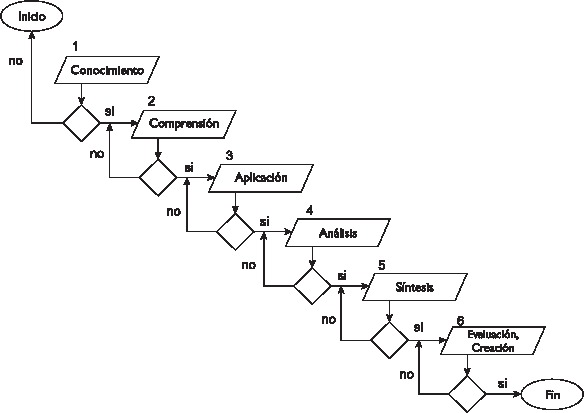
\includegraphics[height=10cm]{../figs/Bloom-sequence}}
		%\Cblur{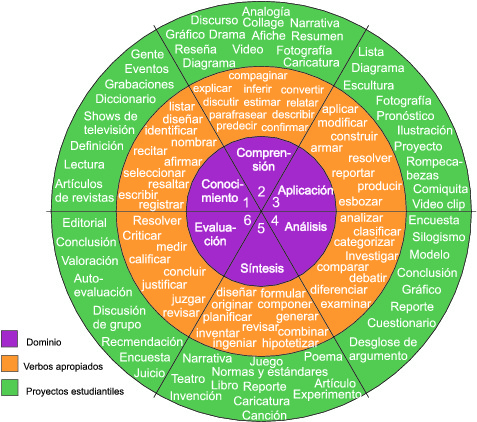
\includegraphics[height=10cm]{../figs/Bloom}}
		%{\captionsize Competencias por disciplina} &
		%{\captionsize Pirámide del Aprendizaje} \\
	\end{tabularx}
}
{	
	~\\
% 	\vspace*{-0.7cm}
	\centering
	\newcommand{\bigstandard}{0.8\textwidth}
	\newcommand{\smallstandard}{0.4\textwidth}
	%\Cblur{\includegraphics[width=\bigstandard]{../figs/curves-\currentarea-with-CS.eps}} \\
	\Cblur{\tcbincludegraphics[hbox,colframe=white,boxrule=0pt,arc=0pt,outer arc=0pt,colback=white,graphics options={width=\bigstandard}]{../figs/curves-\currentarea-with-CS-<LANG_PREFIX>.eps}} \\
	\vspace{0.2cm} 
	\color{white}{\captionsize \bf CS (\siglas) vs CS (ACM/IEEE-CS)}\vspace*{0.2cm}   \\
	\hrule \vspace{0.2cm} 	

	\begin{tabular}{cc}
		\Cblur{\tcbincludegraphics[hbox,colframe=white,boxrule=0pt,arc=0pt,outer arc=0pt,colback=white,graphics options={width=\smallstandard}]{../figs/curves-\currentarea-with-CE-<LANG_PREFIX>.eps}} &
        \Cblur{\tcbincludegraphics[hbox,colframe=white,boxrule=0pt,arc=0pt,outer arc=0pt,colback=white,graphics options={width=\smallstandard}]{../figs/curves-\currentarea-with-IS-<LANG_PREFIX>.eps}} \\
		\color{white}{\captionsize \bf CS (\siglas) vs CE (ACM/IEEE-CS)} & 
		\color{white}{\captionsize \bf CS (\siglas) vs IS (ACM/IEEE-CS)} 
	\end{tabular}
	\hrule \vspace{0.2cm}
	
	\begin{tabular}{cc}
        \Cblur{\tcbincludegraphics[hbox,colframe=white,boxrule=0pt,arc=0pt,outer arc=0pt,colback=white,graphics options={width=\smallstandard}]{../figs/curves-\currentarea-with-SE-<LANG_PREFIX>.eps}} &
        \Cblur{\tcbincludegraphics[hbox,colframe=white,boxrule=0pt,arc=0pt,outer arc=0pt,colback=white,graphics options={width=\smallstandard}]{../figs/curves-\currentarea-with-IT-<LANG_PREFIX>.eps}} \\
		\color{white}{\captionsize \bf CS (\siglas) vs SE (ACM/IEEE-CS)} & 
		\color{white}{\captionsize \bf CS (\siglas) vs IT (ACM/IEEE-CS)} 
 	\end{tabular}
	\hrule \vspace{0.2cm}
	
    \Cblur{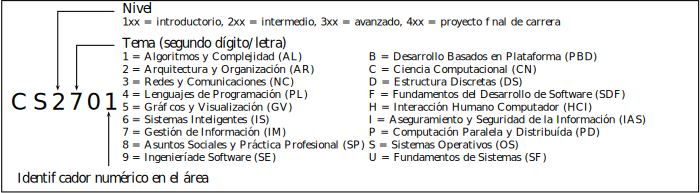
\includegraphics[width=0.965\textwidth]{../figs/course-coding.eps}} \\
	\vspace*{0.1cm}
	\color{white}{\captionsize \bf Codificación de cursos del área de Ciencia de la Computación} \vspace*{0.2cm}\\ \hrule
	\vspace{0.1cm}
% 	\Cblur{\includegraphics[width=0.965\textwidth]{../figs/IS-course-number.eps}} \\
% 		\vspace*{0.2cm}
% 	\color{white}{\captionsize Codificación de cursos del área de Sistemas de Información} \vspace*{0.2cm}\\ \hrule
% 	\hrule
%         \vspace{0.4cm}

	\Cblur{\includegraphics[width=0.965\textwidth]{../figs/\currentarea.eps}} \\
	\vspace*{0.1cm}\color{white}{\captionsize \bf Perfil internacional de CS} \vspace*{0.2cm}\\ \hrule
	\hrule \vspace{0.4cm}

	\begin{tabularx}{0.95\textwidth}{m{.5cm}cm{.5cm}Xm{.5cm}}
		% 		\Cblur{\includegraphics[heigth=6.55cm]{../figs/pie-credits.eps}} &
		% 		\Cblur{\includegraphics[heigth=6.55cm]{../figs/pie-by-levels.eps}} \\
		%		\Cblur{\includegraphics[height=6.55cm]{../figs/pie-credits.eps}} & & \Cblur{\includegraphics[height=6.55cm]{../figs/pie-by-levels.eps}} \\
		%		\color{white}{\captionsize \bf Créditos por área} 				& & \color{white}{\captionsize \bf Créditos por nivel}
		&
		\begin{minipage}{0.4\textwidth}
			\centering
			\Cblur{\tcbincludegraphics[hbox,colframe=white,boxrule=0pt,arc=0pt,outer arc=0pt,colback=white,graphics options={height=6.1cm}]{../figs/pie-credits.eps}}
			\color{white}{\captionsize \bf Créditos por área}
		\end{minipage}
		& &
		\begin{minipage}{0.6\textwidth}
			\centering 
			% colback=olive
			\Cblur{\tcbincludegraphics[hbox,colframe=white,boxrule=0pt,arc=0pt,outer arc=0pt,colback=white,graphics options={height=6.1cm}]{../figs/pie-by-levels.eps}} \\
			\color{white}{\captionsize \bf Créditos por nivel}
		\end{minipage}
		&
	\end{tabularx}
}

\Cblur{ 
	\begin{tabularx}{\textwidth}{X}%
	\textbf{Definición de Objetivos de Aprendizaje ({\it Learning Outcomes})} 				\\ \hline
		%\vspace{0.01cm}
		{\textbf{Nivel 1 \Familiarity\xspace({\it Familiarity})}: \LearningOutcomesTxtEsFamiliarity} 	\\
		{\textbf{Nivel 2 \Usage\xspace({\it Usage})}: \LearningOutcomesTxtEsUsage} 						\\
		{\textbf{Nivel 3 \Assessment\xspace({\it Assessment})}: \LearningOutcomesTxtEsAssessment} \\ %
	\end{tabularx}%
}

\Cblur{\begin{minipage}{\textwidth}\textbf{\large \Copyrights}\end{minipage}}

\end{document}
